% Chapter Template

\chapter{Datos} % Main chapter title

\label{Cap_Data} % Change X to a consecutive number; for referencing this chapter elsewhere, use \ref{ChapterX}


%Justificación de la importancia de graficar los datos antes de realizar análisis estadísticos.
Previo a la realización de los análisis estadísticos correspondientes para responder la interrogante planteada respecto de la existencia de los patrones identificados como parte del Efecto Espejo en Memoria de Reconocimiento, en una tarea de detección perceptual, los datos obtenidos fueron explorados de manera exhaustiva graficando las posibles correlaciones entre la ejecución de los participantes y diversas variables operantes en el mismo. Graficar los datos antes de someterlos a un análisis constituye una práctica altamente recomendable, ya que 1) permite evaluar la pertinencia de los experimentos propuestos a la luz de las respuestas obtenidas por los participantes y 2) constituye un primer filtro para descartar la posibilidad de que los participantes estuvieren respondiendo de manera incongruente con las tareas presentadas, procurando tener una mayor confianza en las conclusiones que puedan extraerse de su análisis.\\

%Presentación de los controles graficados: Atención, El efecto del paso del tiempo y las variables externas en los estímulos. 
En este capítulo se presentan gráficas que exploran la posible relación que pudieran tener las respuestas de los participantes con cualquier variable ajena a las demandas de la tarea, como podrían ser las respuestas inmediatamente anteriores (i.e. trenes de respuesta), el paso del tiempo (i.e. aprendizaje) y las propiedades de los estímulos diseñados (i.e. sesgo). Idealmente, se esperaría que el desempeño de los participantes no mostrara cambios a lo largo del tiempo y no variara en función a ninguna característica de los estímulos construidos que no sea el número de círculos externos en las figuras de Ebbinghaus, (i.e. la variable independiente).\\


\section{Control 1: ¿Los participantes estaban poniendo atención a la tarea para emitir una respuesta?}

%Evaluando la atención: Que
Los experimentos realizados estuvieron compuestos de 640 ensayos a lo largo de los cuales los participantes tuvieron que 1) decidir si los estímulos presentados cumplían con la condición que se les solicitó detectar y 2) valorar su certidumbre sobre esta primer respuesta asignándole un puntaje. Dada la extensión y lo demandante del procedimiento, la primer preocupación era que los participantes se agotaran y dejaran de poner atención a la tarea al emitir sus respuestas. Para controlar esta posibilidad, se revisaron las respuestas emitidas ensayo a ensayo para verificar que todas las opciones de respuesta fueran utilizadas para cada tarea planteada y que no se presentaran trenes de respuesta que pudieran sugerir una emisión de respuestas independiente del contenido de la tarea.\\

\begin{itemize}
\item Emisión de respuestas 'Sí/No' a lo largo del experimento.

Primero se graficaron las respuestas emitidas ensayo a ensayo durante la tarea de detección binaria ('Sí, los círculos son iguales', 'No, los círculos son diferentes'). El objetivo principal de estas gráficas fue el de detectar trenes de respuesta prolongados que, dada la aleatoriedad con que los estímulos fueron presentados por el programa, pudieran delatar un sesgo del participante a presionar una tecla en particular independientemente del estímulo a evaluar en pantalla.\\

%Participante representativo: Respuestas 'No' por 80 ensayos
La Figura~\ref{fig:Resp_E1_P1} ilustra la importancia de revisar los datos antes de incluirlos en el análisis estadístico y extraer conclusiones, al presentar las respuestas emitidas a la tarea de detección binaria por el Participante 1 del Experimento 1, quien pasó los primeros 80 ensayos del experimento respondiendo repetidamente a la tecla 'No'. Este tren de respuesta es lo suficientemente largo como para cuestionar la atención con que el Participante 1 estuvo respondiendo a la tarea.\\ 

\begin{figure}[th]
\centering
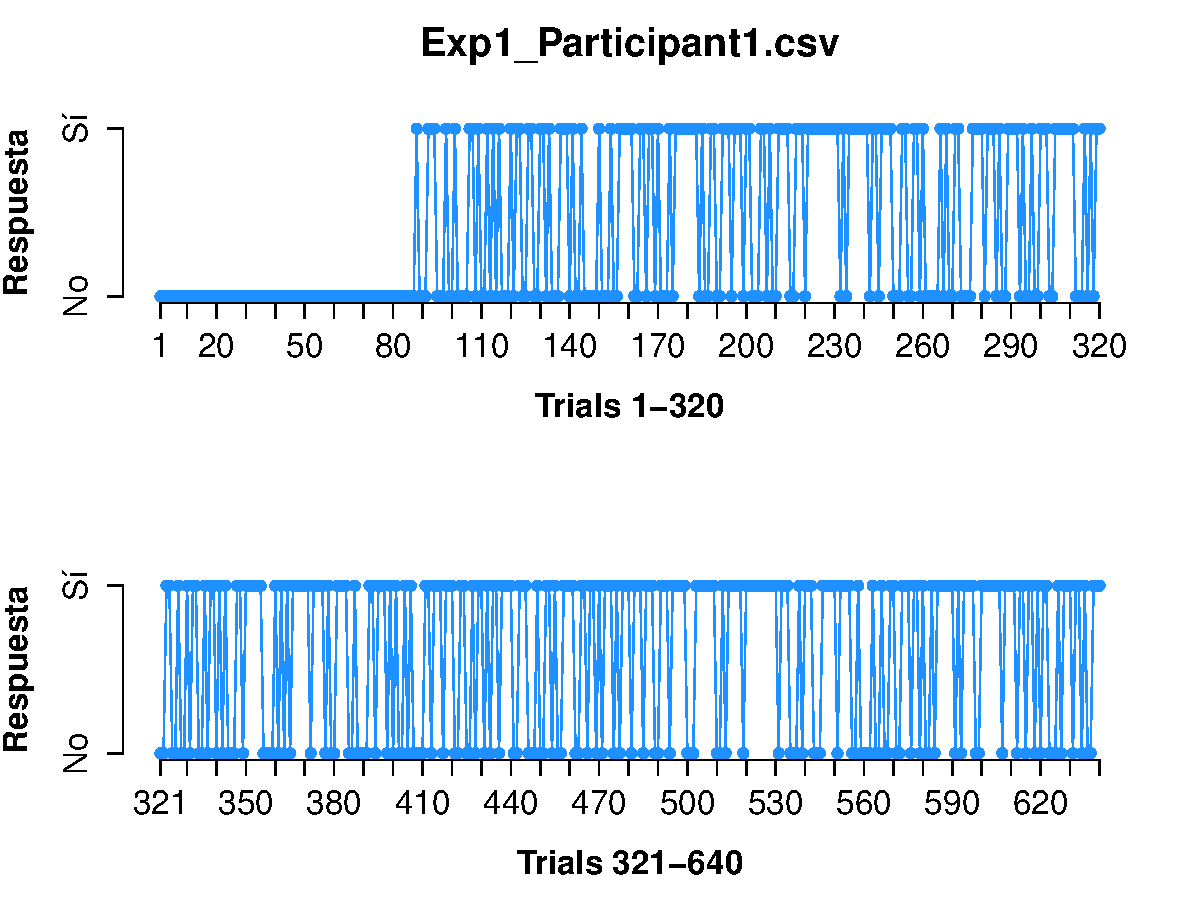
\includegraphics[width=0.60\textwidth]{Figures/Response_Exp1_P1} 
%\decoRule
\caption[Respuesta emitida por ensayo; ejemplo de participante sesgado]{Se muestran las respuestas ('Sí/No') emitidas en cada uno de los 640 ensayos del Experimento 1 por el Participante 1. La gráfica superior muestra los primeros 320 ensayos y la gráfica inferior, los 320 restantes. En el panel superior se aprecia con claridad un tren de respuesta que se extiende a lo largo de 80 ensayos, durante los cuales el Participante 1 sólo utilizó una de las opciones de respuesta.}
\label{fig:Resp_E1_P1}
\end{figure}

Las gráficas correspondientes al resto de los participantes en los Experimentos 1 y 2, se muestran en las Figuras~\ref{fig:Response_P1} y \ref{fig:Response_E2}, respectivamente.\\

\item Correlación entre las respuestas 'Sí/No' emitidas y el tipo de estímulo presentado en cada ensayo.

A continuación, se graficaron las respuestas emitidas por los participantes en cada ensayo añadiendo indicadores que señalaran las características de los estímulos presentados; en concreto, si se trataba de una señal o ruido y si se trataba de un estímulo fácil o difícil.\\ 

Retomando el caso del Participante 1 del Experimento 1 presentado en la Figura~\ref{fig:Resp_E1_P1}, la Figura~\ref{fig:BiasResp_E1_P1} explora la posible correlación entre las respuestas registradas y el tipo de estímulo presentado en cada ensayo. Sin embargo, parece ser que el tren de 80 respuestas 'No' consecutivas se mantiene con independencia del tipo de estímulo presentado. Con base en dicha evidencia, se decidió eliminar al Participante 1 del Experimento 1 del análisis estadístico, pues se cree que se tiene razones suficientes para dudar de la atención que el participante estaba prestando al responder a la tarea.\\

\begin{figure}[th]
\centering
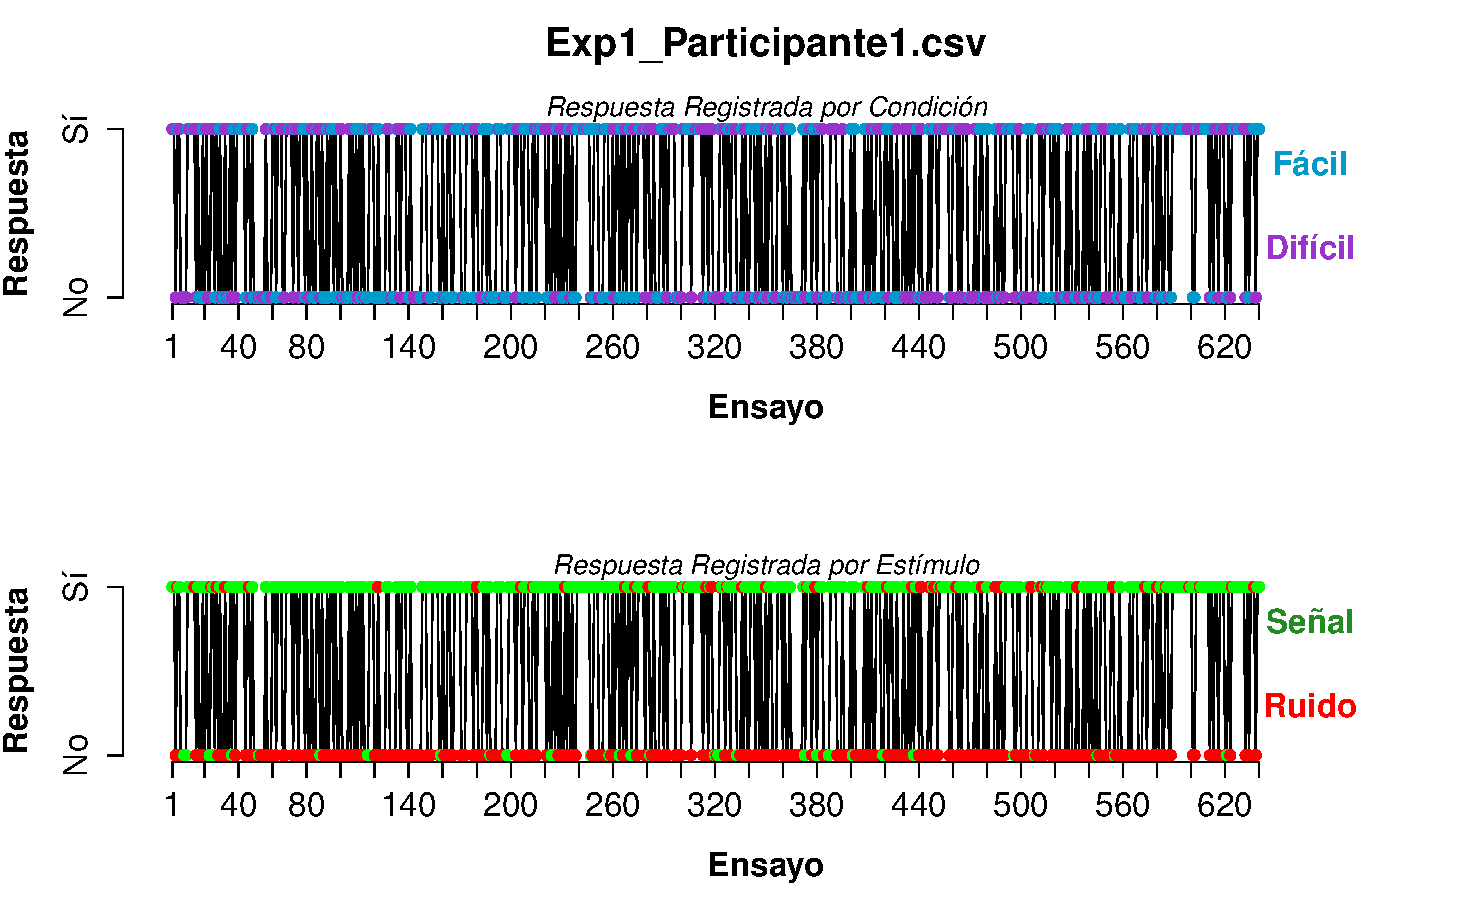
\includegraphics[width=0.60\textwidth]{Figures/BiasResp_Exp1_P1} 
%\decoRule
\caption[Respuesta por Tipo de Estimulo; ejemplo de participante sesgado]{Se muestran las respuestas registradas por el Participante 1 en cada uno de los ensayos del Experimento 1, indicando con diferentes colores el tipo de estímulo que se le mostraba en cada ocasión. En el panel superior se señala con colores violeta y azul si el estímulo presentado pertenecía a la categoría Difícil o Fácil, respectivamente. En el panel inferior se indica si se trataba de una señal o ruido, señalándolos con los colores verde y rojo, respectivamente.}
\label{fig:BiasResp_E1_P1}
\end{figure}

Las Figuras~\ref{fig:BiasResp_E1} y () muestran las gráficas correspondientes al resto de los participantes en el Experimento 1 y 2, respectivamente.\\

\item Asignación de puntajes de confianza, ('1','2' y '3').

En la segunda fase de la tarea, los participantes tenían tres opciones de respuesta (teclas '1', '2' y '3') para señalar qué tanta confianza tenían sobre la respuesta previa ('poco seguro', 'más o menos seguro' o 'muy seguro', respectivamente). Las respuestas emitidas eran registradas por el programa de acuerdo a una escala mayor, (con valores del 1 al 6), que diferencía entre la confianza de haber rechazado correctamente un estímulo con ruido (e.g. '1, estoy seguro de que los círculos eran diferentes') y la confianza de haber identificado correctamente un estímulo con la señal a detectar (e.g '6, estoy seguro de que los círculos son iguales'), dejando los valores intermedios de la escala (3 y 4) para los puntajes que correlacionaran con una confianza baja en la respuesta emitida (e.g. '3, poco seguro de que los círculos eran diferentes' y '4, poco seguro de que los círculos eran iguales').\\

Tal y como se hizo para la tarea de detección binaria, se graficaron los puntajes de confianza asignados por los participantes en cada uno de los 640 ensayos que conformaron los experimentos. La Figura~\ref{fig:Rating_E2_P4} muestra los puntajes emitidos por el Participante 15 del Experimento 1 a lo largo de la tarea. Este participante, de acuerdo con lo que se esperaría de alguien que estuviere prestando atención a la tarea, utiliza todas las opciones de respuesta (teclas '1', '2' y '3'), siendo estas registradas por el programa de acuerdo con la respuesta dada a la tarea de detección binaria ('1' como '3' o '4', '2' como '2' o '5', '3' como '1' o '6'; dependiendo si la respuesta previa fue un 'no' o un 'sí', respectivamente). 
 
\begin{figure}[th]
\centering
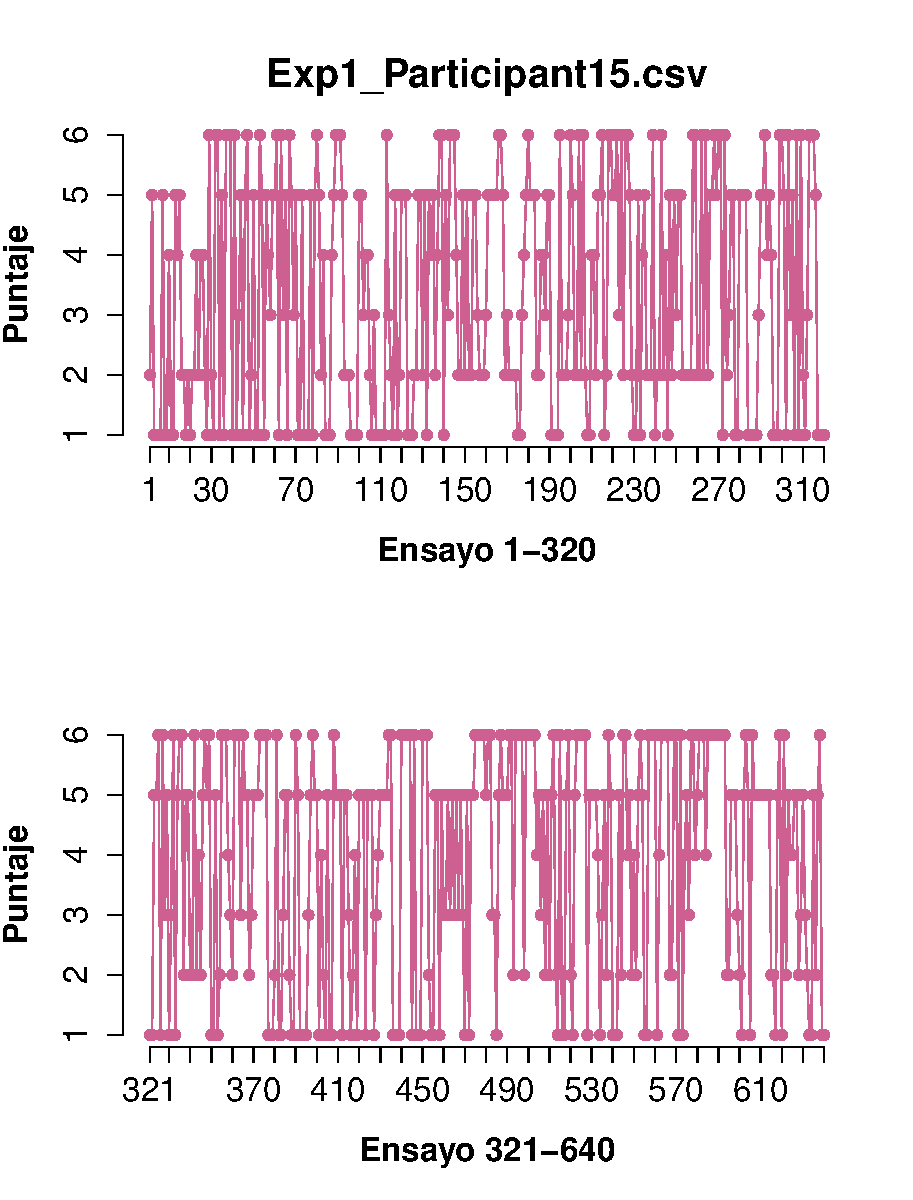
\includegraphics[width=0.50\textwidth]{Figures/Rating_Exp1_P15} 
%\decoRule
\caption[Asignacion Puntaje de confianza: Participante con multiples elecciones]{Se muestran los puntajes de confianza asignados por el Participante 15 del Experimento 1 a las respuestas emitidas en la tarea binaria, durante cada uno de los 640 ensayos que conforman el experimento. El panel superior muestra los puntajes asignados en los primeros 320 ensayos del experimento; el panel inferior, muestra los 320 restantes.}
\label{fig:Rating_E2_P4}
\end{figure}

El registro ensayo a ensayo de los puntajes de confianza asignados por el resto de los participantes en los Experimentos 1 y 2 se muestran en las Figuras~\ref{fig:Rating_E1} y \ref{fig:Rating_E2}, respectivamente.

\end{itemize}



\begin{figure}[th]
\centering
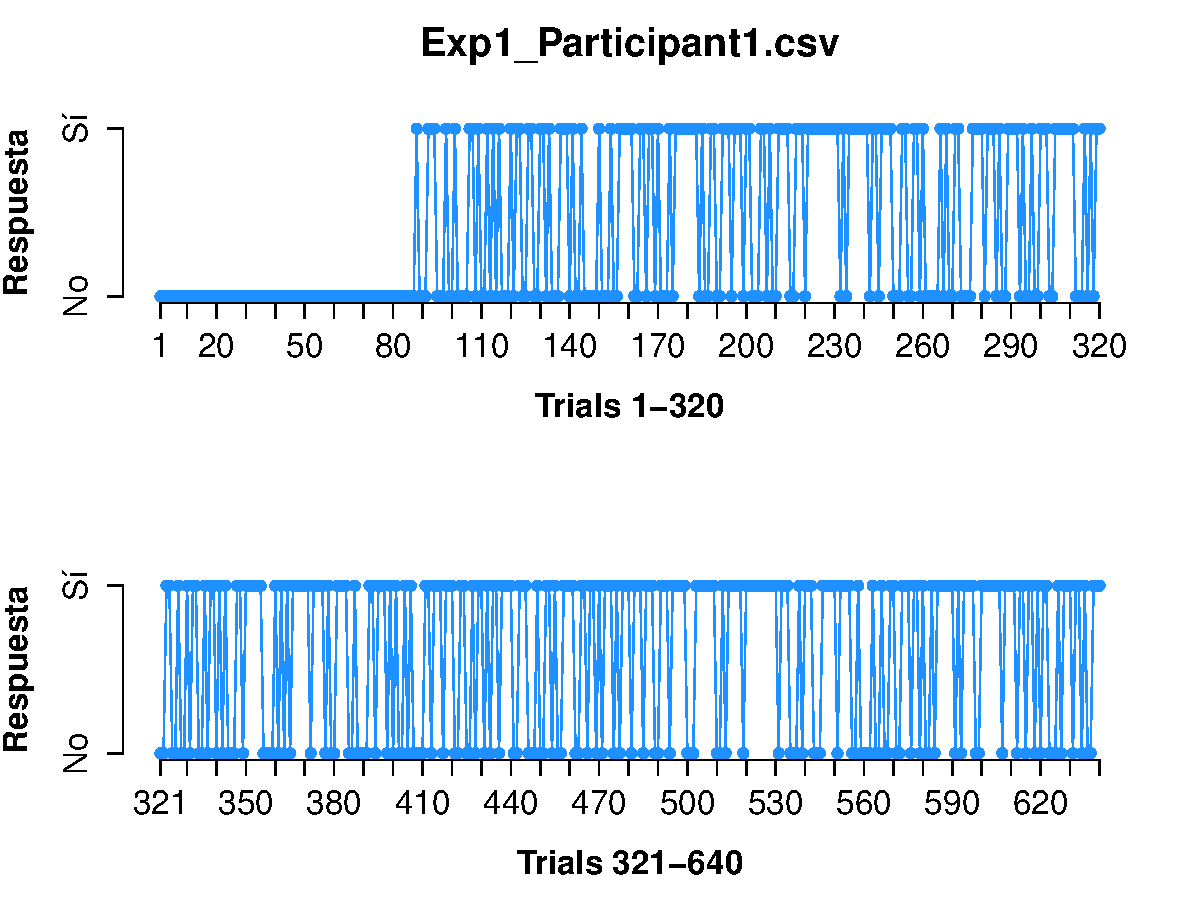
\includegraphics[width=0.30\textwidth]{Figures/Response_Exp1_P1} 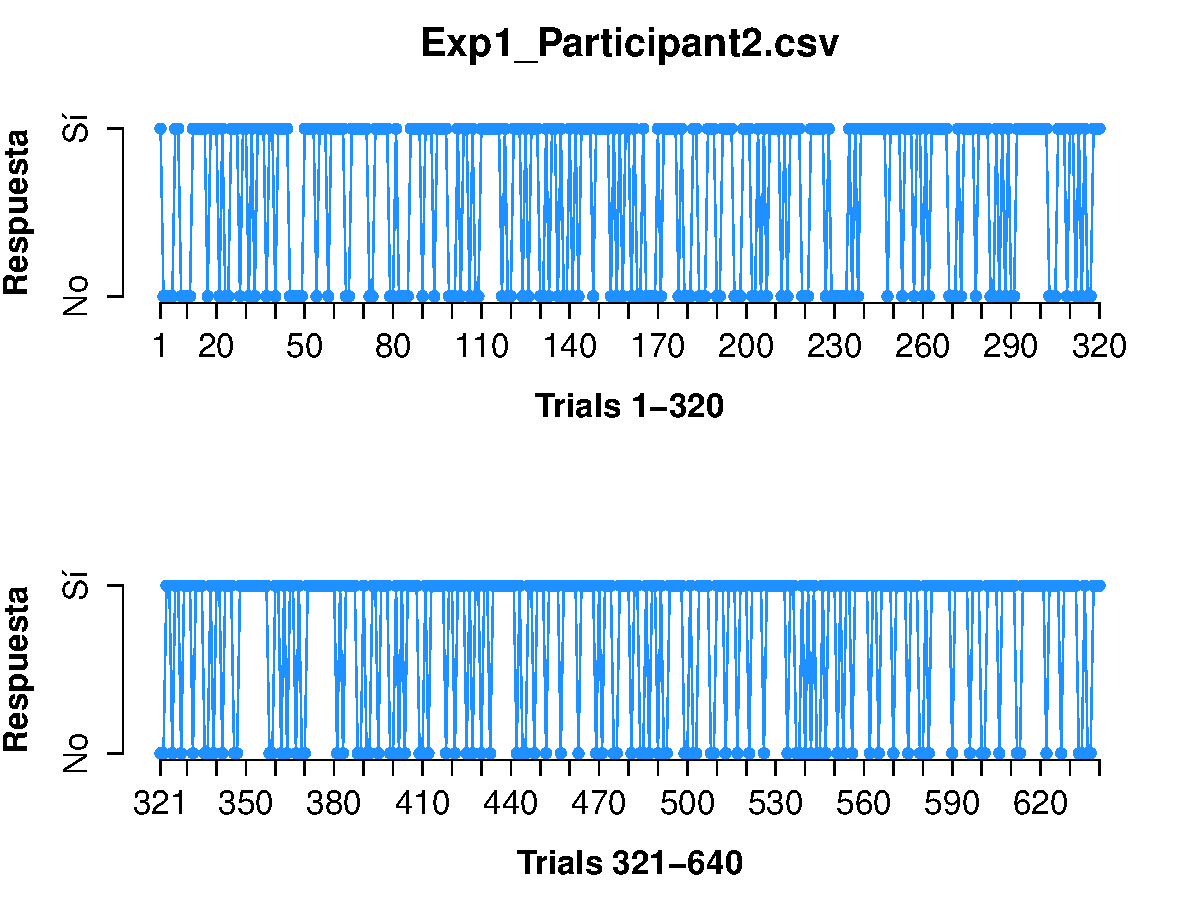
\includegraphics[width=0.30\textwidth]{Figures/Response_Exp1_P2} 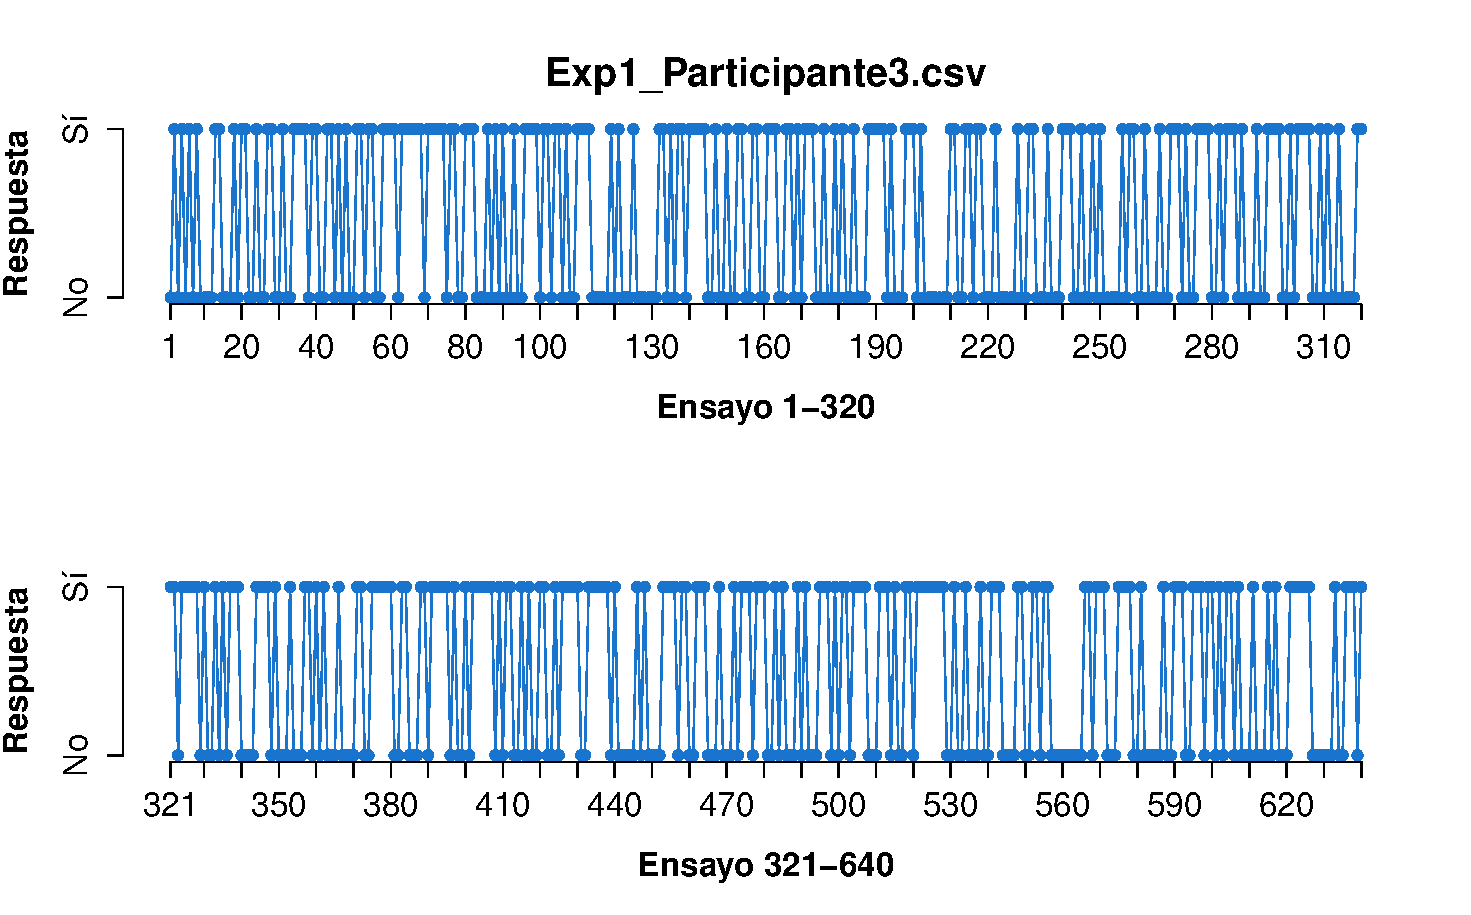
\includegraphics[width=0.30\textwidth]{Figures/Response_Exp1_P3}
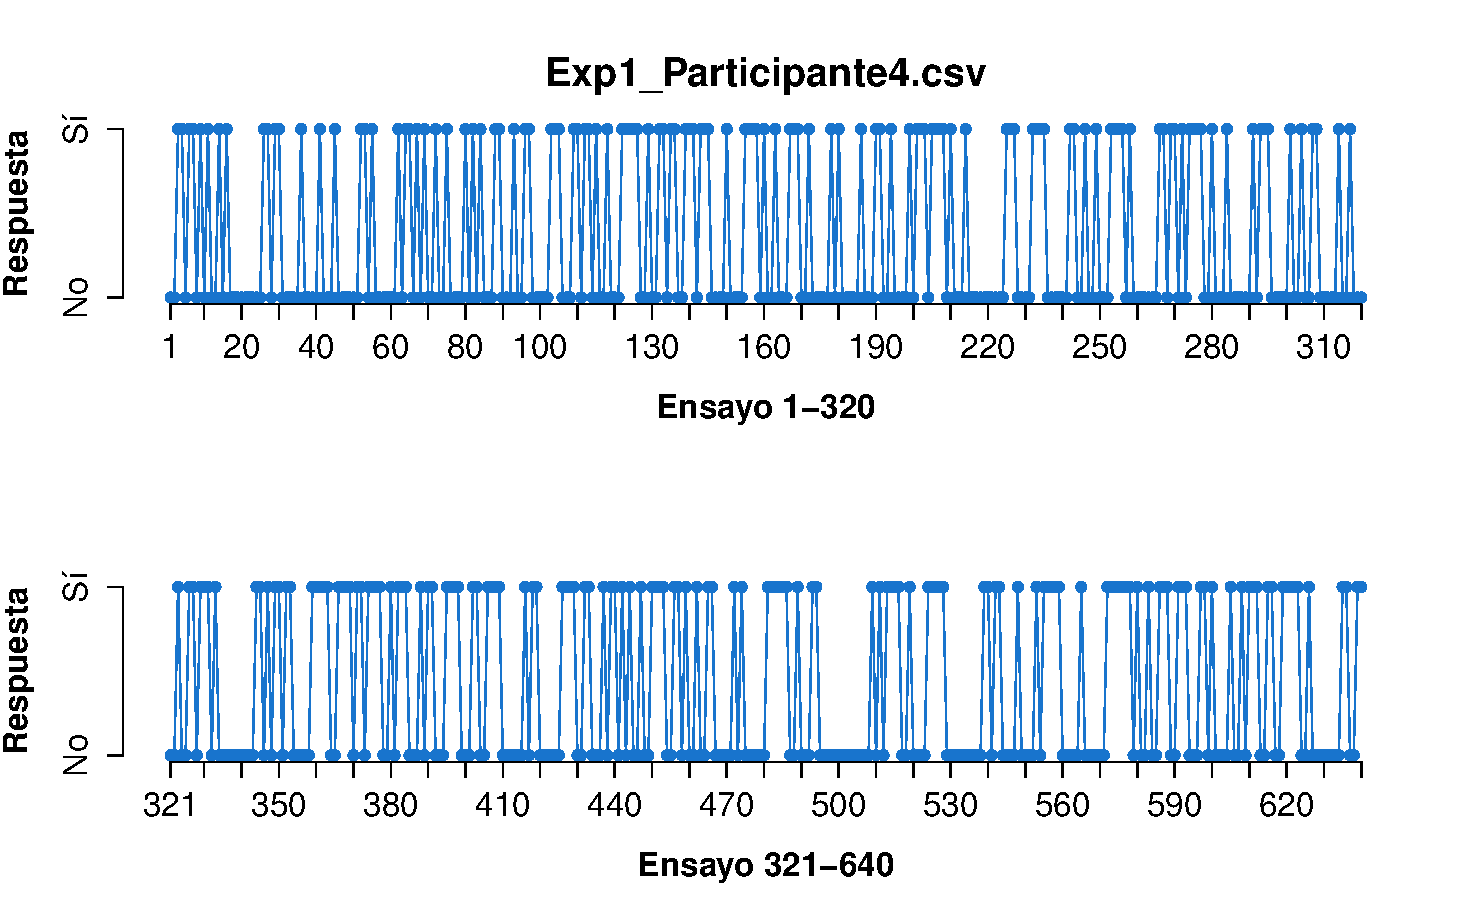
\includegraphics[width=0.30\textwidth]{Figures/Response_Exp1_P4} 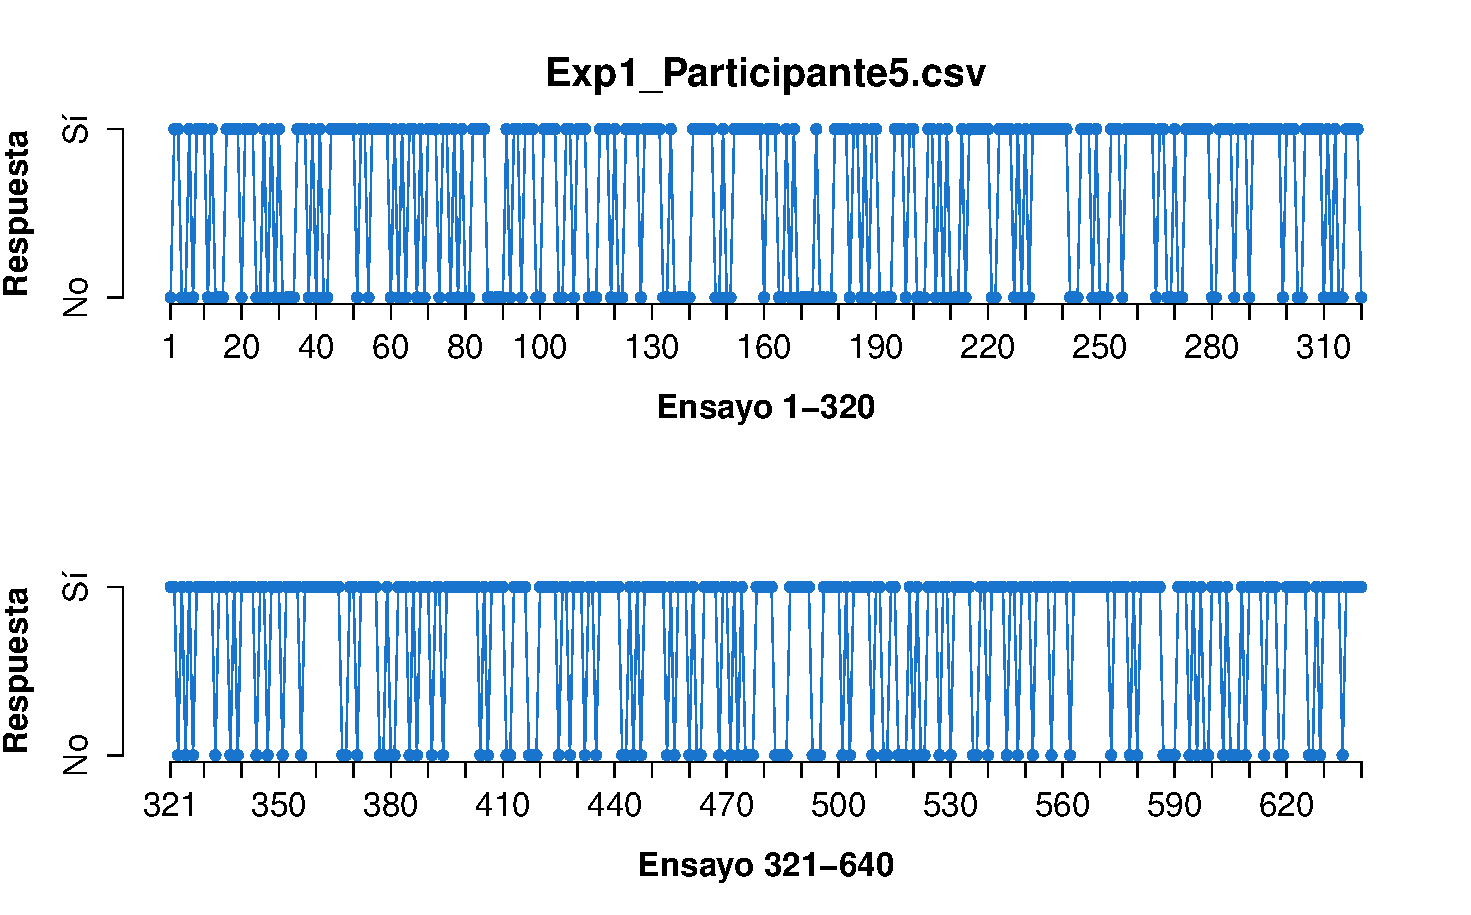
\includegraphics[width=0.30\textwidth]{Figures/Response_Exp1_P5} 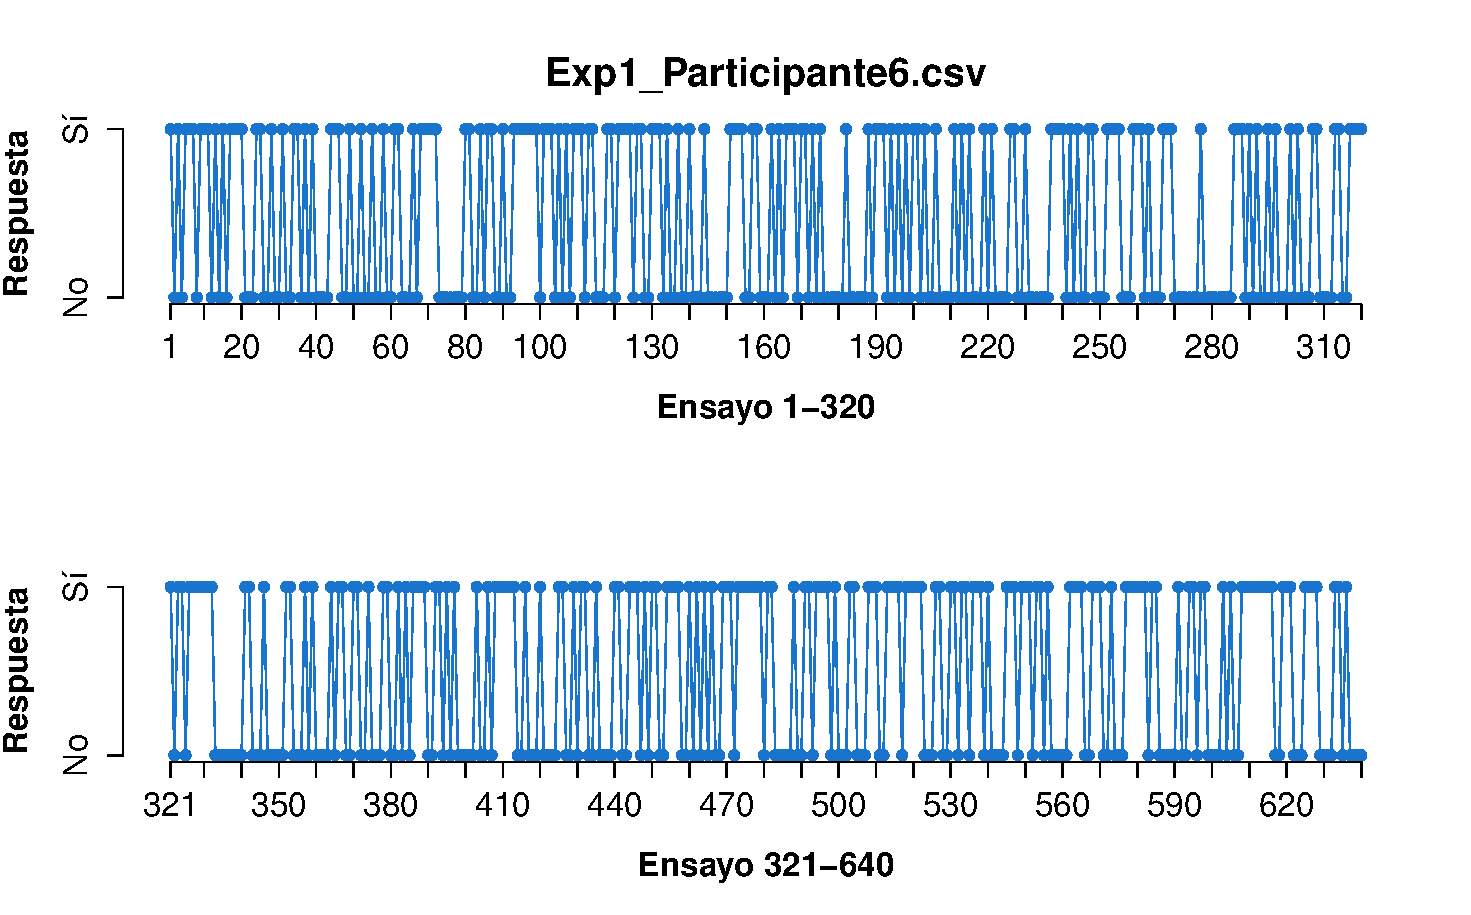
\includegraphics[width=0.30\textwidth]{Figures/Response_Exp1_P6}
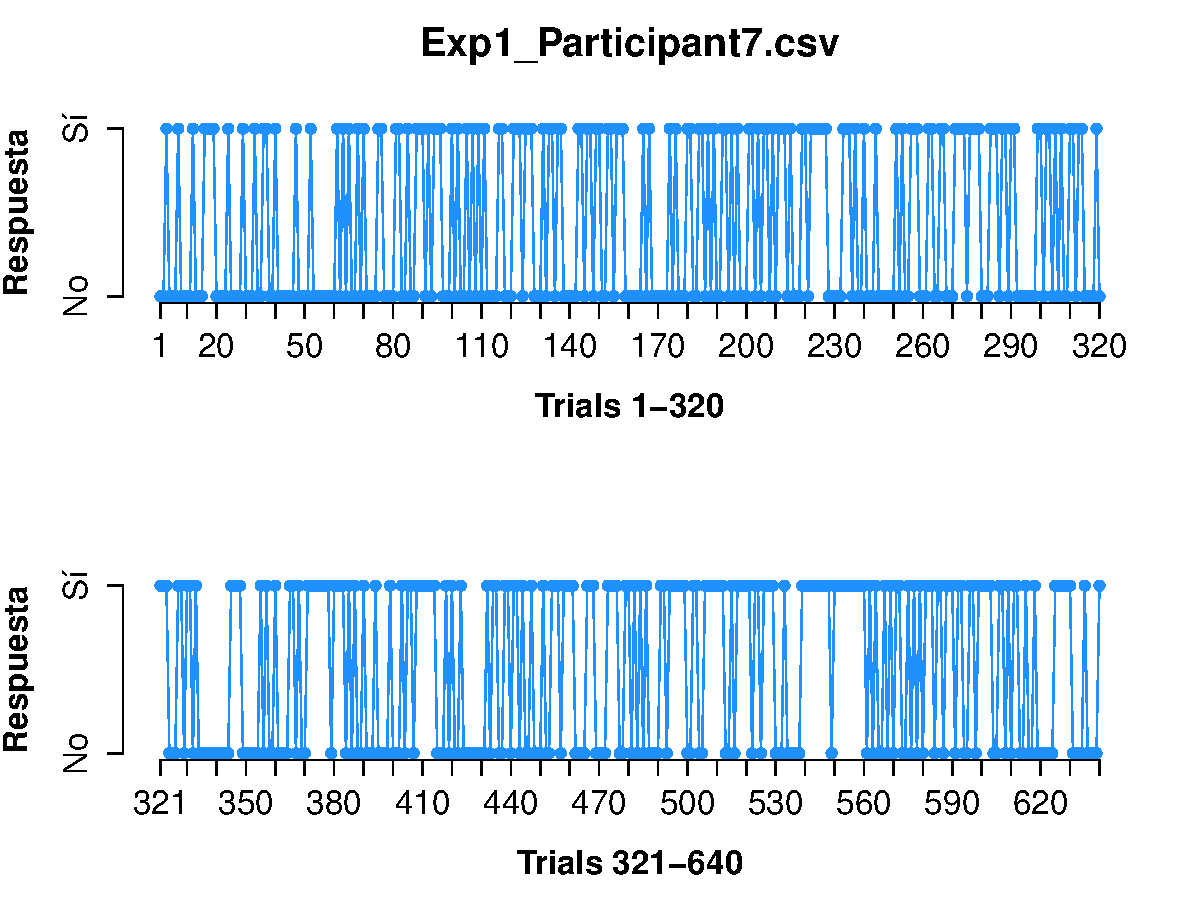
\includegraphics[width=0.30\textwidth]{Figures/Response_Exp1_P7} 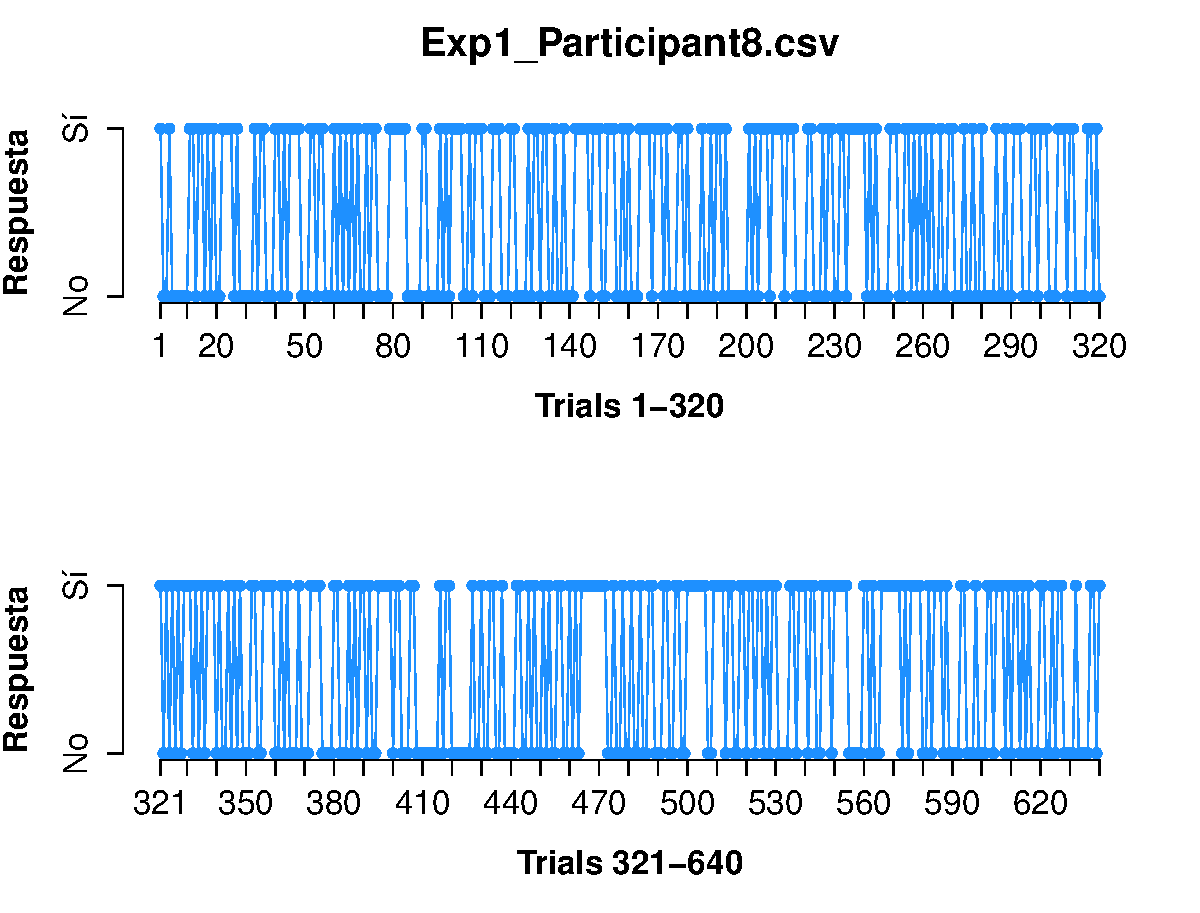
\includegraphics[width=0.30\textwidth]{Figures/Response_Exp1_P8} 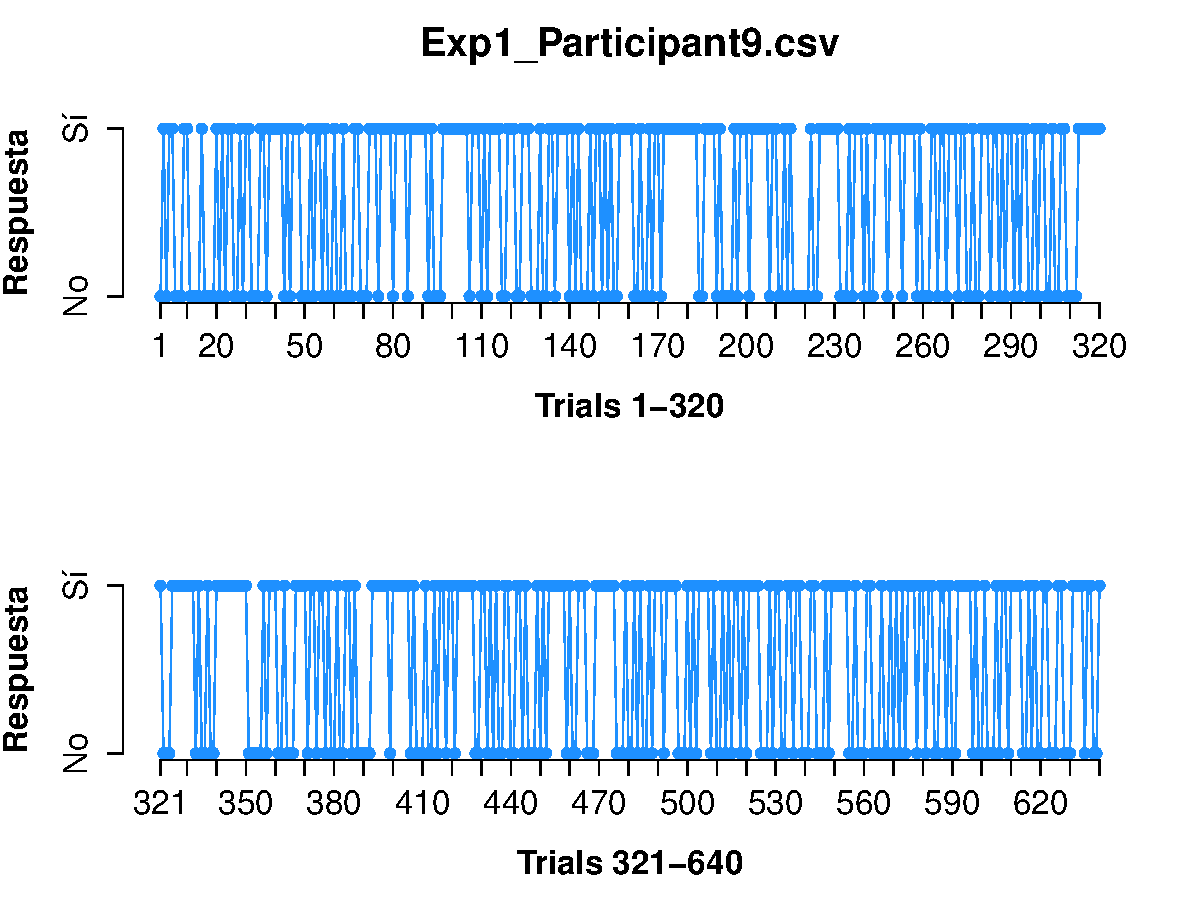
\includegraphics[width=0.30\textwidth]{Figures/Response_Exp1_P9}
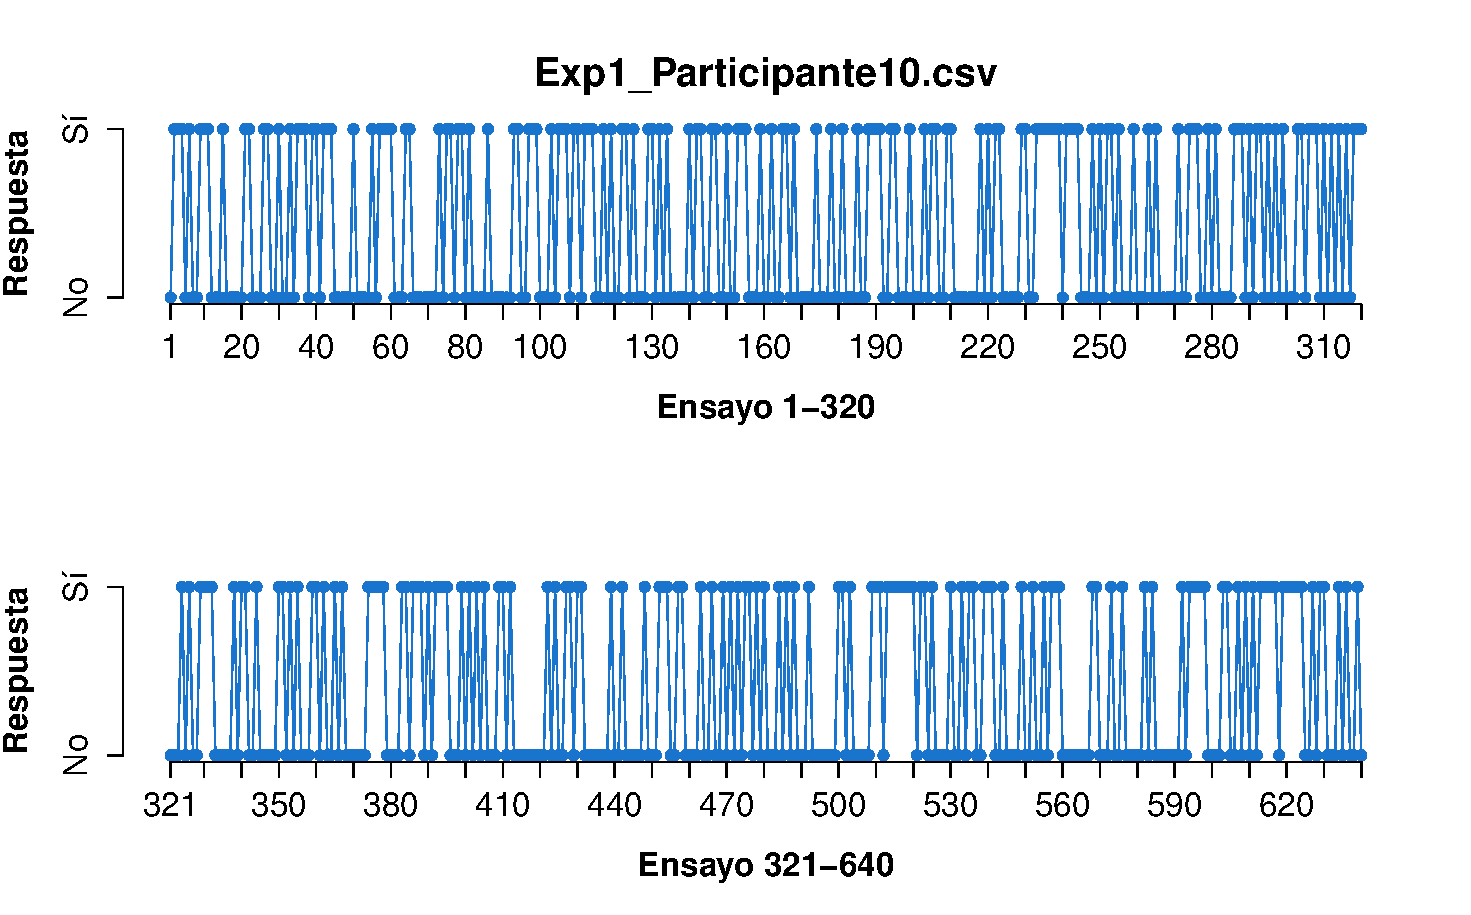
\includegraphics[width=0.30\textwidth]{Figures/Response_Exp1_P10} 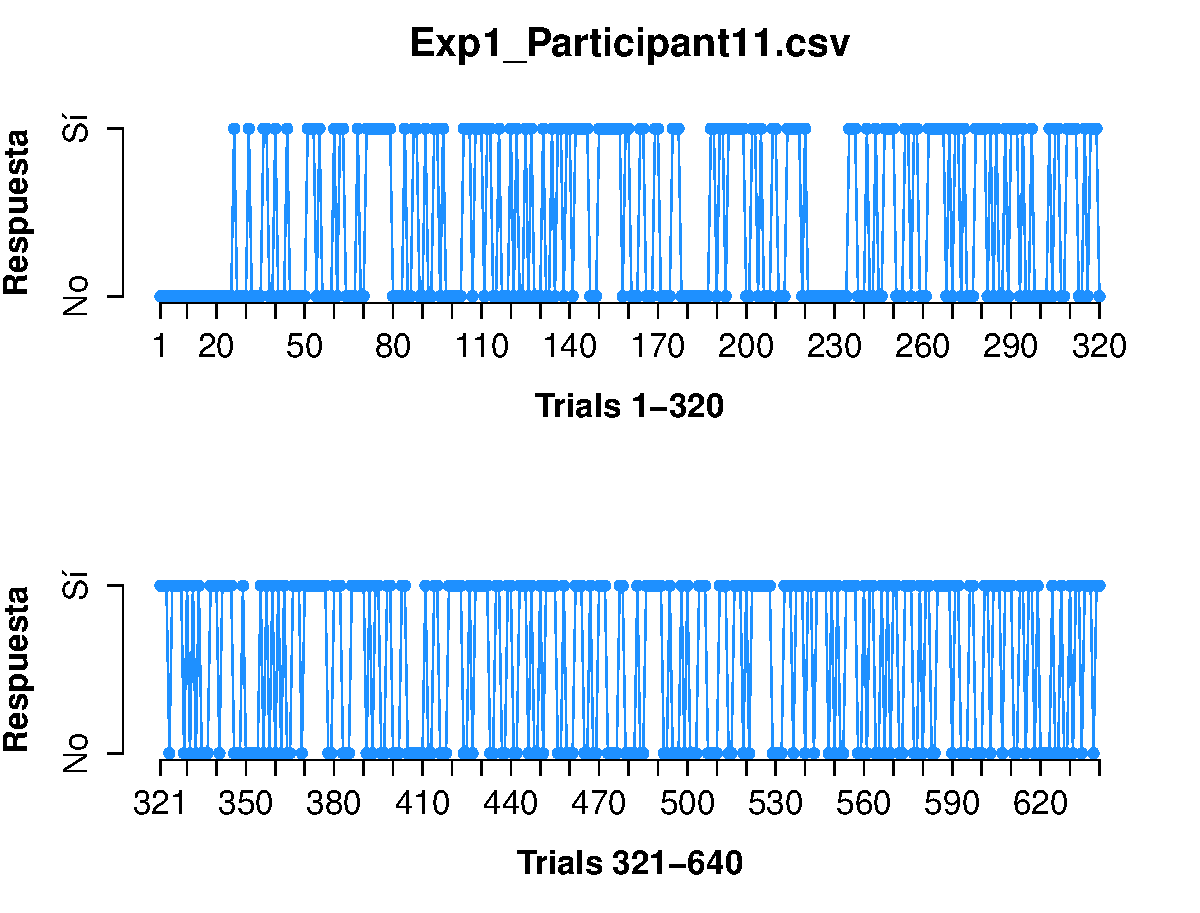
\includegraphics[width=0.30\textwidth]{Figures/Response_Exp1_P11} 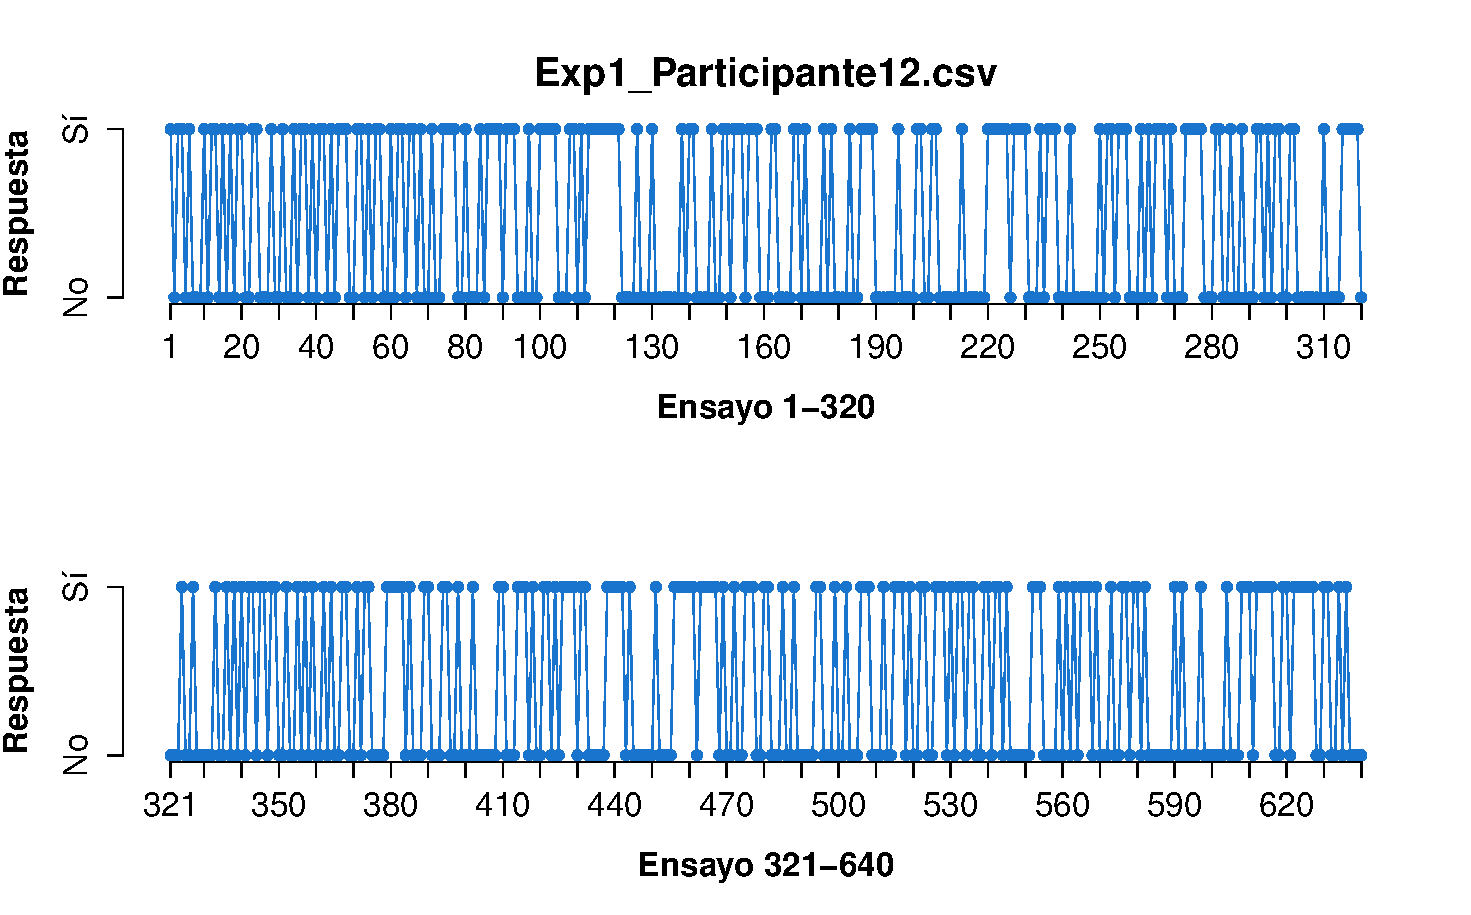
\includegraphics[width=0.30\textwidth]{Figures/Response_Exp1_P12}
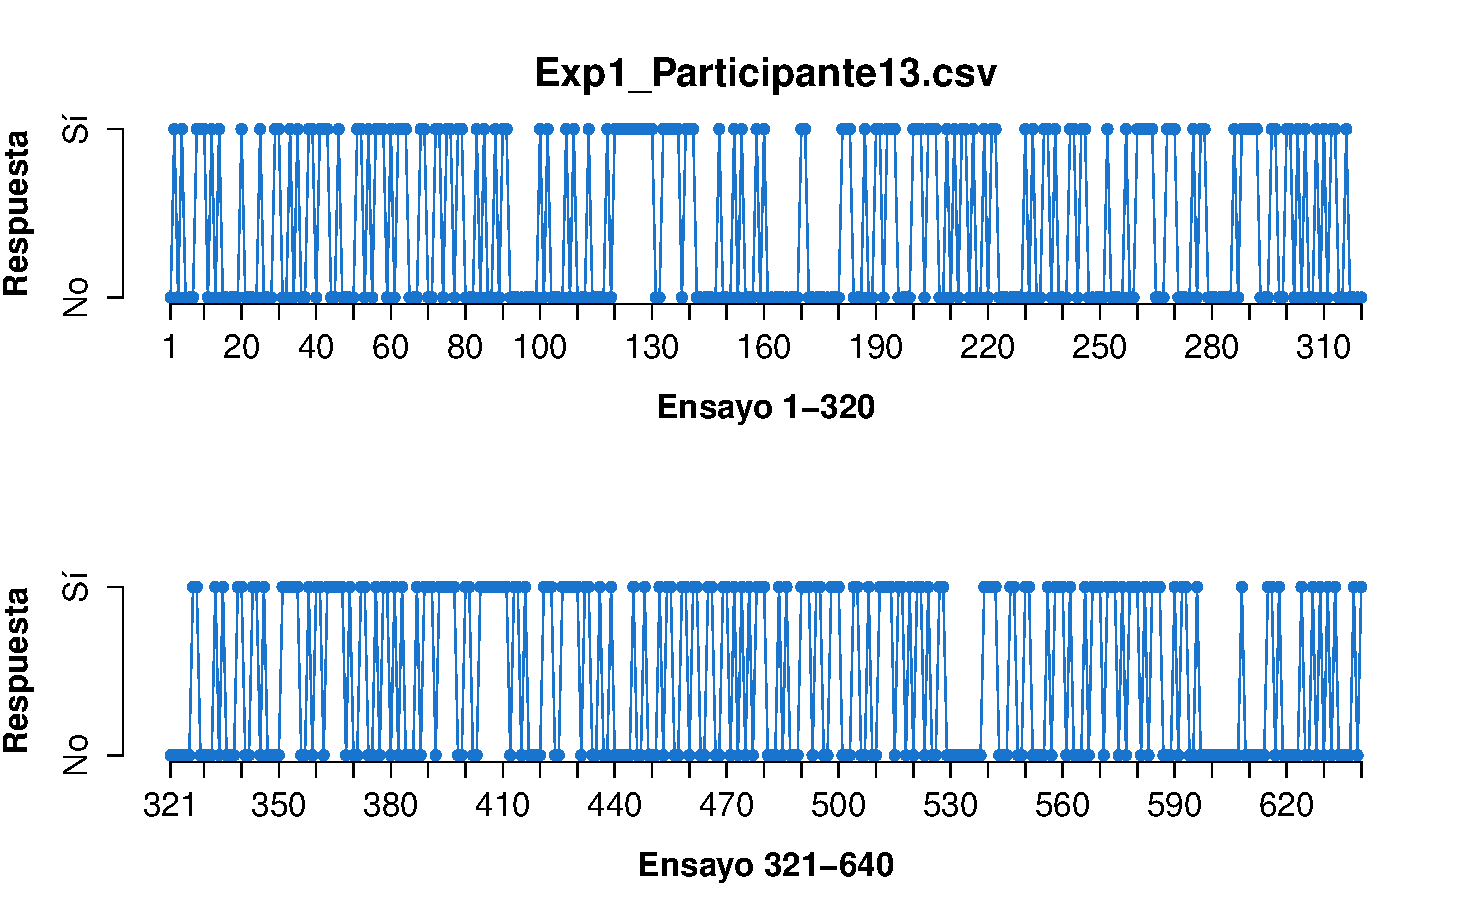
\includegraphics[width=0.30\textwidth]{Figures/Response_Exp1_P13} 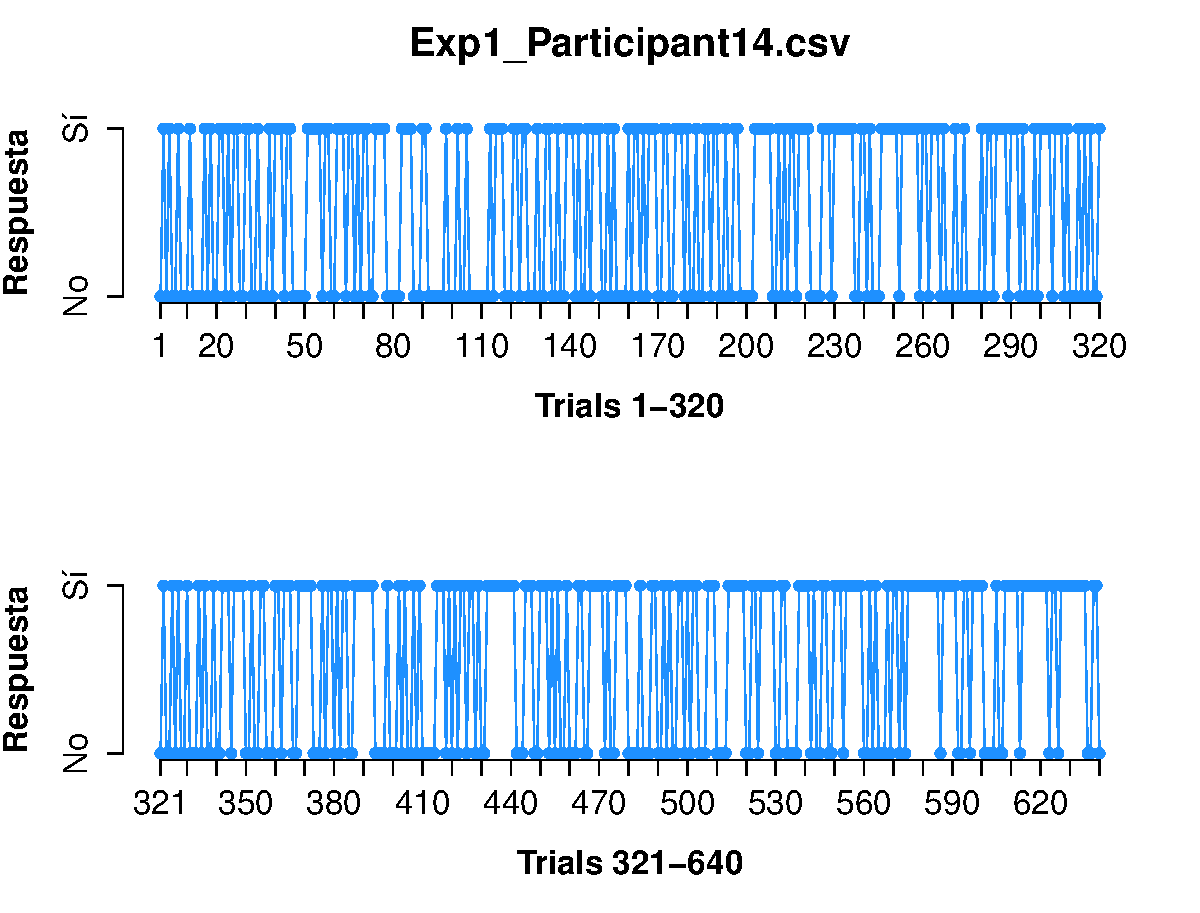
\includegraphics[width=0.30\textwidth]{Figures/Response_Exp1_P14} 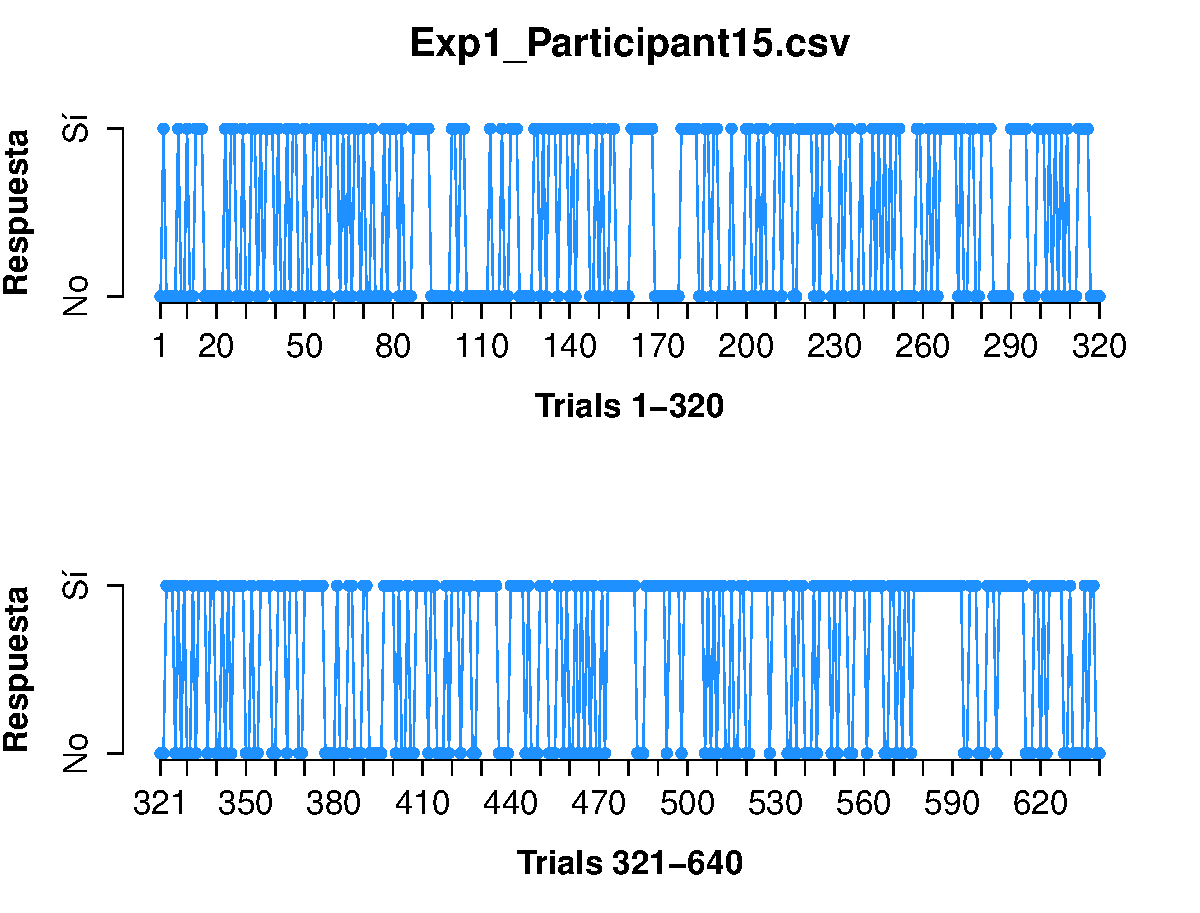
\includegraphics[width=0.30\textwidth]{Figures/Response_Exp1_P15}
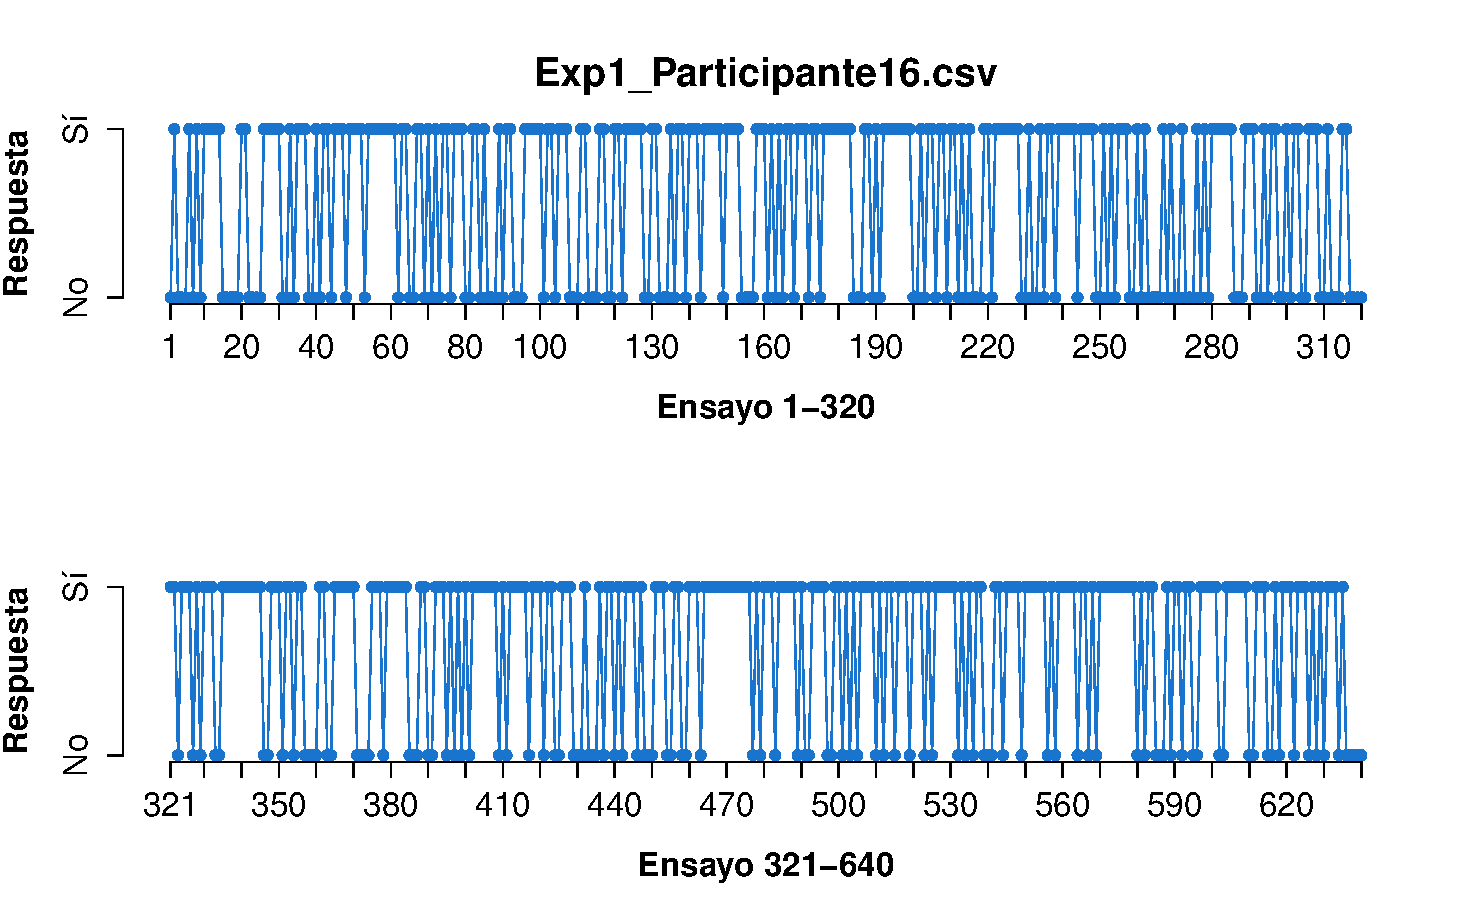
\includegraphics[width=0.30\textwidth]{Figures/Response_Exp1_P16} 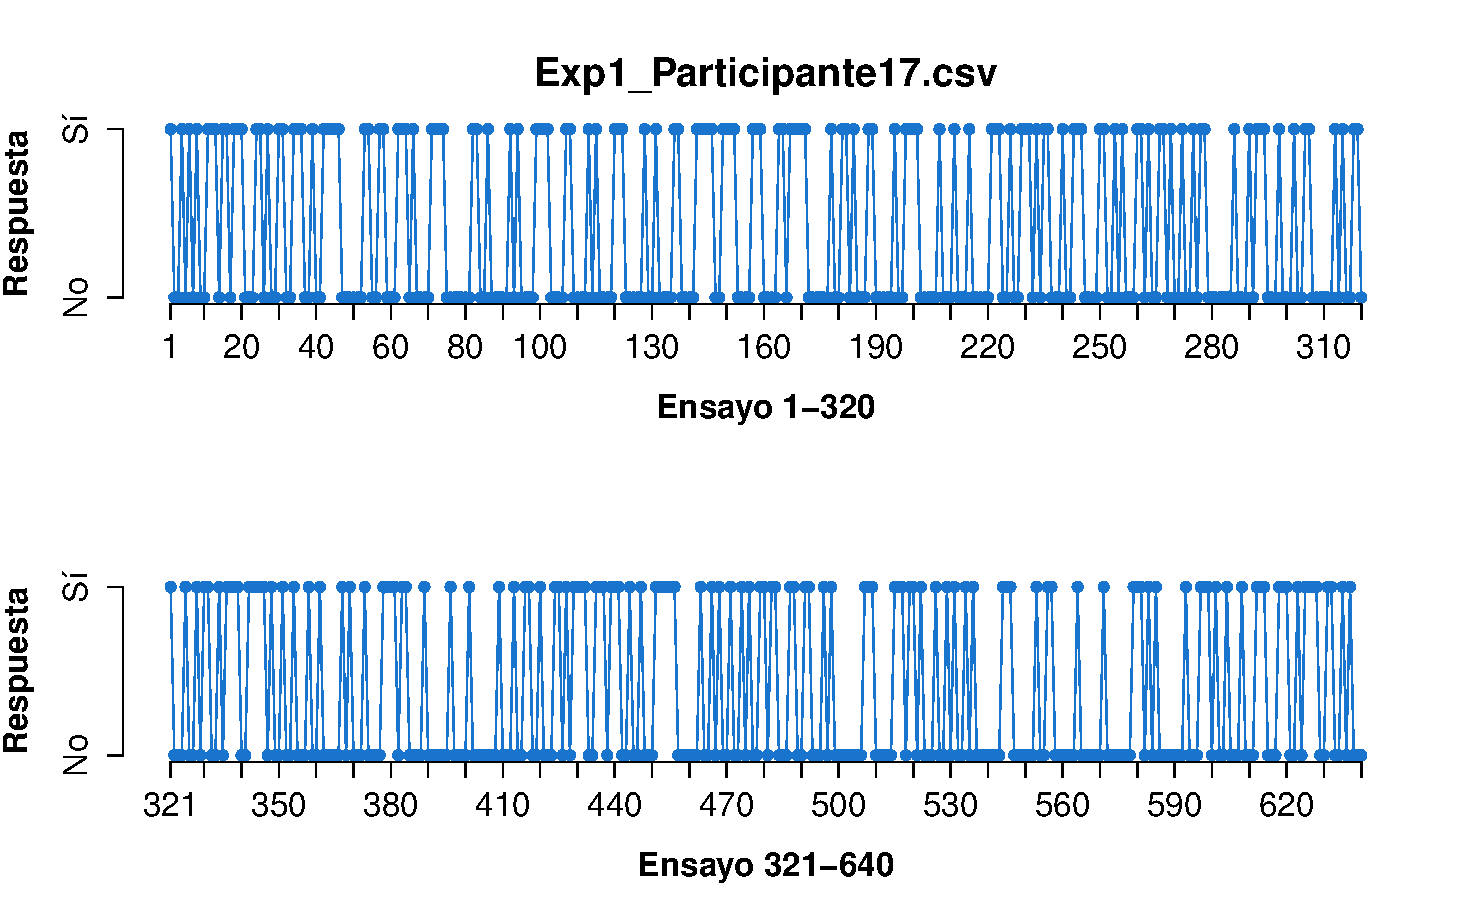
\includegraphics[width=0.30\textwidth]{Figures/Response_Exp1_P17} 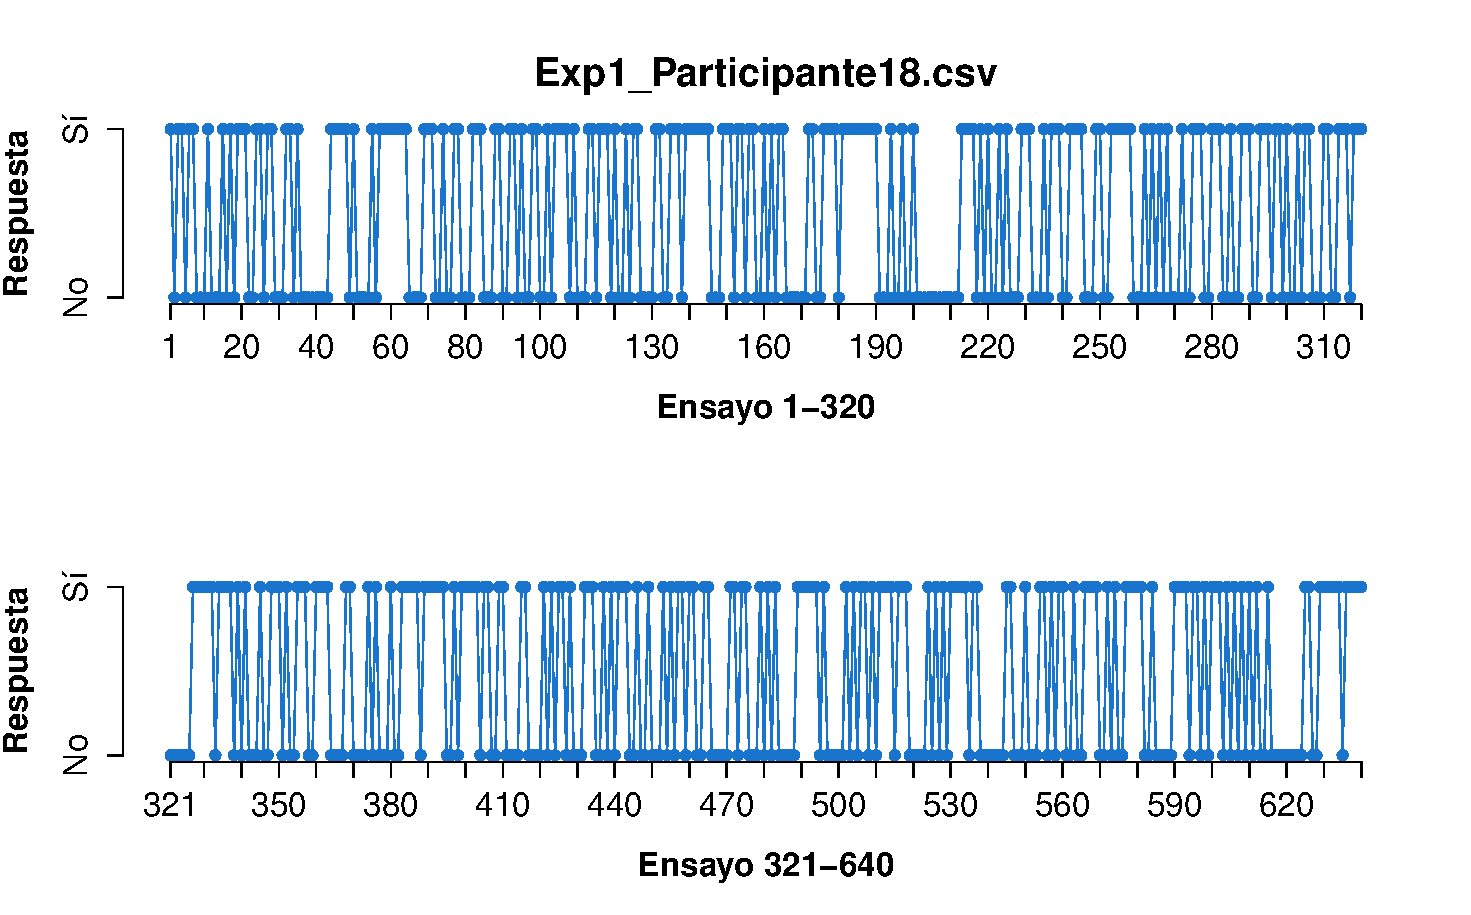
\includegraphics[width=0.30\textwidth]{Figures/Response_Exp1_P18}
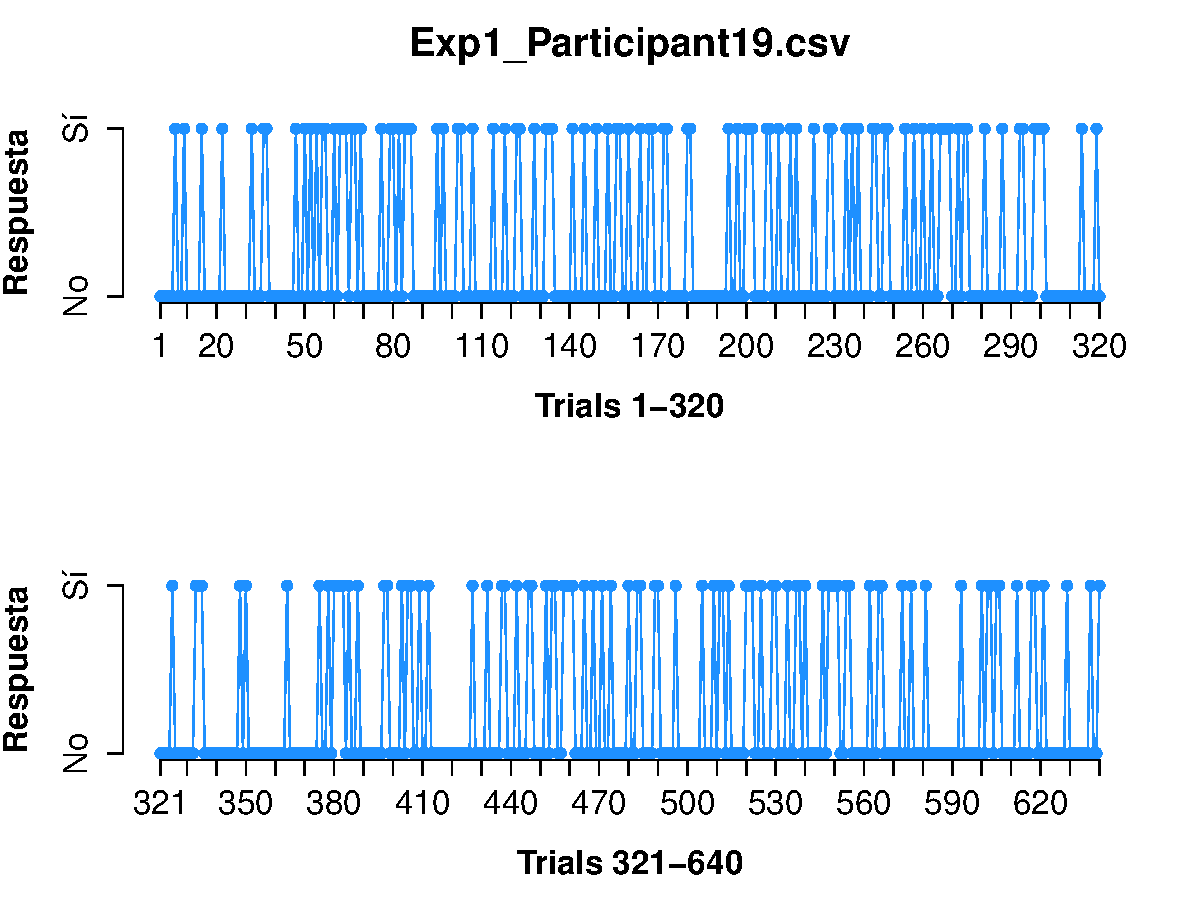
\includegraphics[width=0.30\textwidth]{Figures/Response_Exp1_P19} 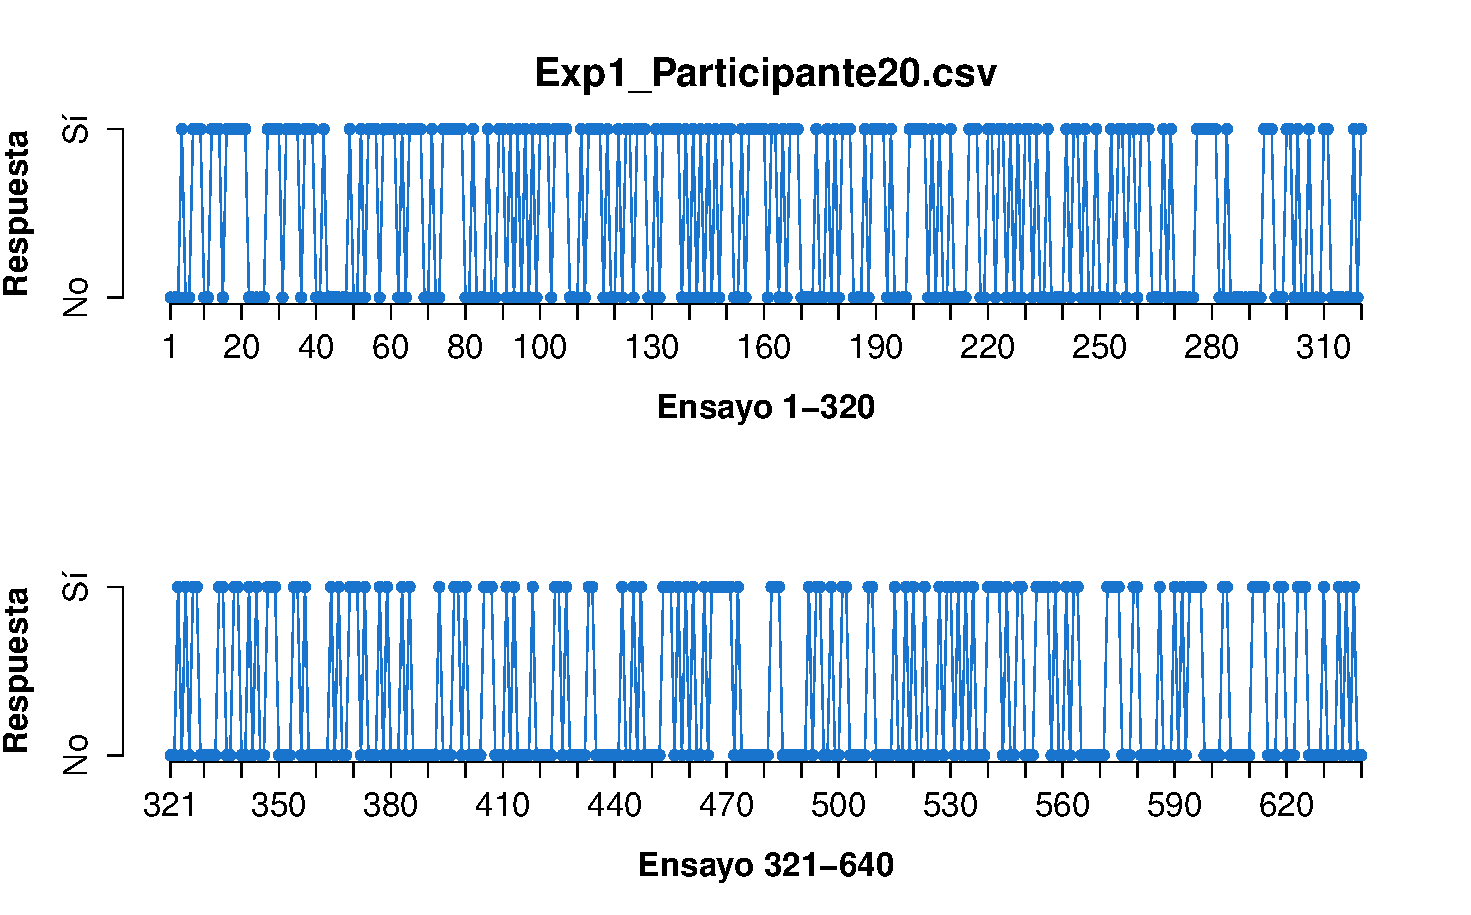
\includegraphics[width=0.30\textwidth]{Figures/Response_Exp1_P20} 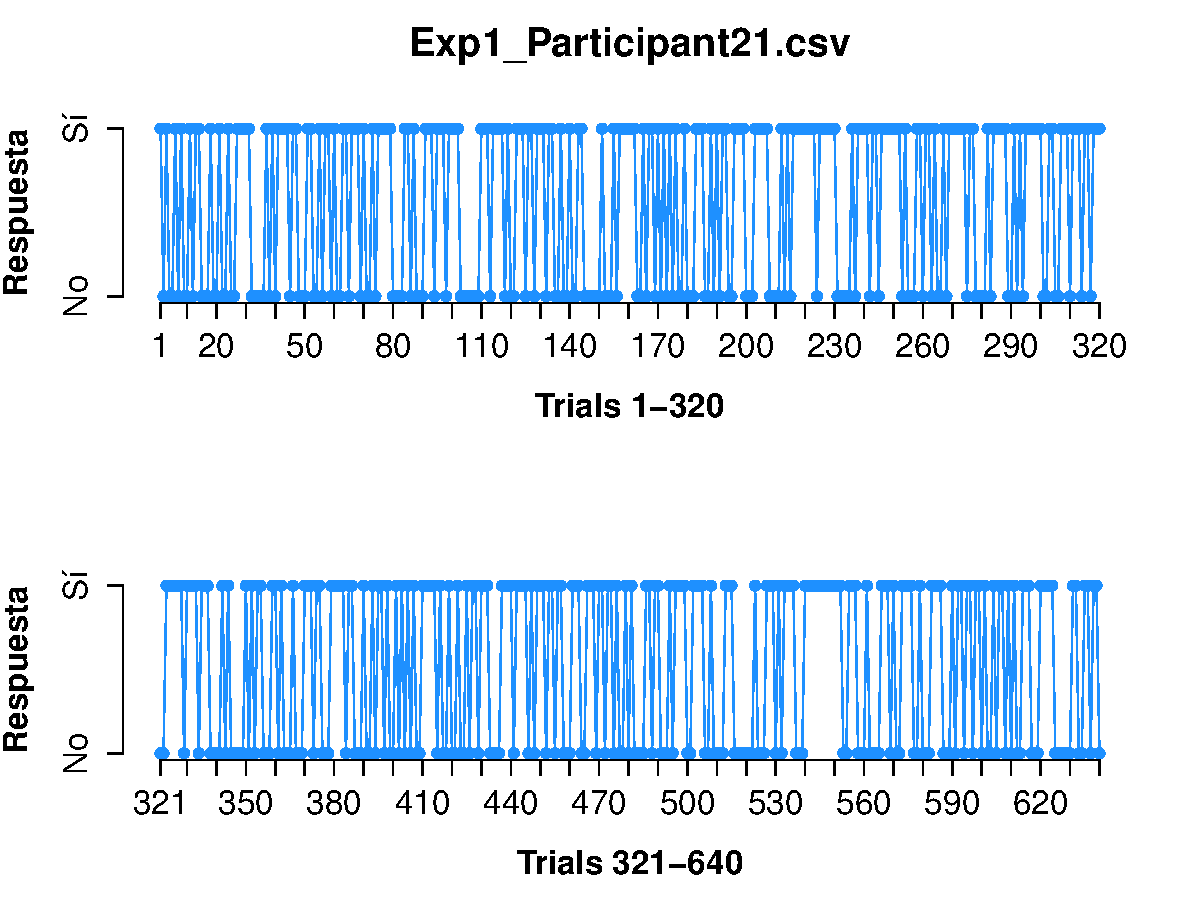
\includegraphics[width=0.30\textwidth]{Figures/Response_Exp1_P21} 
%\decoRule
\caption[Respuesta binaria registrada ensayo a ensayo; Experimento 1]{Se muestran las respuestas registradas en cada ensayo por los veintiun participantes del Experimento 1, para la tarea de detección binaria. Por cada participante se incluyen dos gráficas que presentan las respuestas emitidas en la primera y la segunda mitad del experimento, (panel superior e inferior, respectivamente).}
\label{fig:Response_E1}
\end{figure}

\begin{figure}[th]
\centering
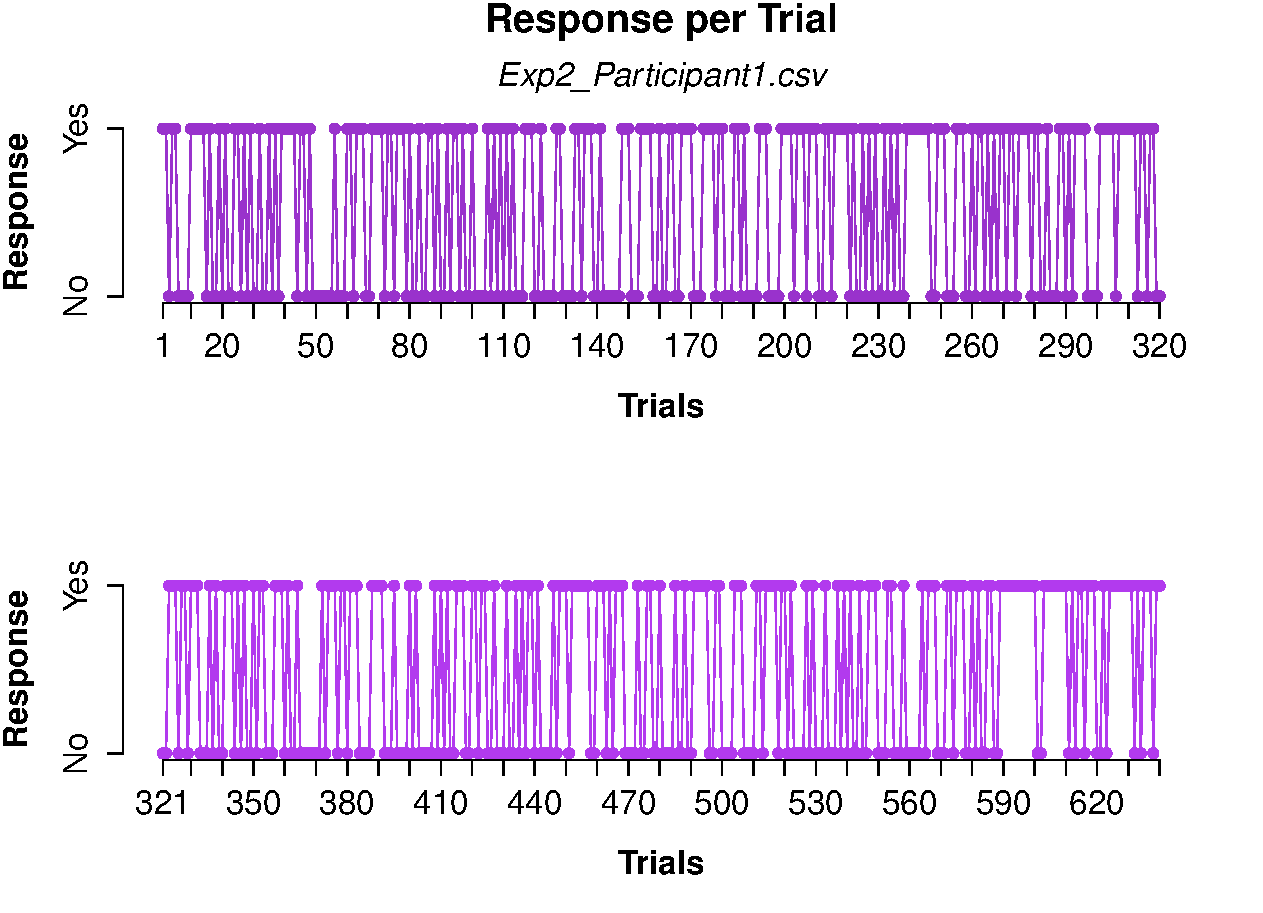
\includegraphics[width=0.30\textwidth]{Figures/Response_Exp2_P1} 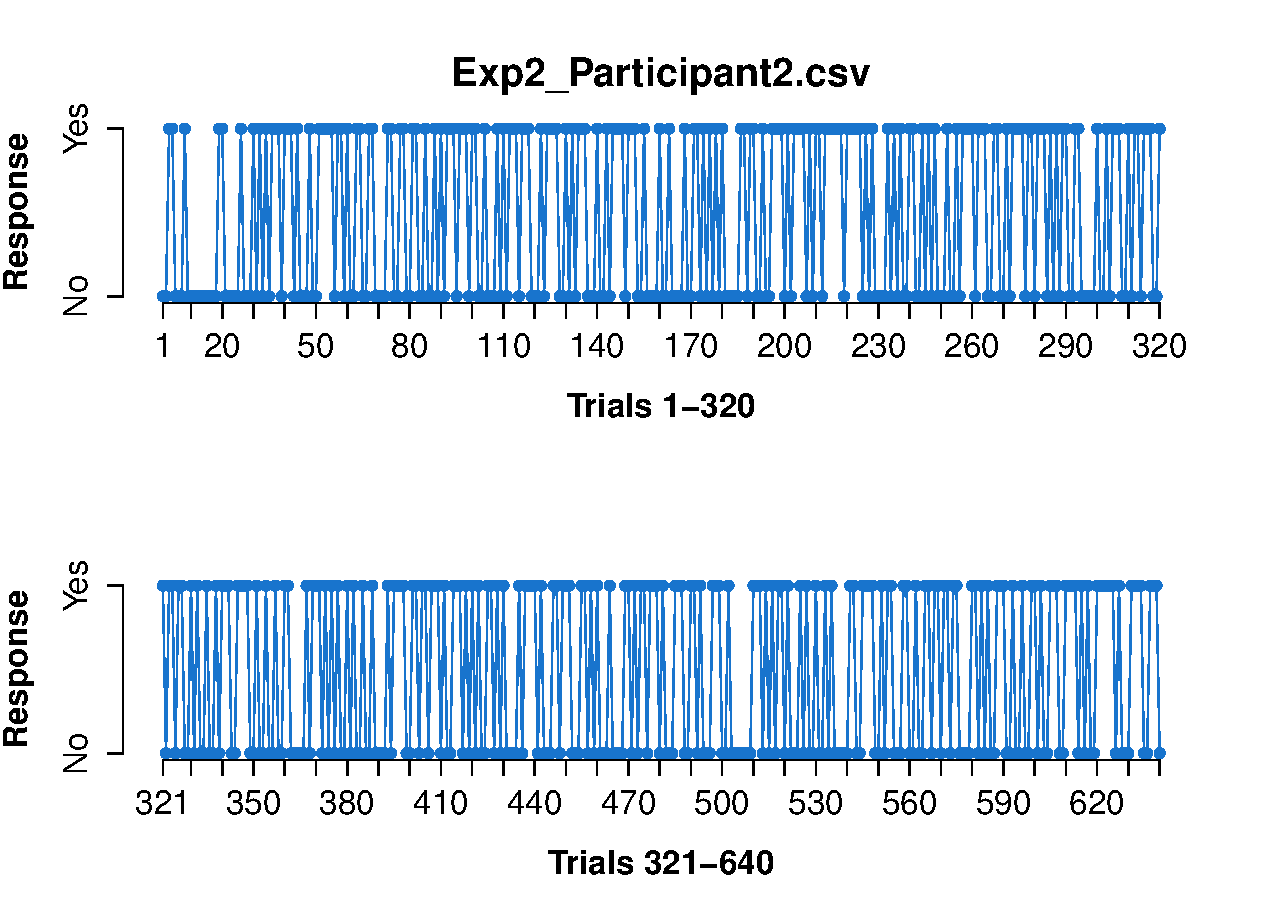
\includegraphics[width=0.30\textwidth]{Figures/Response_Exp2_P2} 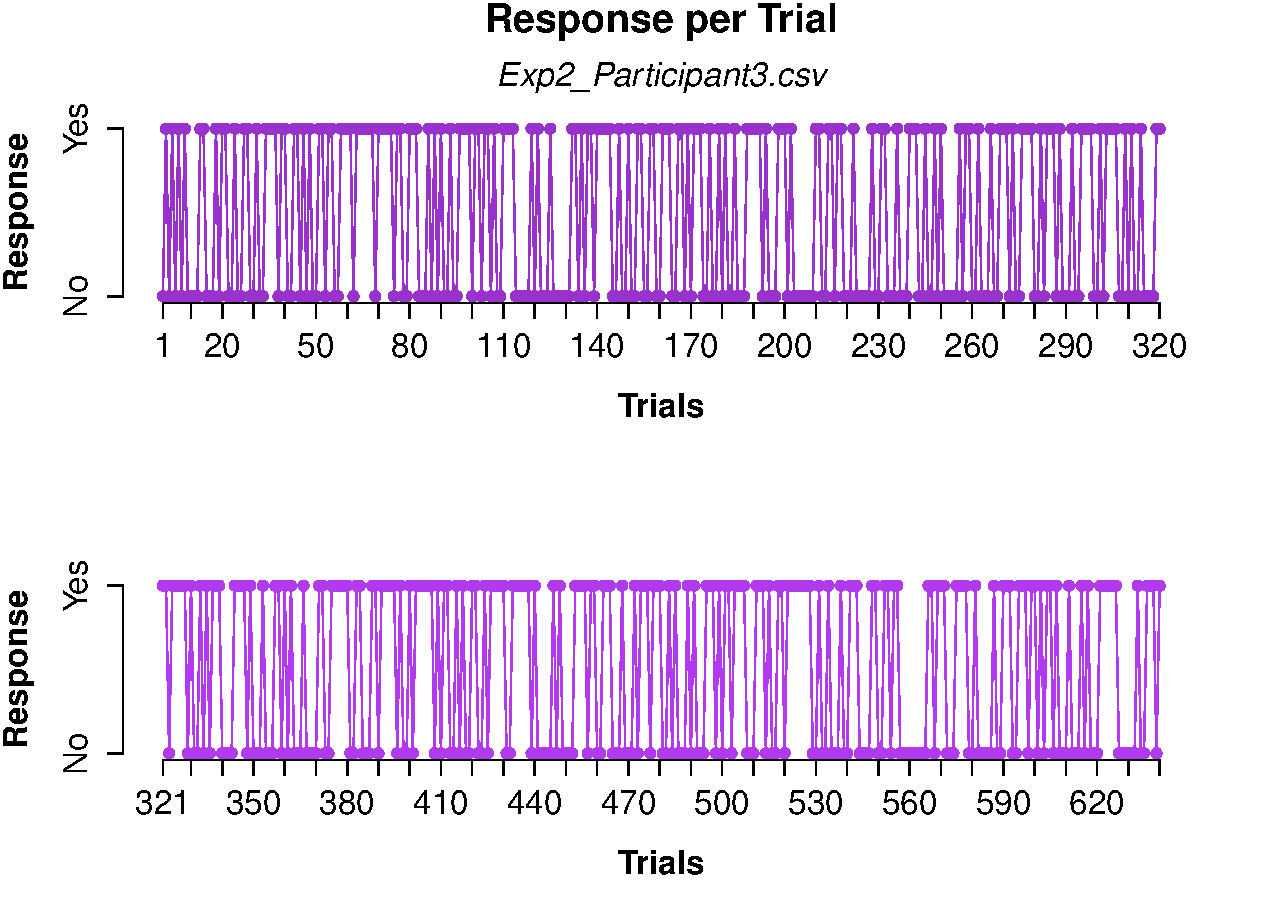
\includegraphics[width=0.30\textwidth]{Figures/Response_Exp2_P3}
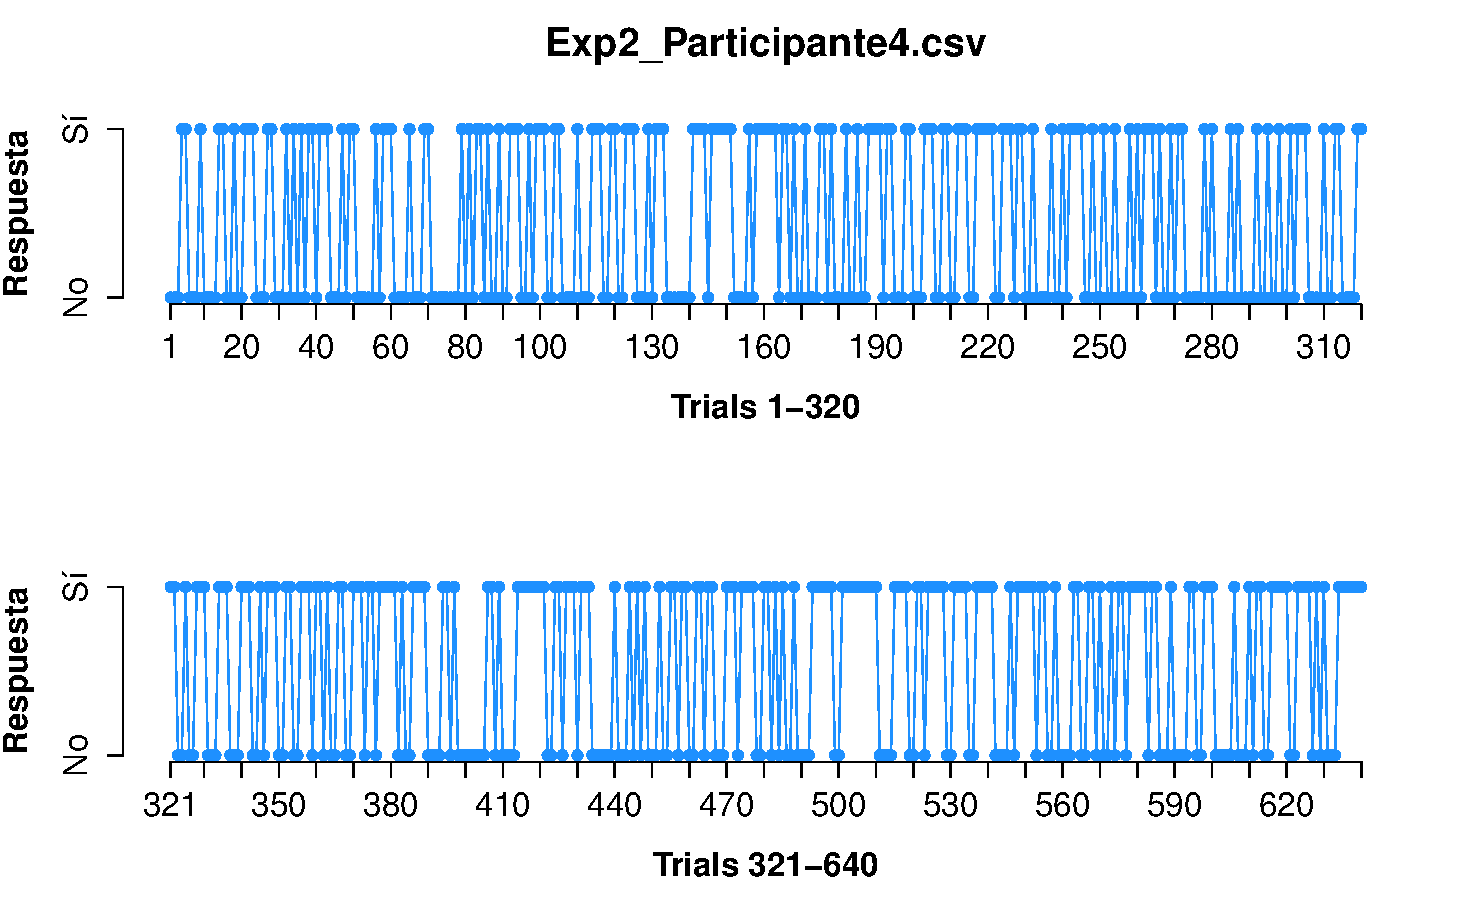
\includegraphics[width=0.30\textwidth]{Figures/Response_Exp2_P4} 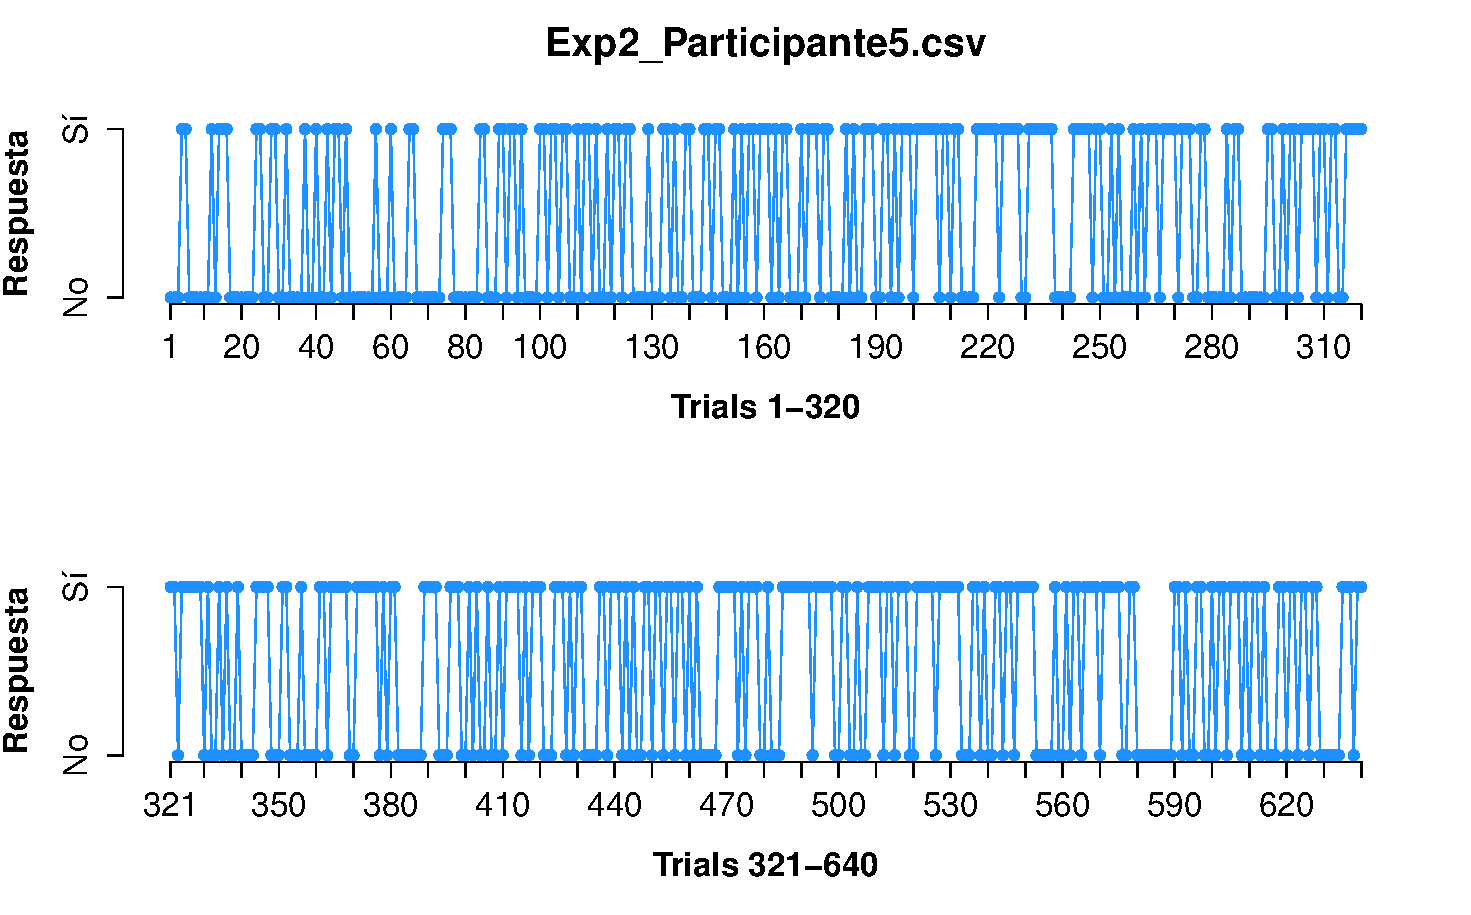
\includegraphics[width=0.30\textwidth]{Figures/Response_Exp2_P5} 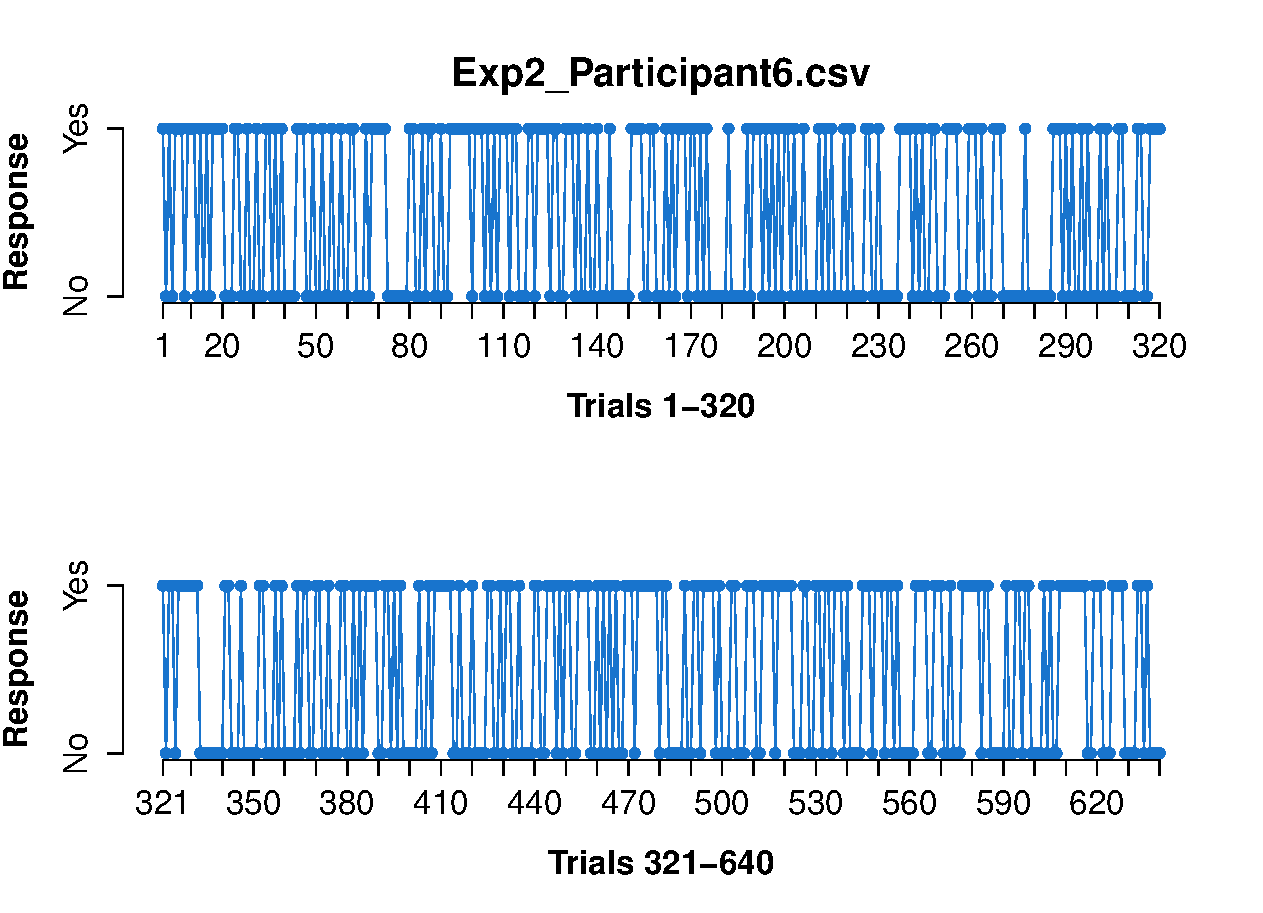
\includegraphics[width=0.30\textwidth]{Figures/Response_Exp2_P6}
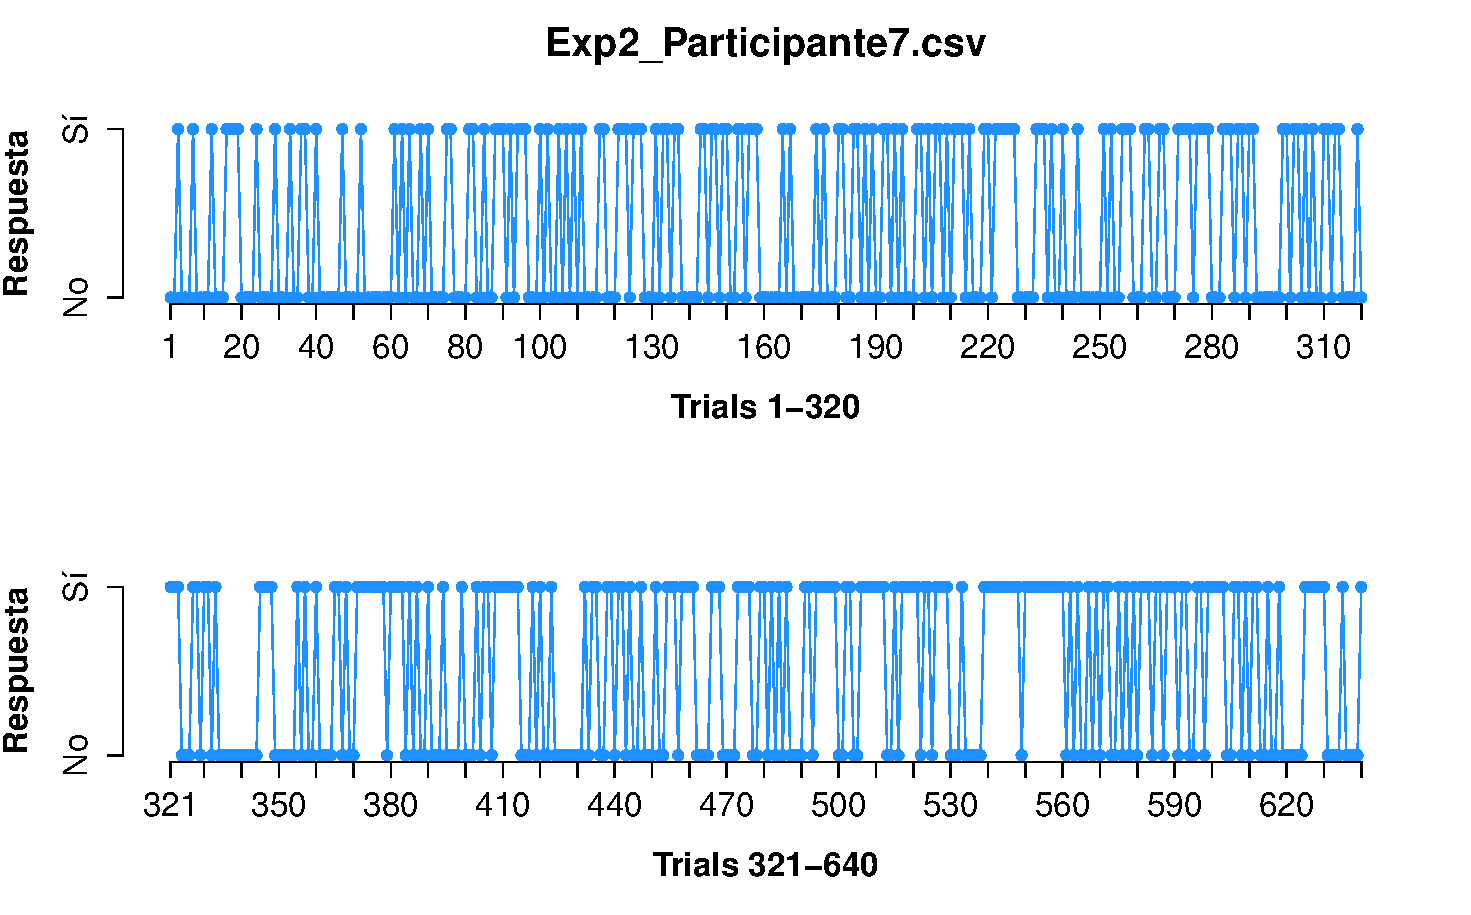
\includegraphics[width=0.30\textwidth]{Figures/Response_Exp2_P7} 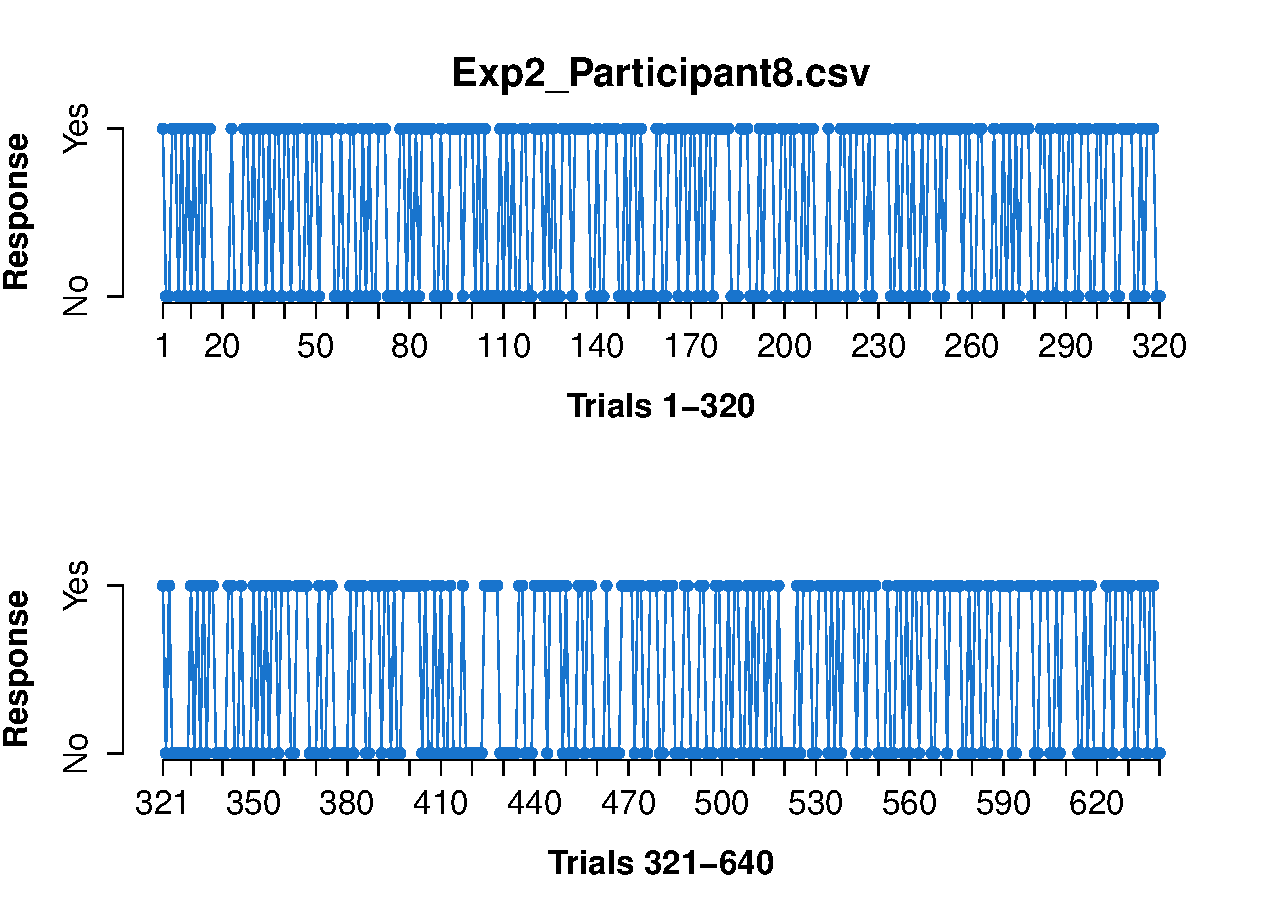
\includegraphics[width=0.30\textwidth]{Figures/Response_Exp2_P8} 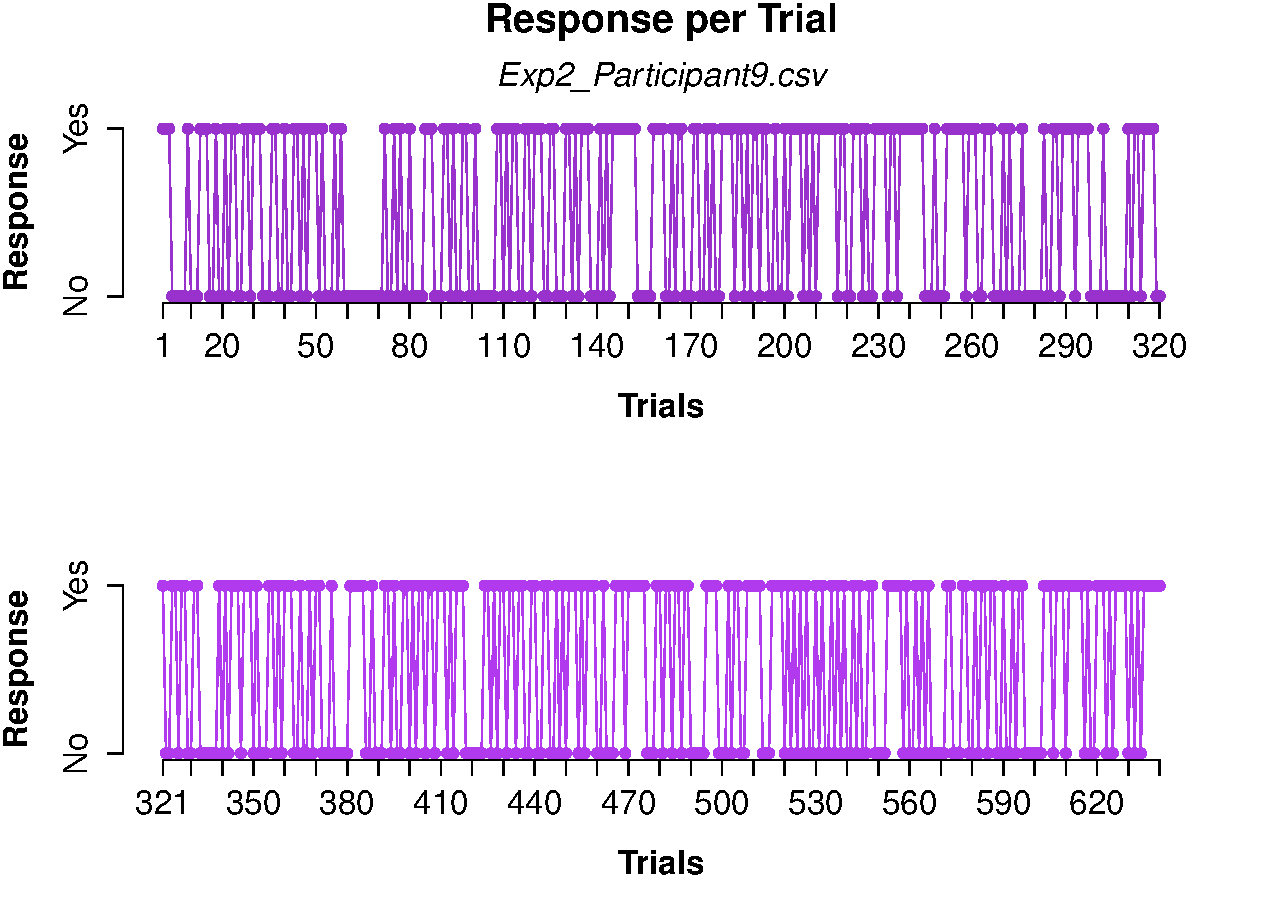
\includegraphics[width=0.30\textwidth]{Figures/Response_Exp2_P9}
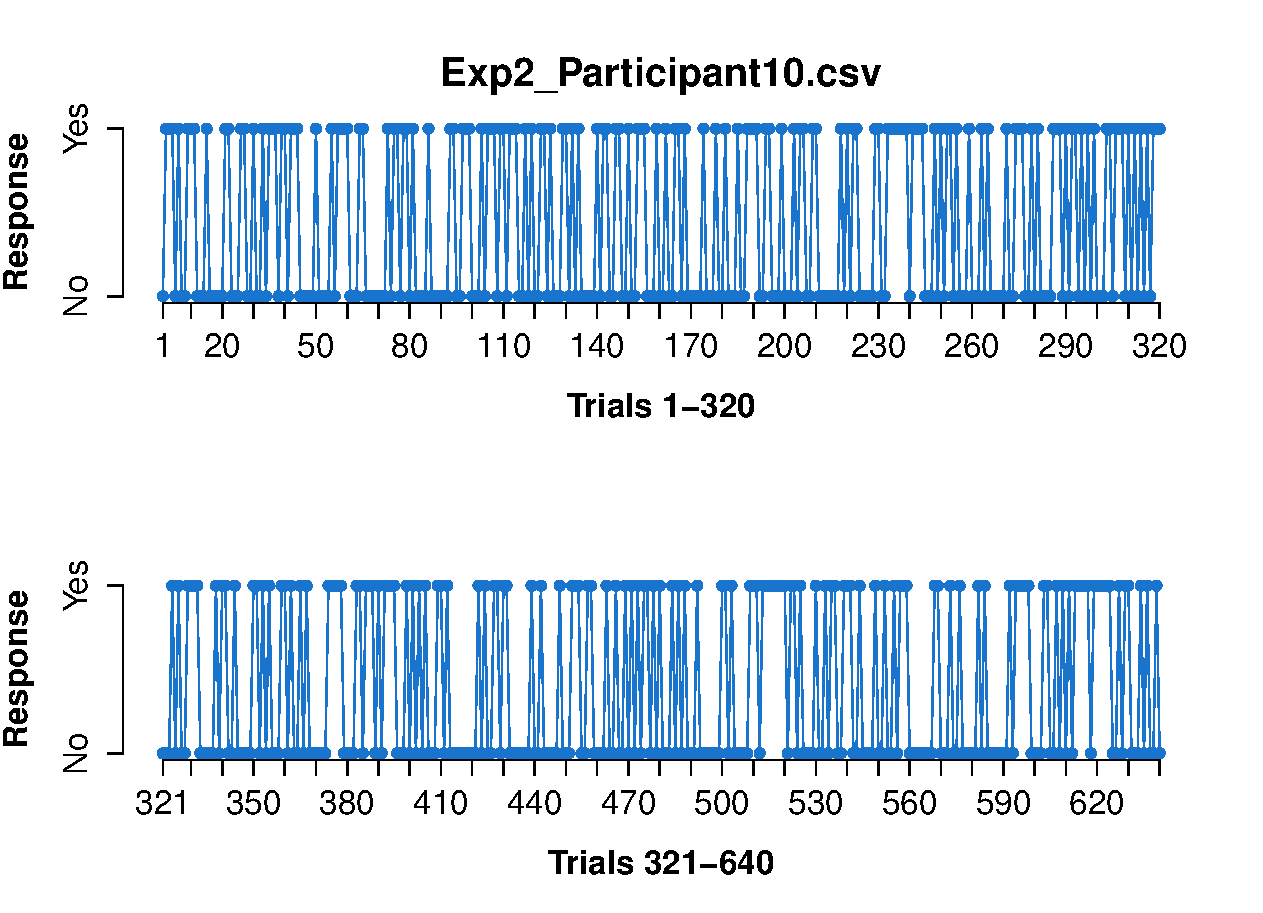
\includegraphics[width=0.30\textwidth]{Figures/Response_Exp2_P10} 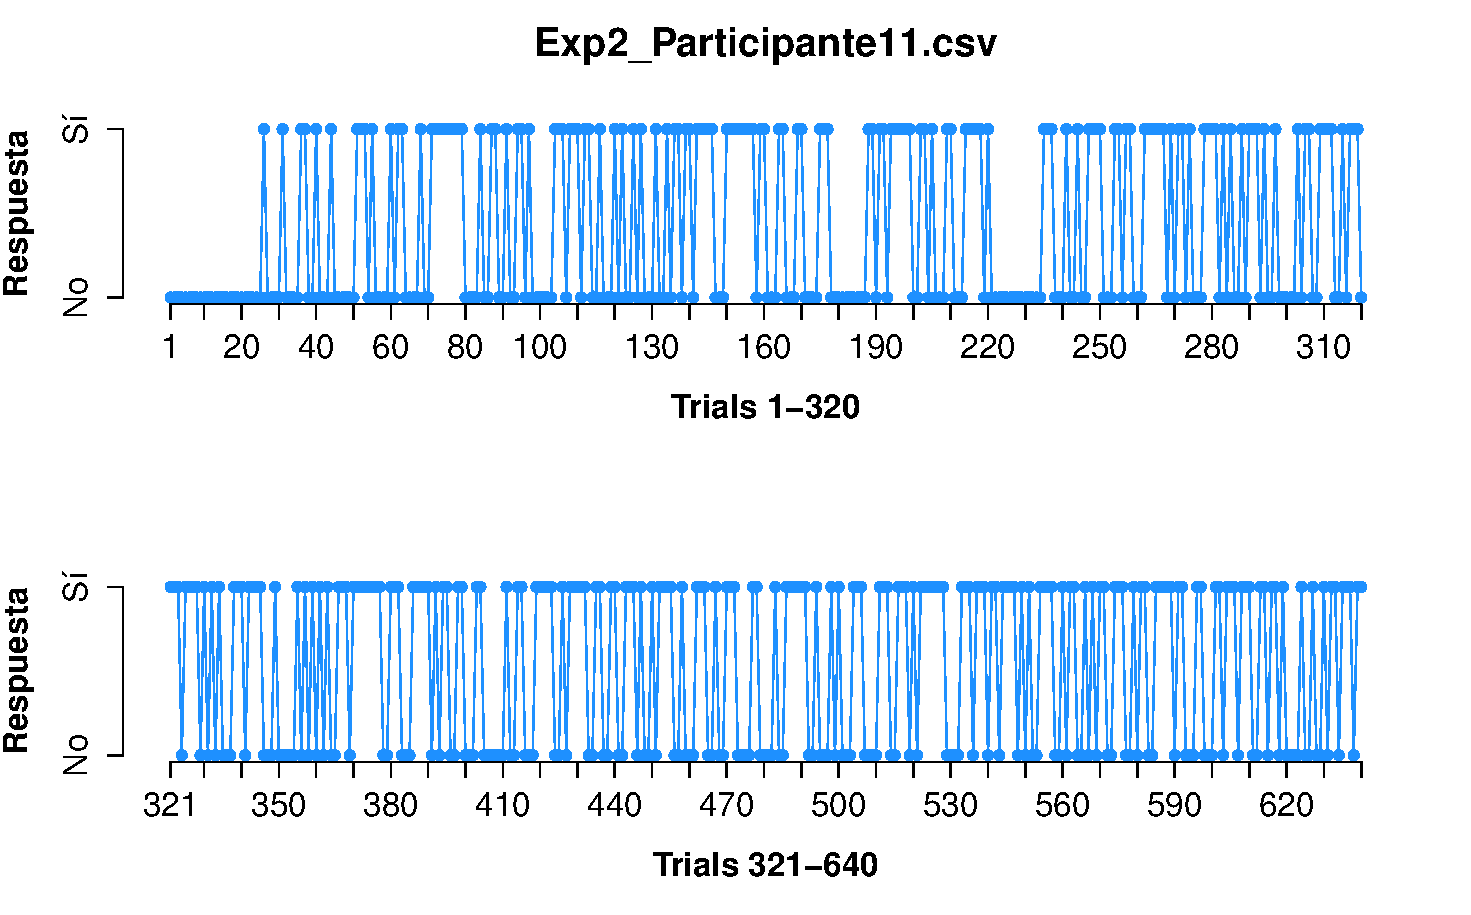
\includegraphics[width=0.30\textwidth]{Figures/Response_Exp2_P11} 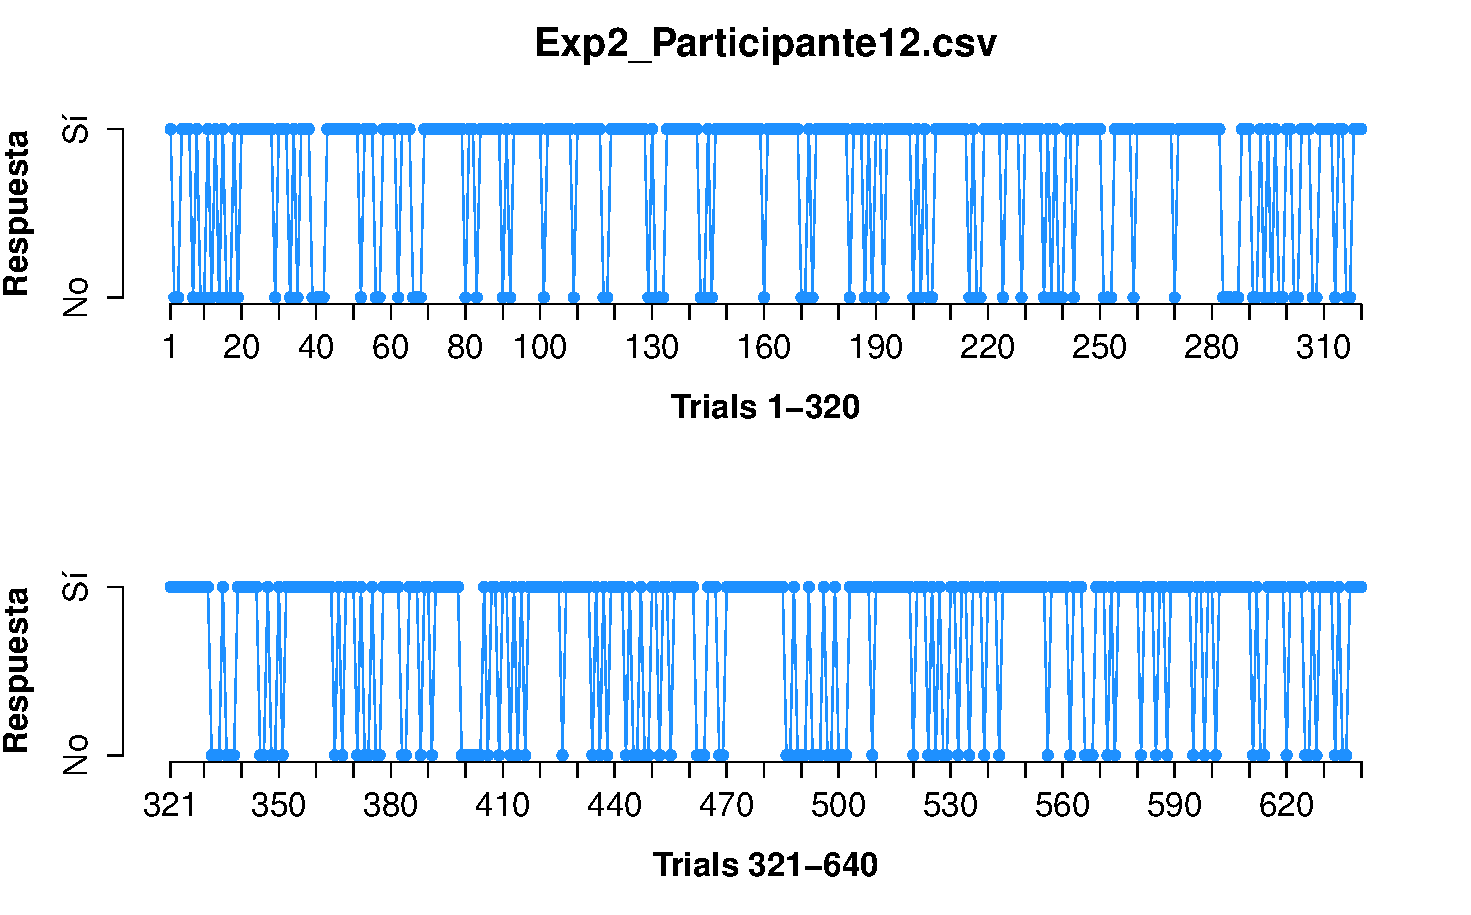
\includegraphics[width=0.30\textwidth]{Figures/Response_Exp2_P12}
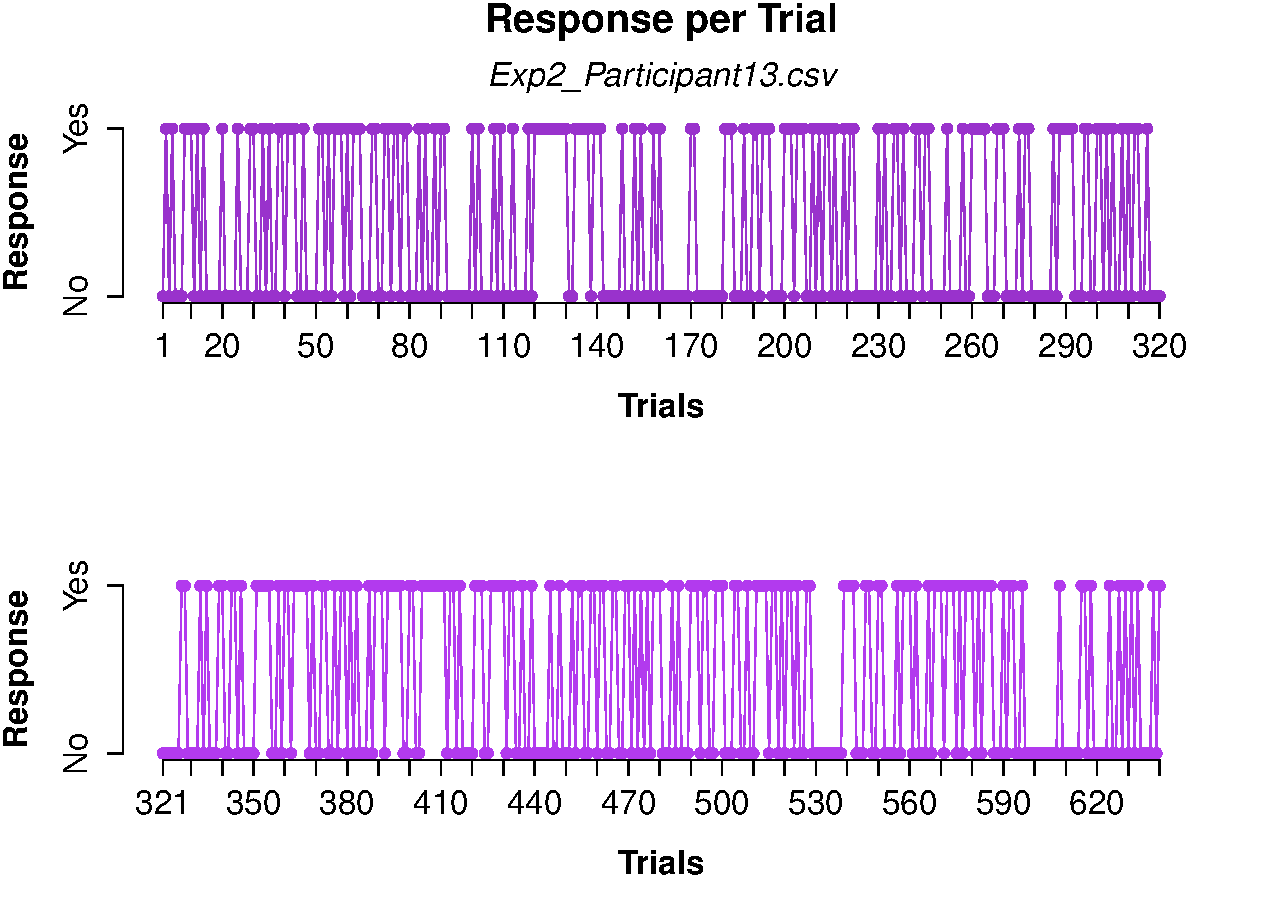
\includegraphics[width=0.30\textwidth]{Figures/Response_Exp2_P13} 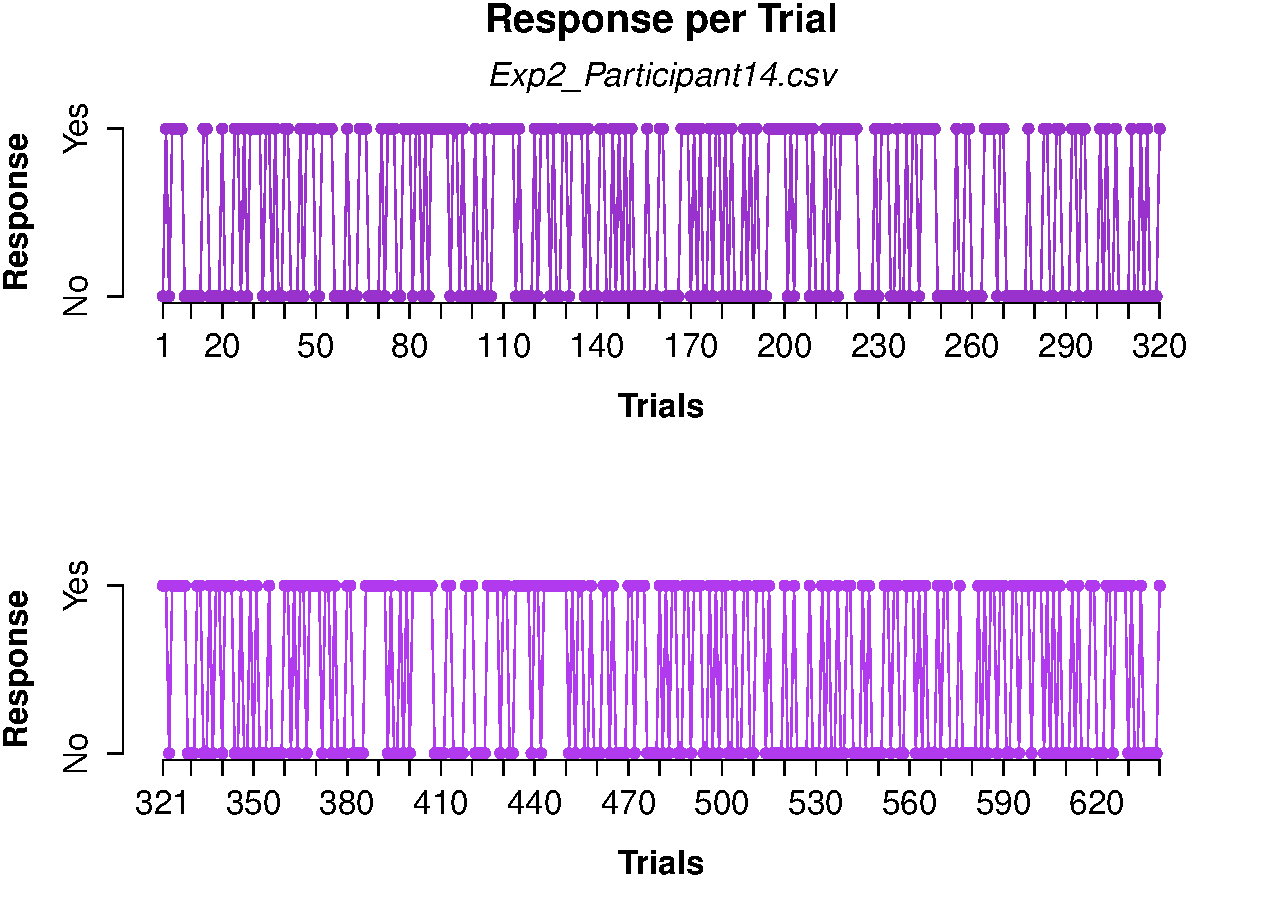
\includegraphics[width=0.30\textwidth]{Figures/Response_Exp2_P14} 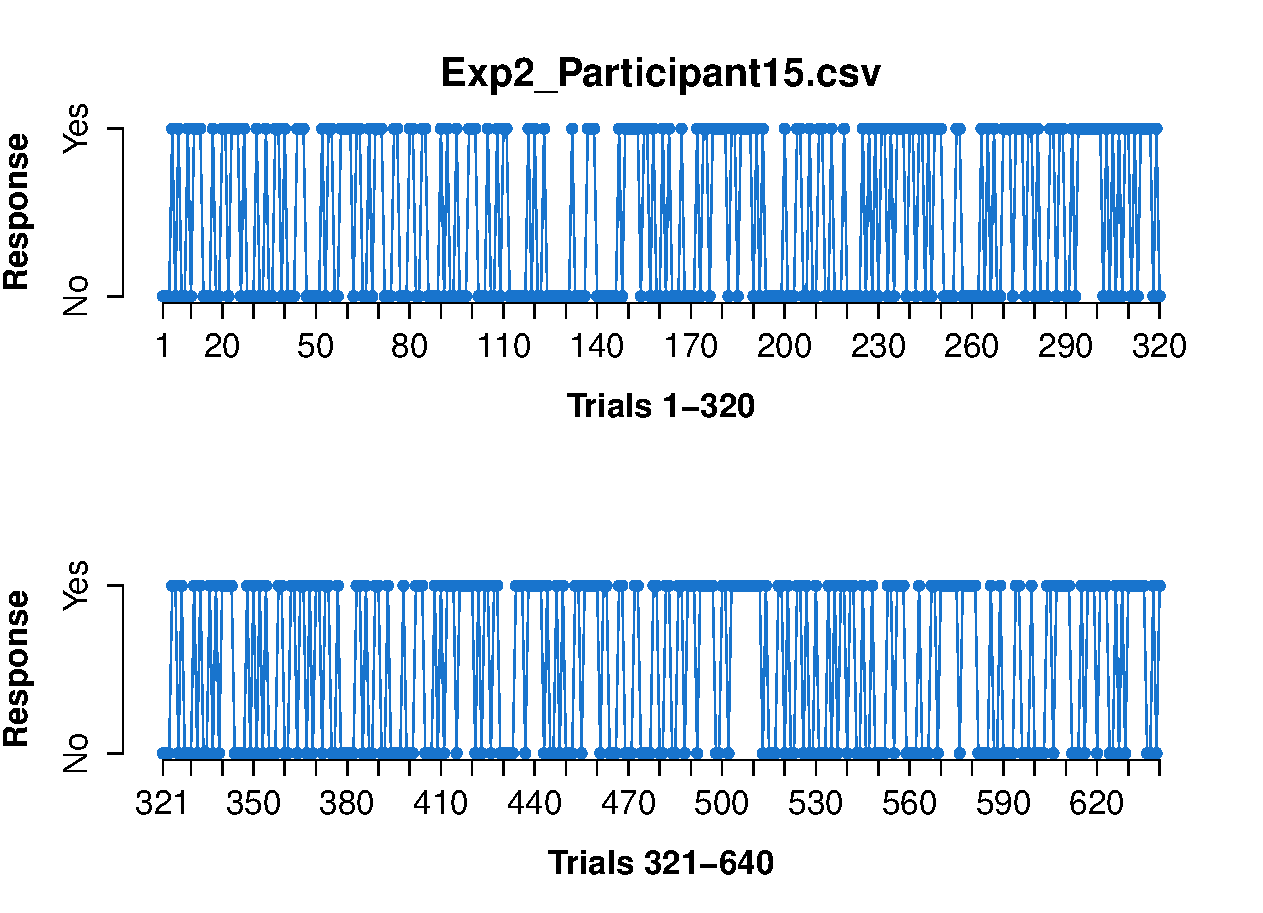
\includegraphics[width=0.30\textwidth]{Figures/Response_Exp2_P15}
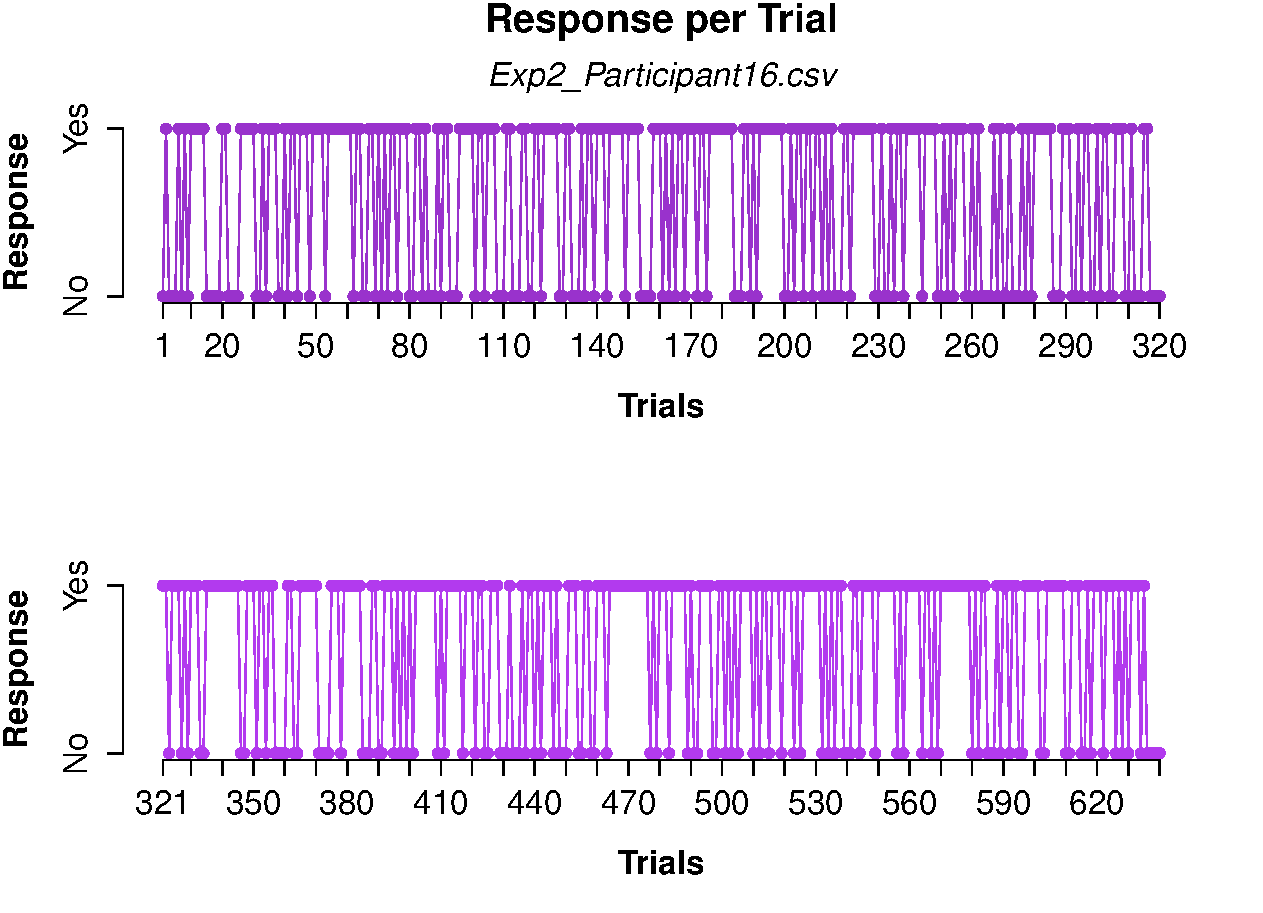
\includegraphics[width=0.30\textwidth]{Figures/Response_Exp2_P16} 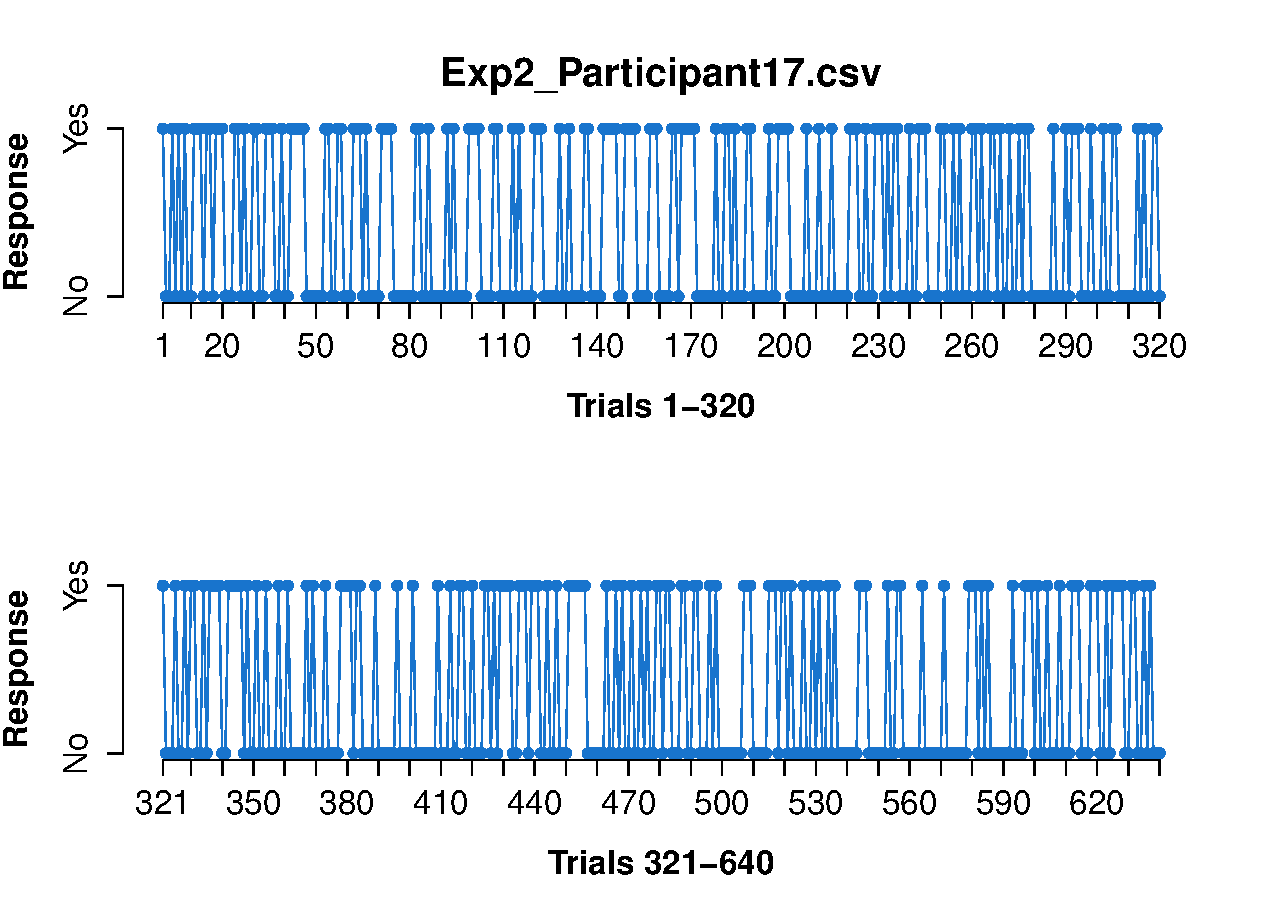
\includegraphics[width=0.30\textwidth]{Figures/Response_Exp2_P17} 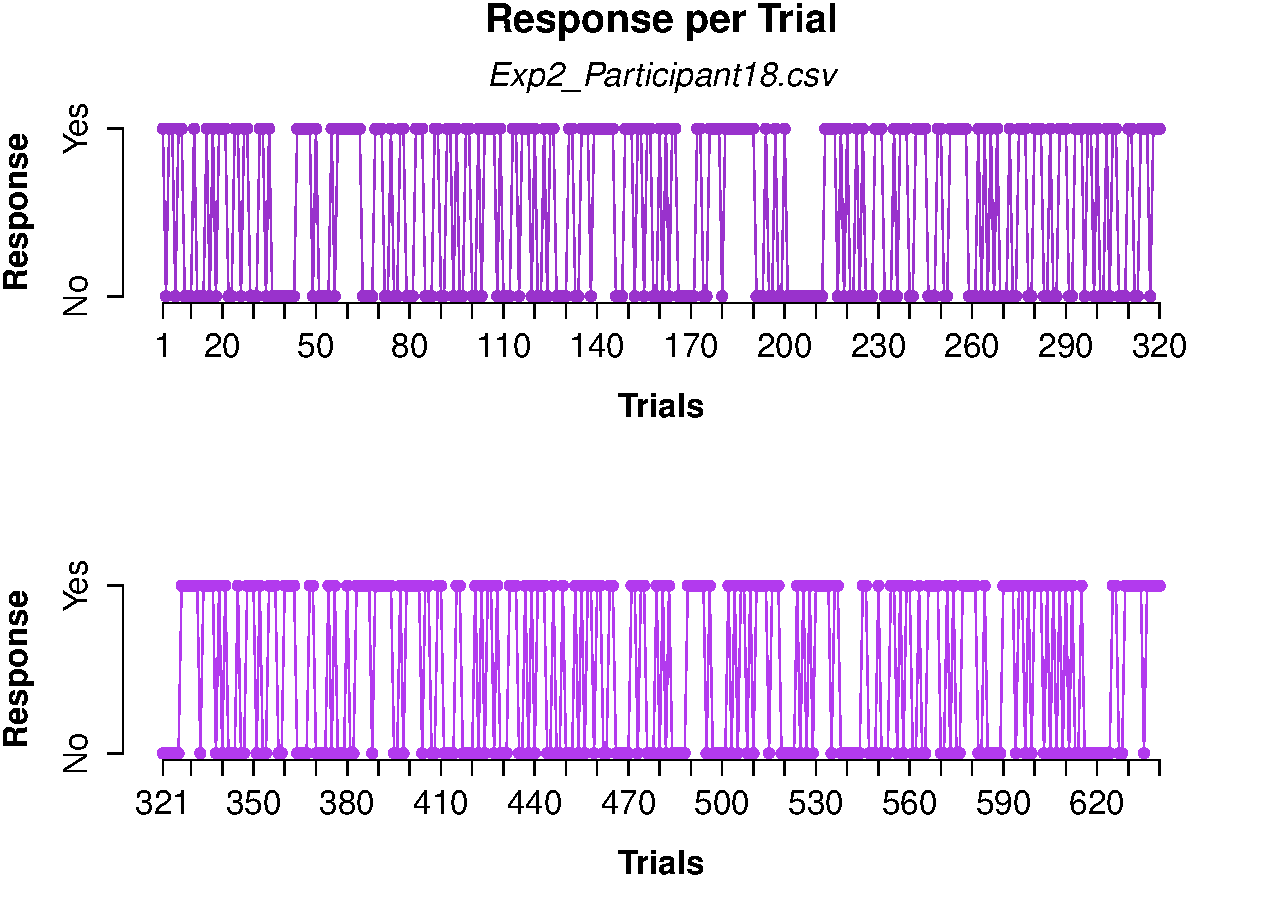
\includegraphics[width=0.30\textwidth]{Figures/Response_Exp2_P18}
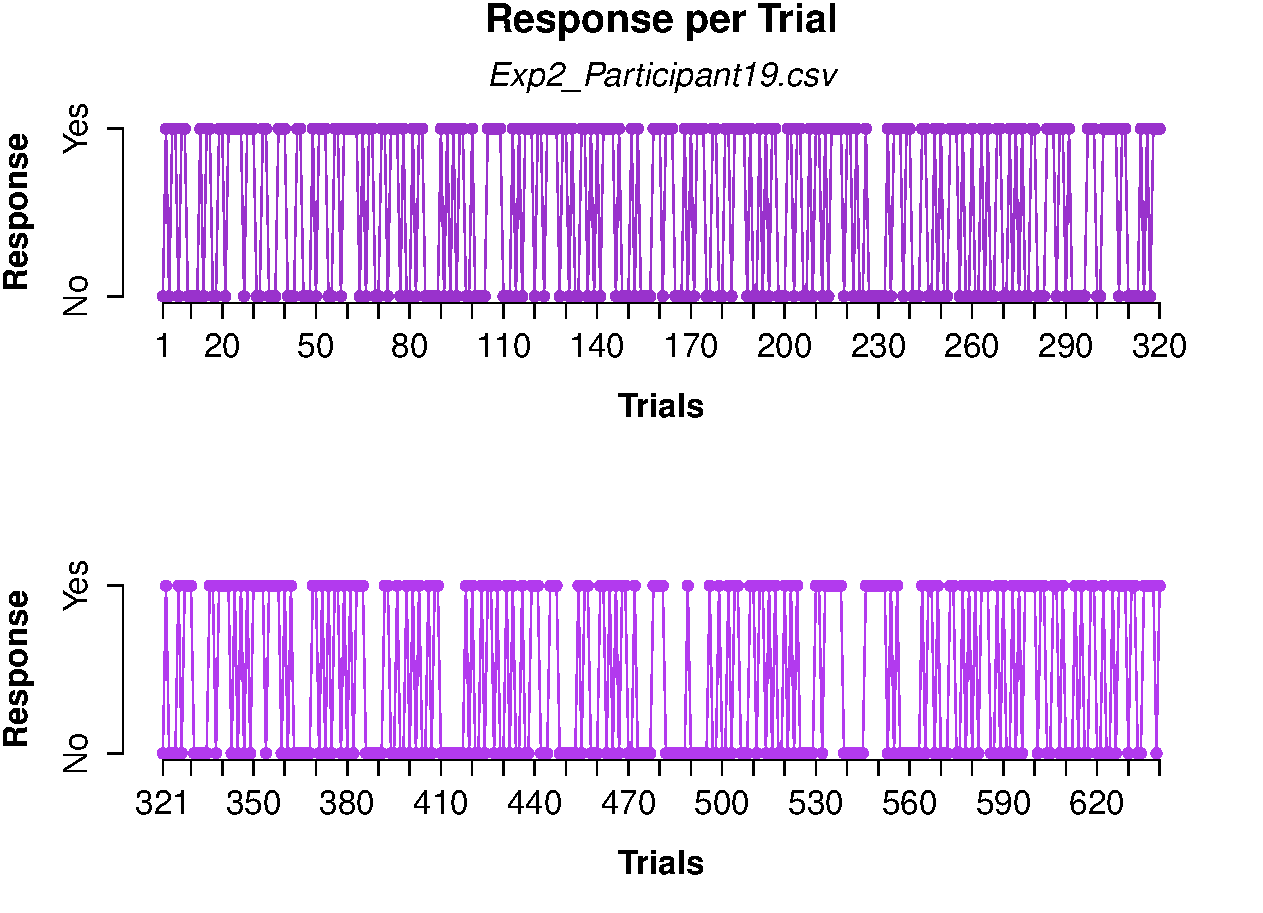
\includegraphics[width=0.30\textwidth]{Figures/Response_Exp2_P19} 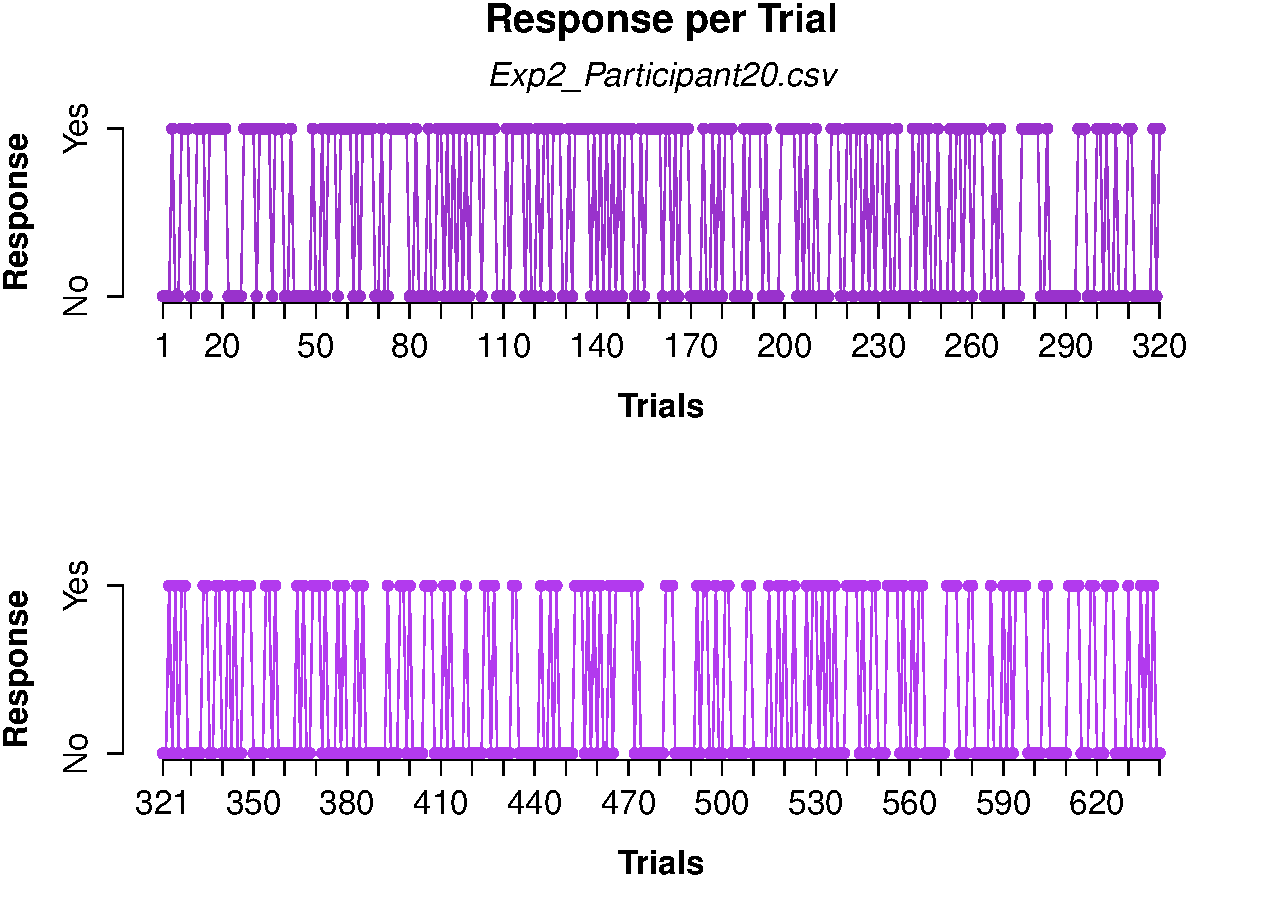
\includegraphics[width=0.30\textwidth]{Figures/Response_Exp2_P20} 
%\decoRule
\caption[Respuesta binaria registrada ensayo a ensayo; Experimento 2]{Se muestran las respuestas registradas a la tarea de detección binaria en cada ensayo por cada uno de los veinte participantes del Experimento 2. Las elecciones por participante se muestran en dos páneles que corresponden a los primeros y los últimos 320 ensayos del experimento (panel superior e inferior, respectivamente).}
\label{fig:Response_E2}
\end{figure}

\begin{figure}[th]
\centering
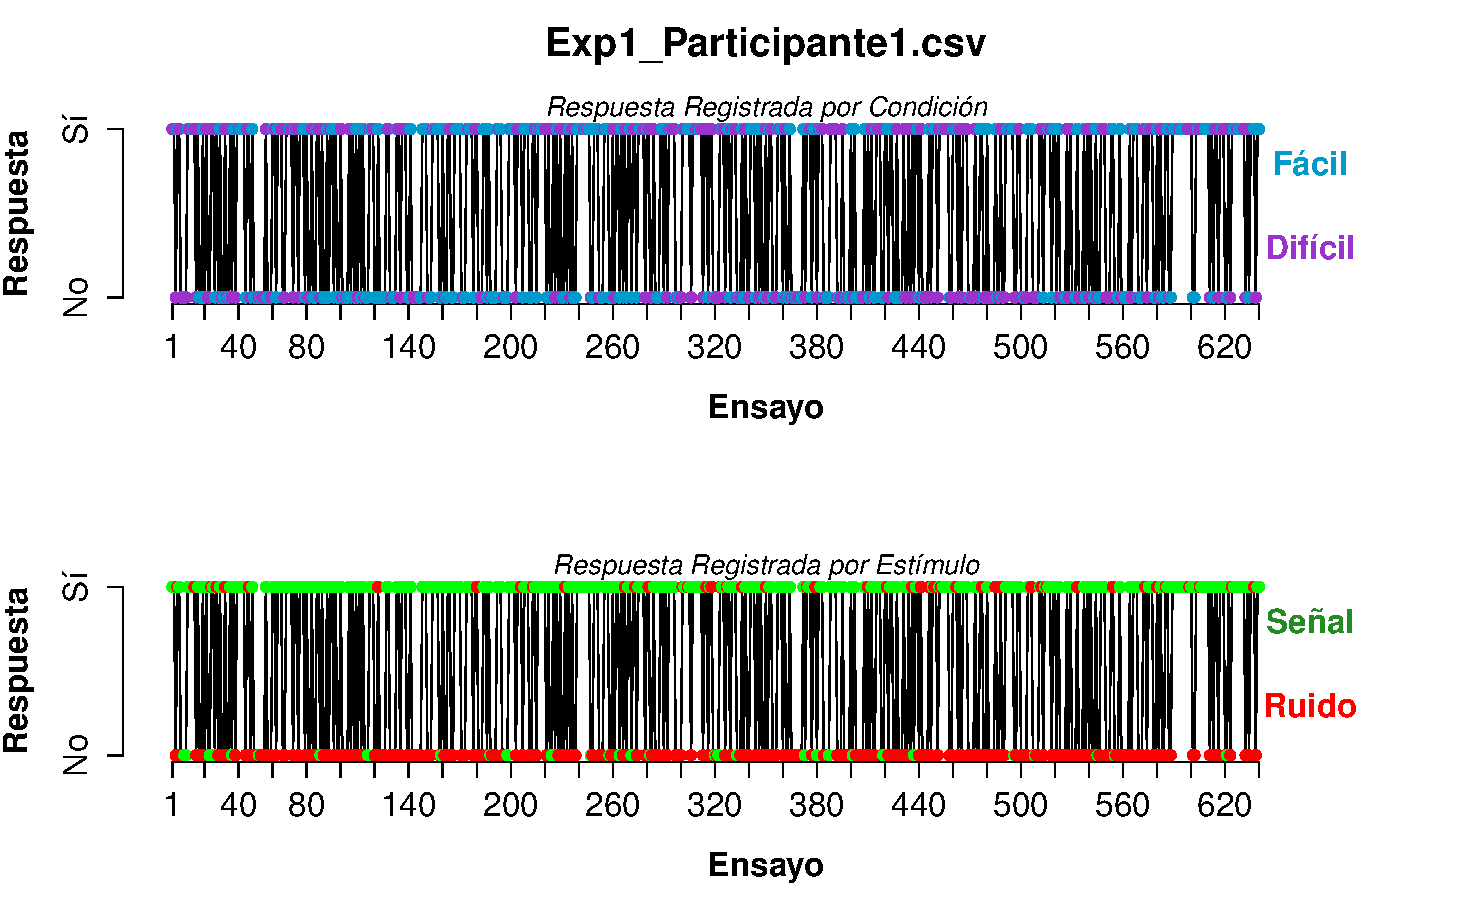
\includegraphics[width=0.30\textwidth]{Figures/BiasResp_Exp1_P1} 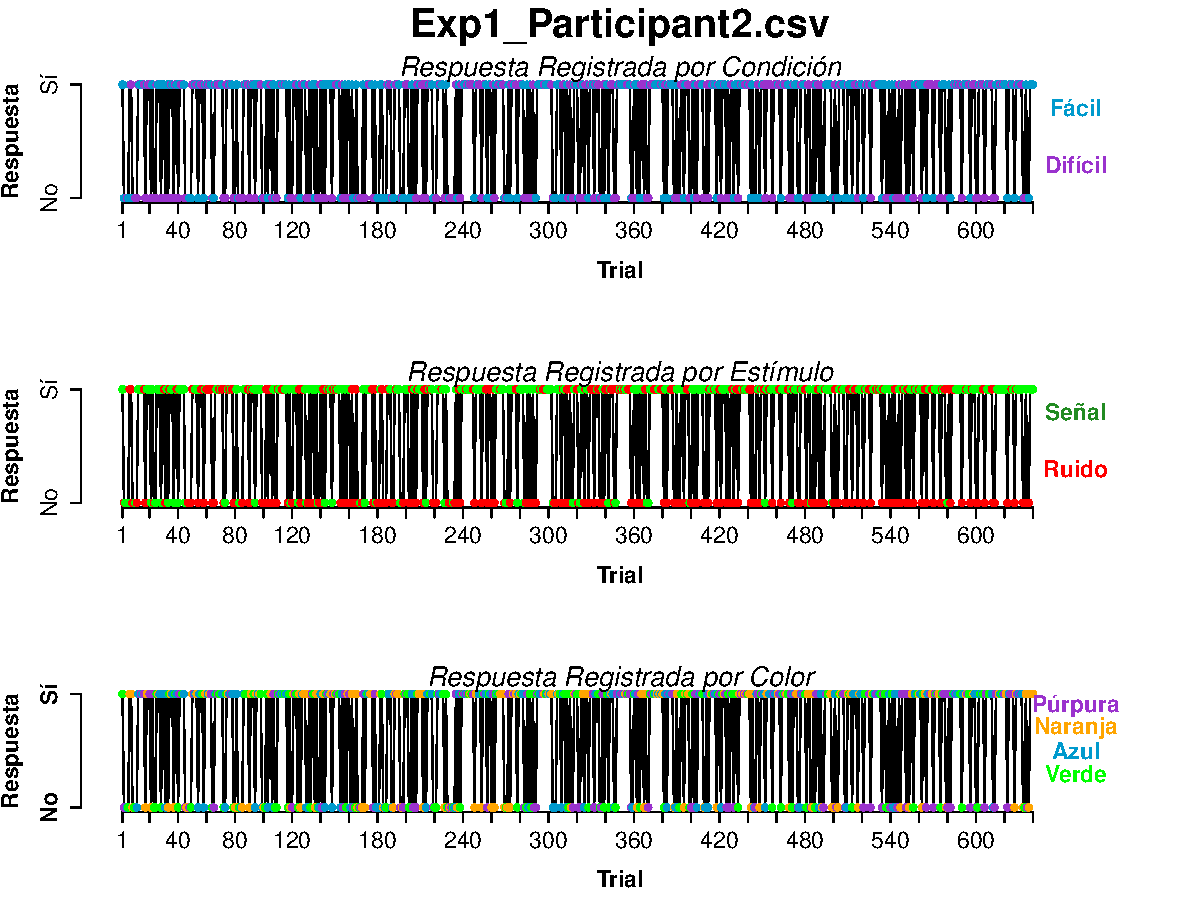
\includegraphics[width=0.30\textwidth]{Figures/BiasResp_Exp1_P2} 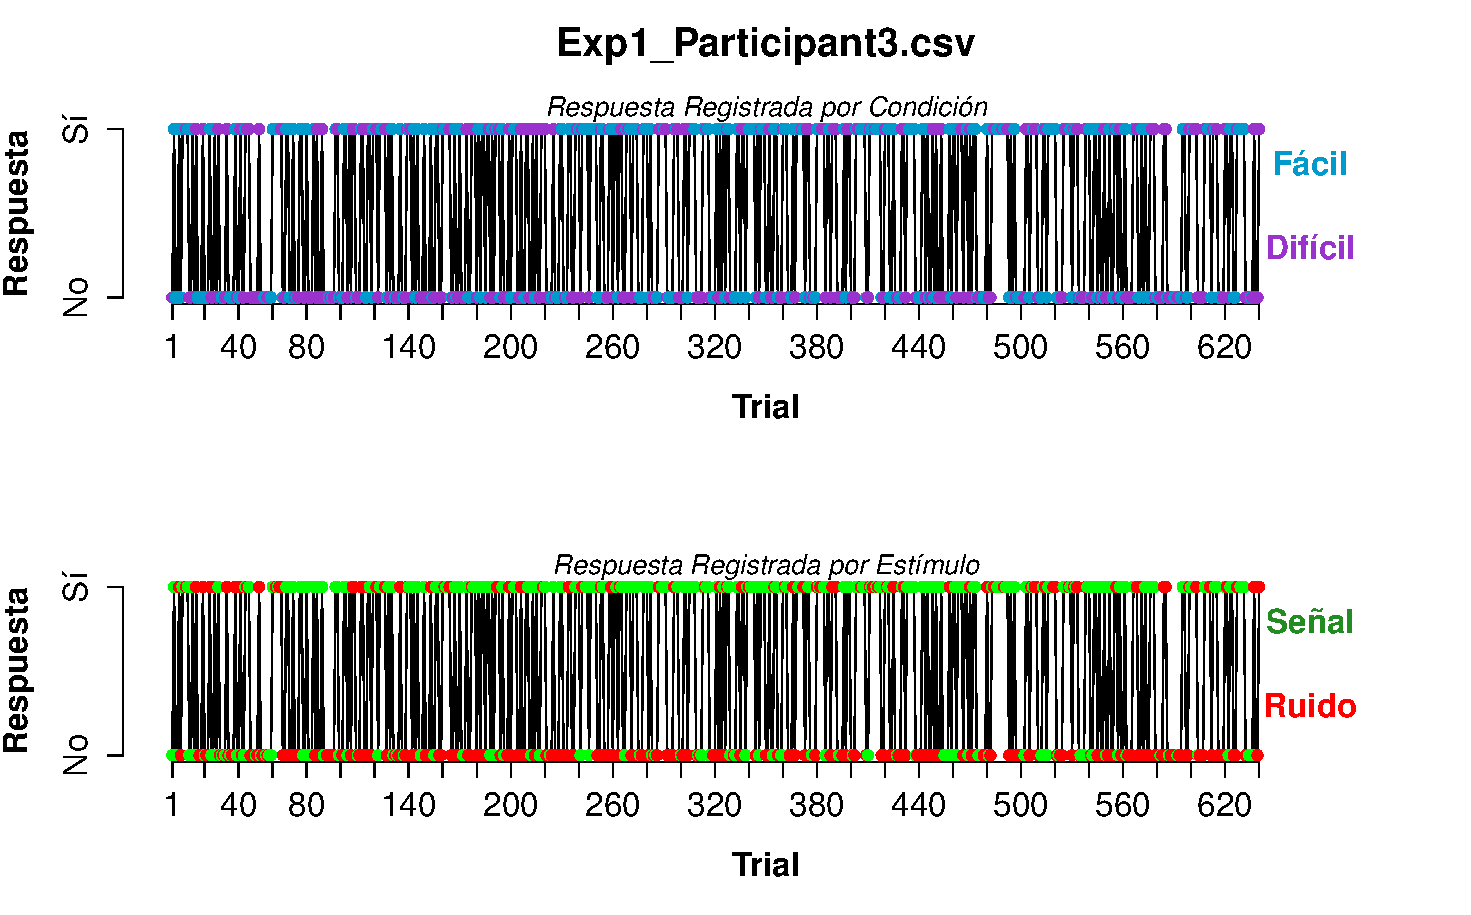
\includegraphics[width=0.30\textwidth]{Figures/BiasResp_Exp1_P3}
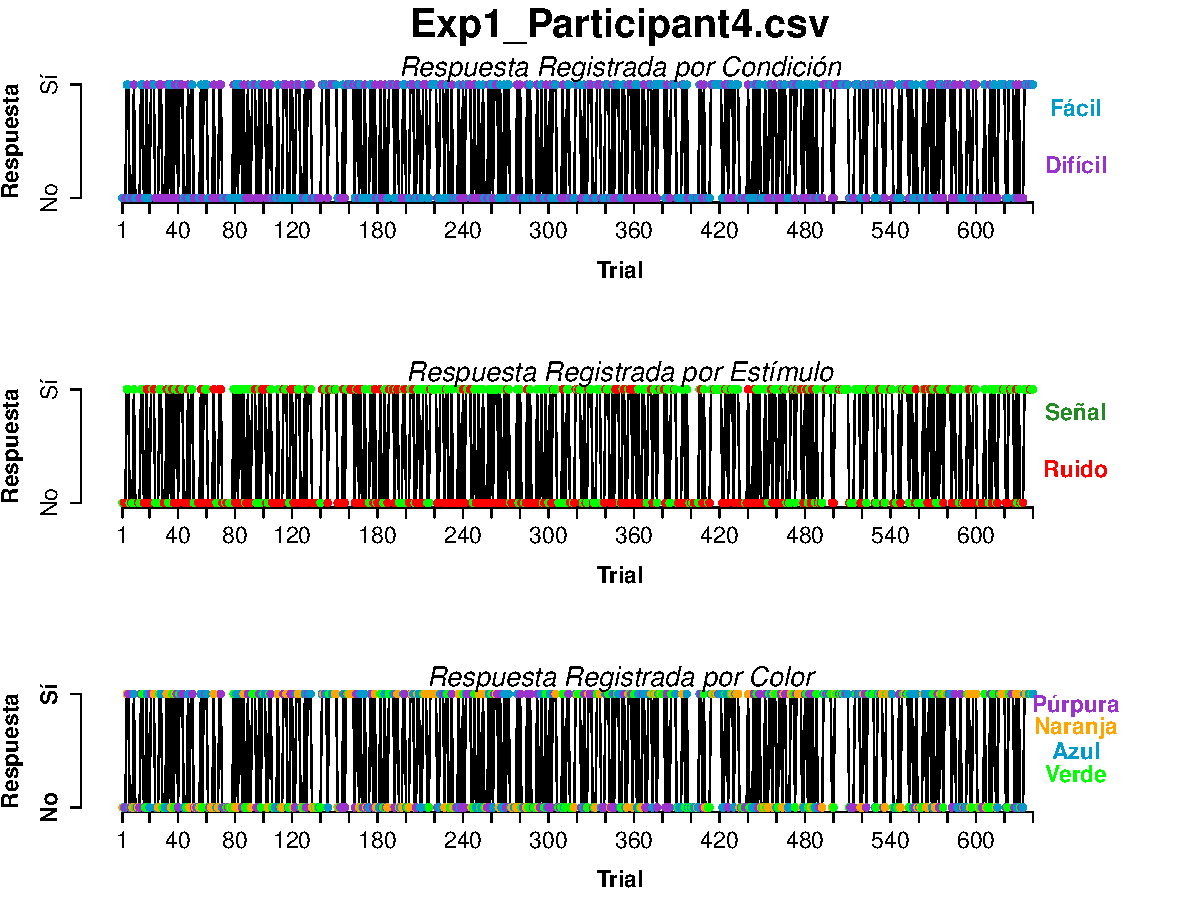
\includegraphics[width=0.30\textwidth]{Figures/BiasResp_Exp1_P4} 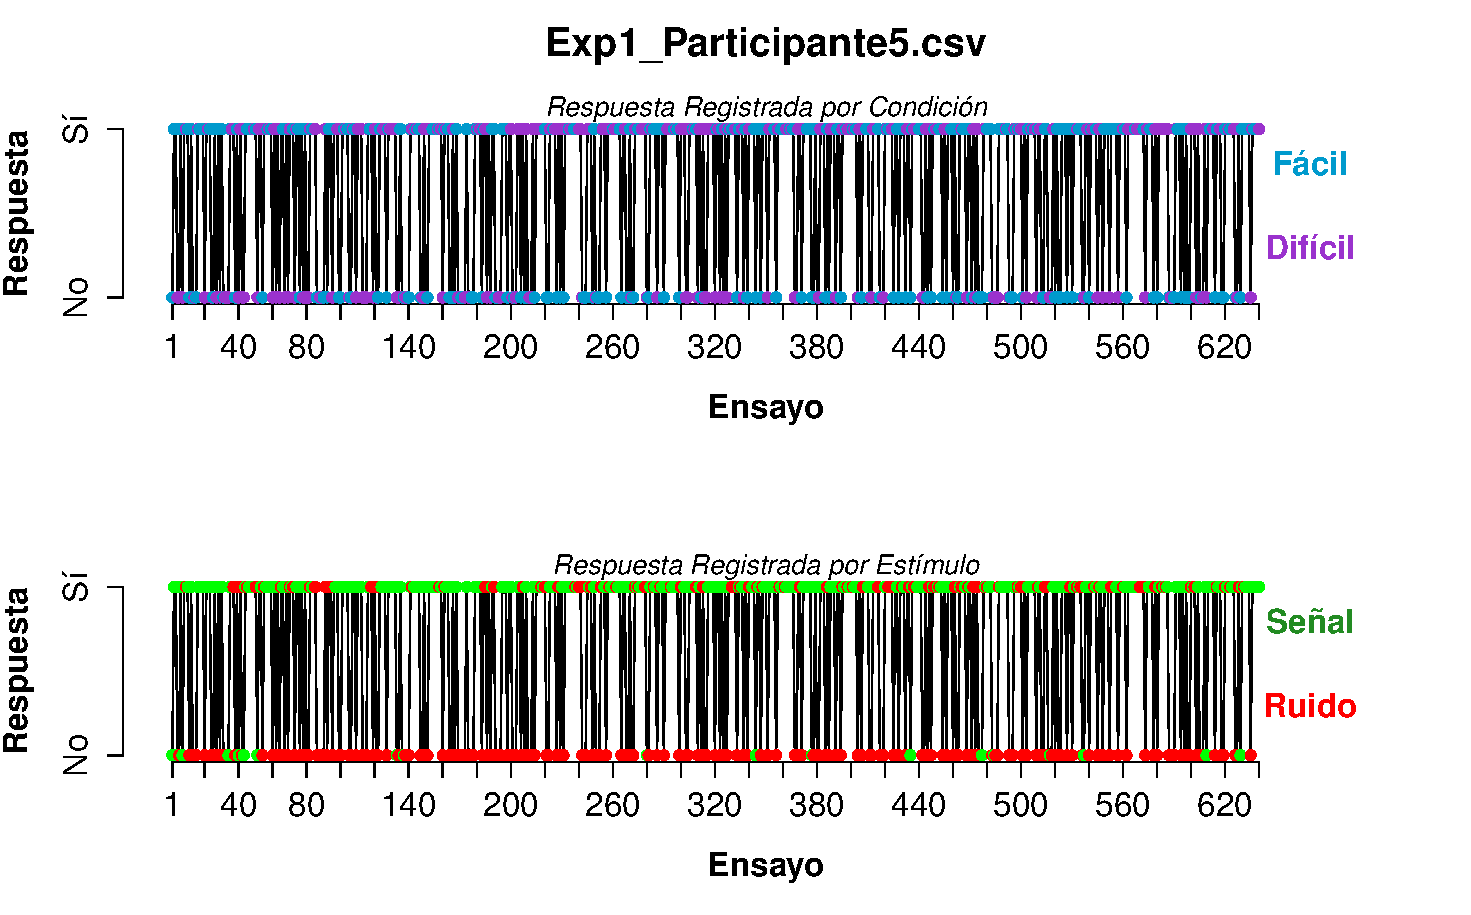
\includegraphics[width=0.30\textwidth]{Figures/BiasResp_Exp1_P5} 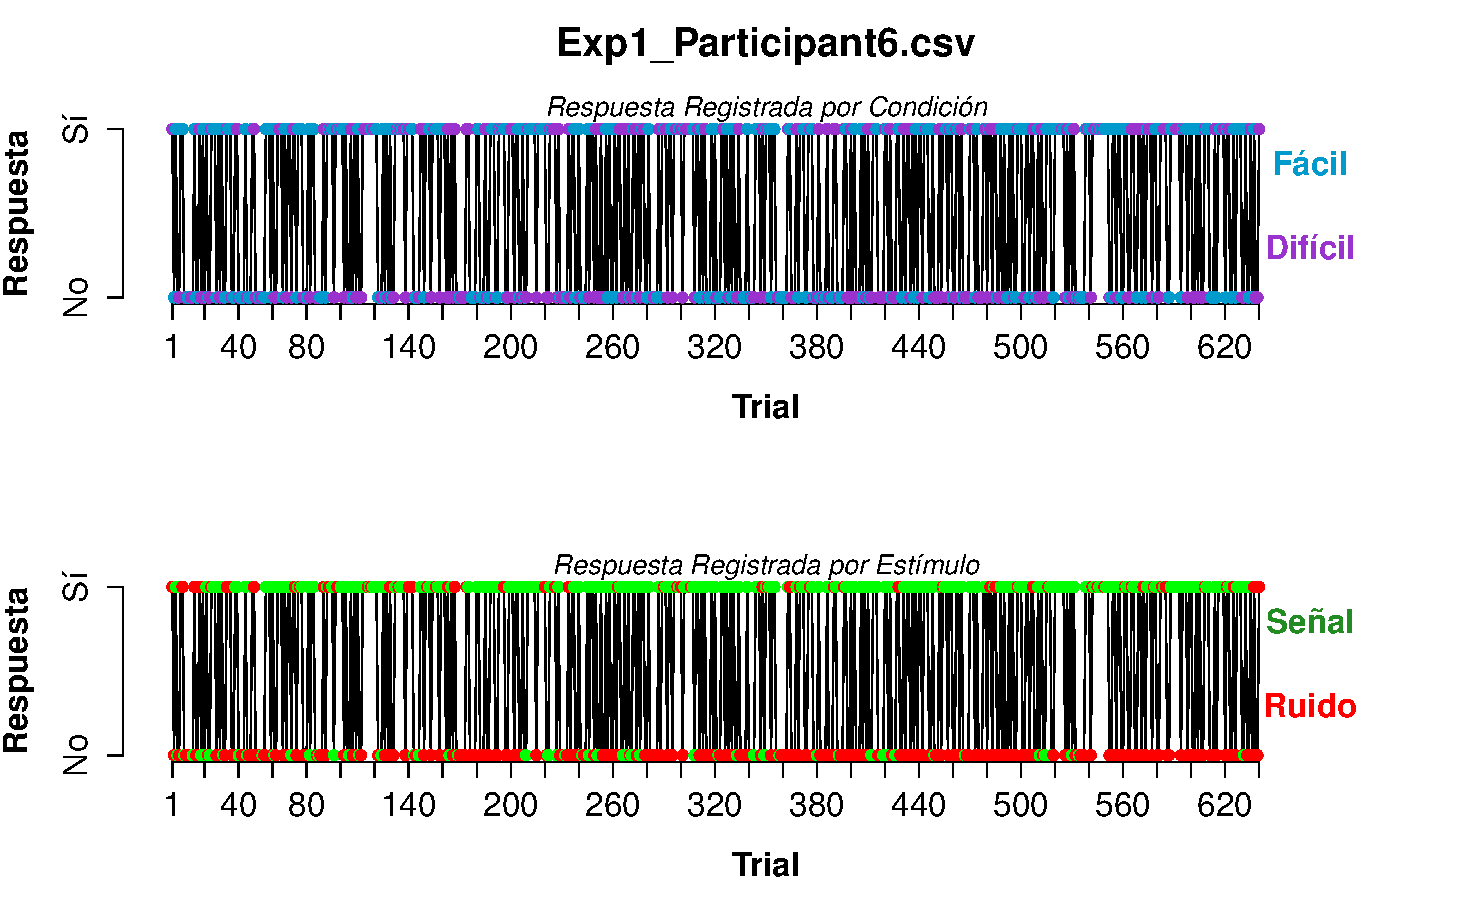
\includegraphics[width=0.30\textwidth]{Figures/BiasResp_Exp1_P6}
\includegraphics[width=0.30\textwidth]{Figures/BiasResp_Exp1_P7} \includegraphics[width=0.30\textwidth]{Figures/BiasResp_Exp1_P8} \includegraphics[width=0.30\textwidth]{Figures/BiasResp_Exp1_P9}
\includegraphics[width=0.30\textwidth]{Figures/BiasResp_Exp1_P10} \includegraphics[width=0.30\textwidth]{Figures/BiasResp_Exp1_P11} \includegraphics[width=0.30\textwidth]{Figures/BiasResp_Exp1_P12}
\includegraphics[width=0.30\textwidth]{Figures/BiasResp_Exp1_P13} \includegraphics[width=0.30\textwidth]{Figures/BiasResp_Exp1_P14} \includegraphics[width=0.30\textwidth]{Figures/BiasResp_Exp1_P15}
\includegraphics[width=0.30\textwidth]{Figures/BiasResp_Exp1_P16} \includegraphics[width=0.30\textwidth]{Figures/BiasResp_Exp1_P17} \includegraphics[width=0.30\textwidth]{Figures/BiasResp_Exp1_P18}
\includegraphics[width=0.30\textwidth]{Figures/BiasResp_Exp1_P19} \includegraphics[width=0.30\textwidth]{Figures/BiasResp_Exp1_P20} \includegraphics[width=0.30\textwidth]{Figures/BiasResp_Exp1_P21}
%\decoRule
\caption[Respuesta binaria registrada ensayo a ensayo en relación con el tipo de estímulo a evaluar; Experimento 1]{Respuesta registrada, ensayo a ensayo, durante la tarea de detección binaria por cada uno de los veintiun participantes del Experimento 1. Se muestran las elecciones de los participantes en tres distintas gráficas que señalan con diferentes colores las características de los estímulos a presentados en cada ensayo. Los gráficos superiores, distinguen entre el tipo de condición al que pertenecía el estímulo a evaluar por ensayo (i.e. En color púrpura, se señalan los ensayos con estímulos difíciles y en azul, con estímulos fáciles); el panel central distingue los ensayos que que contienen la señal y el ruido (en colores verde y rojo, respectivamente) y en la parte inferior se muestra un gráfico que señala el color del estímulo a veluar, con el color correspondiente.}
\label{fig:BiasResp_E1}
\end{figure}

\begin{figure}[th]
\centering
\includegraphics[width=0.30\textwidth]{Figures/BiasResp_Exp2_P1} \includegraphics[width=0.30\textwidth]{Figures/BiasResp_Exp2_P2} \includegraphics[width=0.30\textwidth]{Figures/BiasResp_Exp2_P3}
\includegraphics[width=0.30\textwidth]{Figures/BiasResp_Exp2_P4} \includegraphics[width=0.30\textwidth]{Figures/BiasResp_Exp2_P5} \includegraphics[width=0.30\textwidth]{Figures/BiasResp_Exp2_P6}
\includegraphics[width=0.30\textwidth]{Figures/BiasResp_Exp2_P7} \includegraphics[width=0.30\textwidth]{Figures/BiasResp_Exp2_P8} \includegraphics[width=0.30\textwidth]{Figures/BiasResp_Exp2_P9}
\includegraphics[width=0.30\textwidth]{Figures/BiasResp_Exp2_P10} \includegraphics[width=0.30\textwidth]{Figures/BiasResp_Exp2_P11} \includegraphics[width=0.30\textwidth]{Figures/BiasResp_Exp2_P12}
\includegraphics[width=0.30\textwidth]{Figures/BiasResp_Exp2_P13} \includegraphics[width=0.30\textwidth]{Figures/BiasResp_Exp2_P14} \includegraphics[width=0.30\textwidth]{Figures/BiasResp_Exp2_P15}
\includegraphics[width=0.30\textwidth]{Figures/BiasResp_Exp2_P16} \includegraphics[width=0.30\textwidth]{Figures/BiasResp_Exp2_P17} \includegraphics[width=0.30\textwidth]{Figures/BiasResp_Exp2_P18}
\includegraphics[width=0.30\textwidth]{Figures/BiasResp_Exp2_P19} \includegraphics[width=0.30\textwidth]{Figures/BiasResp_Exp2_P20}
%\decoRule
\caption[Respuesta binaria registrada ensayo a ensayo en relación con el tipo de estímulo a evaluar; Experimento 2]{Respuesta registrada, ensayo a ensayo, durante la tarea de detección binaria por cada uno de los participantes del Experimento 2. Se muestran las elecciones de los participantes en tres distintas gráficas que señalan con diferentes colores las características de los estímulos a presentados en cada ensayo. Los gráficos superiores, distinguen entre el tipo de condición al que pertenecía el estímulo a evaluar por ensayo (i.e. En color púrpura, se señalan los ensayos con estímulos difíciles y en azul, con estímulos fáciles); el panel central distingue los ensayos que que contienen la señal y el ruido (en colores verde y rojo, respectivamente) y en la parte inferior se muestra un gráfico que señala el color del estímulo a veluar, con el color correspondiente.}
\label{fig:BiasResp_E2}
\end{figure}

\begin{figure}[th]
\centering
\includegraphics[width=0.30\textwidth]{Figures/Rating_Exp1_P1} \includegraphics[width=0.30\textwidth]{Figures/Rating_Exp1_P2} \includegraphics[width=0.30\textwidth]{Figures/Rating_Exp1_P3}
\includegraphics[width=0.30\textwidth]{Figures/Rating_Exp1_P4} \includegraphics[width=0.30\textwidth]{Figures/Rating_Exp1_P5} \includegraphics[width=0.30\textwidth]{Figures/Rating_Exp1_P6}
\includegraphics[width=0.30\textwidth]{Figures/Rating_Exp1_P7} \includegraphics[width=0.30\textwidth]{Figures/Rating_Exp1_P8} \includegraphics[width=0.30\textwidth]{Figures/Rating_Exp1_P9}
\includegraphics[width=0.30\textwidth]{Figures/Rating_Exp1_P10} \includegraphics[width=0.30\textwidth]{Figures/Rating_Exp1_P11} \includegraphics[width=0.30\textwidth]{Figures/Rating_Exp1_P12}
\includegraphics[width=0.30\textwidth]{Figures/Rating_Exp1_P13} \includegraphics[width=0.30\textwidth]{Figures/Rating_Exp1_P14} \includegraphics[width=0.30\textwidth]{Figures/Rating_Exp1_P15}
\includegraphics[width=0.30\textwidth]{Figures/Rating_Exp1_P16} \includegraphics[width=0.30\textwidth]{Figures/Rating_Exp1_P17} \includegraphics[width=0.30\textwidth]{Figures/Rating_Exp1_P18}
\includegraphics[width=0.30\textwidth]{Figures/Rating_Exp1_P19} \includegraphics[width=0.30\textwidth]{Figures/Rating_Exp1_P20} \includegraphics[width=0.30\textwidth]{Figures/Rating_Exp1_P21}
%\decoRule
\caption[Puntajes de Confianza asignados ensayo a ensayo; Experimento 1]{Puntaje asignado, ensayo a ensayo, a las respuestas emitidas durante la tarea de detección binaria por cada uno de los participantes del Experimento 1. Las elecciones de cada participante se muestran en dos gráficos diferentes, donde se despliegan las respuestas dadas en la primer y segunda mitad del experimento (paneles superior e inferior, respectivamente). Durante el experimento, los participantes únicamente tuvieron que oprimir las teclas '1', '2' y '3', posteriormente el programa traducía estas respuestas en una escala mayor que distingue la certidumbre en la ausencia de la señal (i.e. '1' como 'muy seguro de que no') y la certidumbre de su presencia (i.e. '6' como 'muy seguro de que sí'). Dada esta transformación, es posible saber cuál fue la respuesta emitida por los participantes en la tarea binaria y qué tecla se oprimió para valorar su certidumbre.}
\label{fig:Rating_E1}
\end{figure}

\begin{figure}[th]
\centering
\includegraphics[width=0.30\textwidth]{Figures/Rating_Exp2_P1} \includegraphics[width=0.30\textwidth]{Figures/Rating_Exp2_P2} \includegraphics[width=0.30\textwidth]{Figures/Rating_Exp2_P3}
\includegraphics[width=0.30\textwidth]{Figures/Rating_Exp2_P4} \includegraphics[width=0.30\textwidth]{Figures/Rating_Exp2_P5} \includegraphics[width=0.30\textwidth]{Figures/Rating_Exp2_P6}
\includegraphics[width=0.30\textwidth]{Figures/Rating_Exp2_P7} \includegraphics[width=0.30\textwidth]{Figures/Rating_Exp2_P8} \includegraphics[width=0.30\textwidth]{Figures/Rating_Exp2_P9}
\includegraphics[width=0.30\textwidth]{Figures/Rating_Exp2_P10} \includegraphics[width=0.30\textwidth]{Figures/Rating_Exp2_P11} \includegraphics[width=0.30\textwidth]{Figures/Rating_Exp2_P12}
\includegraphics[width=0.30\textwidth]{Figures/Rating_Exp2_P13} \includegraphics[width=0.30\textwidth]{Figures/Rating_Exp2_P14} \includegraphics[width=0.30\textwidth]{Figures/Rating_Exp2_P15}
\includegraphics[width=0.30\textwidth]{Figures/Rating_Exp2_P16} \includegraphics[width=0.30\textwidth]{Figures/Rating_Exp2_P17} \includegraphics[width=0.30\textwidth]{Figures/Rating_Exp2_P18}
\includegraphics[width=0.30\textwidth]{Figures/Rating_Exp2_P19} \includegraphics[width=0.30\textwidth]{Figures/Rating_Exp2_P20} 
%\decoRule
\caption[Puntajes de Confianza asignados ensayo a ensayo; Experimento 2]{Puntaje asignado, ensayo a ensayo, a las respuestas emitidas durante la tarea de detección binaria por cada uno de los veinte participantes del Experimento 2. Las elecciones de cada participante se muestran en dos gráficos diferentes, donde se despliegan las respuestas dadas en la primer y segunda mitad del experimento (paneles superior e inferior, respectivamente). Durante el experimento, los participantes únicamente tuvieron que oprimir las teclas '1', '2' y '3', posteriormente el programa traducía estas respuestas en una escala mayor que distingue la certidumbre en la ausencia de la señal (i.e. '1' como 'muy seguro de que no') y la certidumbre de su presencia (i.e. '6' como 'muy seguro de que sí'). Dada esta transformación, es posible saber cuál fue la respuesta emitida por los participantes en la tarea binaria y qué tecla se oprimió para valorar su certidumbre.}
\label{fig:Rating_E2}
\end{figure}











\section{Control 2: ¿La duración del experimento tuvo un impacto en la ejecución de los participantes?}

Durante la tarea de detección binaria, los estímulos a comparar permanecían en pantalla 1.5 segundos en la pantalla antes de desaparecer, con independencia de si los participantes respondían, o no, antes de que se acabara dicho intervalo. Se controló la exposición a los estímulos para preveer que los participantes tuvieran ocasión de estudiar deteñidamente las figuras de Ebbinghaus mostradas y 'perder el efecto de la ilusión' cuanto más tiempo pasaran observándolas. Además, cuando los participantes asignaban un puntaje de confianza a esta primer respuesta binaria, se les mostraba una pantalla intermedia con la instrucción de oprimir la barra espaciadora cuando estuvieran listos para responder a un nuevo par de estímulos, en vez de simplemente arrojar el siguiente ensayo, buscando así que estuvieran atendiendo a los estímulos diseñados y permitiéndoles, además, la ocasión para tomar un breve respiro de la tarea. Estos dos controles incluídos en el procedimiento programado fueron hechos con el objetivo de preveer la habituación a la ilusión (i.e. una suerte de efecto de aprendizaje donde las ilusiones de Ebbinghaus pierden su intensidad) y la fatiga (i.e. que los participantes dejaran de prestar atención a los estímulos y emitieran sus respuestas a una tasa constante, conforme van apareciendo y desapareciendo los estímulos). Un segundo filtro en la revisión de nuestros datos, consta de la comparación visual del desempeño de los participantes a lo largo del tiempo: si la ejecución de los participantes se ve mermada considerablemente conforme avanzan los ensayos, podríamos identificar un claro efecto de fatiga, en tanto que si su ejecución mejora con el tiempo, podríamos sospechar de la influencia de un efecto de habituación o aprendizaje.


\begin{itemize}
\item Aciertos y errores a lo largo del tiempo

La manera más directa de observar cambios en el desempeño de los participantes a lo largo del tiempo es observar si las respuestas dadas por los participantes ensayo a ensayo fueron registradas como aciertos o errores, de acuerdo a su correspondencia con el tipo de estímulo presentado en pantalla y ver si conforme pasa el tiempo cambia la frecuencia con que los participantes cometen aciertos o errores. La Figura~\ref{fig:Success_E1_P14} presenta un ejemplo de este tipo de gráficas, tomando como ejemplo la ejecución del Participante 14 del Experimento 1. La obtención de aciertos y errores en el experimento se expresa de dos formas, mediante la acumulación de aciertos y errores a lo largo del tiempo (la gráfica de frecuencias acumuladas en la parte superior) y señalando, ensayo a ensayo, si el participante ha cometido un acierto o un error (los páneles medio e inferior, donde se muestra por separado la ejecución del participante durante la primera y segunda mitad del experimento).


\begin{figure}[th]
\centering
\includegraphics[width=0.60\textwidth]{Figures/Success_Exp1_P14}
%\decoRule
\caption[Aciertos y errores a lo largo del tiempo: Ejemplo]{Aciertos y errores cometidos por el Participante 14 del Experimento 1 a lo largo del tiempo. En el panel superior se muestra la frecuencia acumulada de aciertos y errores cometidos en el tiempo, en tanto que los paneles inferiores muestran el registro de las respuestas del participante como Aciertos o Errores en cada ensayo, de acuerdo a su correspondencia con el estímulo evaluado. El panel intermedio muestra los aciertos y errores registrados durante la primer mitad de la tarea, y el panel inferior muestra el resto.}
\label{fig:Success_E1_P14}
\end{figure}

Las Figuras~\ref{fig:Success_E1} y \ref{fig:Success_E2} muestran los aciertos y errores acumulados y cometidos a lo largo del tiempo para el resto de los participantes en los experimentos 1 y 2, respectivamente.


\item Resultados obtenidos a lo largo del tiempo

Una manera más fina de visualizar los aciertos y errores cometidos a lo largo de la tarea, es separar y señalar los posibles tipos de aciertos (Hits y Rechazos) y errores (Falsas alarmas y Omisiones), que se hayan cometido en cada ensayo. Por ejemplo, la Figura~\ref{fig:Outcome_E1_P14} muestra los resultados obtenidos por el Participante 14 del Experimento 1 al emitir cada una de sus respuestas durante la tarea binaria. El panel superior muestra la frecuencia acumulada de cada uno de los posibles resultados (Hits, Falsas Alarmas, Rechazos y Omisiones) y el inferior, el resultado obtenido en cada uno de los ensayos. El resto de los participantes en los experimentos 1 y 2 aparecen en las Figuras~\ref{fig:Outcome_E1} y \ref{fig:Outcome_E2}, respectivamente.

\begin{figure}[th]
\centering
\includegraphics[width=0.60\textwidth]{Figures/Outcome_Exp1_P6}
%\decoRule
\caption[Resultado obtenido a lo largo del tiempo: Ejemplo]{Resultado obtenido por el Participante 6 del Experimento 1, dada cada una de sus respuestas a lo largo del Experimento. El panel superior muestra la frecuencia acumulada de Hits, Falsas Alarmas, Rechazos y Omisiones obtenidos durante el experimento; el panel inferior muestra el tipo de resultado registrado en cada uno de los 640 ensayos.}
\label{fig:Outcome_E1_P14}
\end{figure}



\end{itemize}

\begin{figure}[th]
\centering
\includegraphics[width=0.30\textwidth]{Figures/Success_Exp1_P1} \includegraphics[width=0.30\textwidth]{Figures/Success_Exp1_P2} \includegraphics[width=0.30\textwidth]{Figures/Success_Exp1_P3}
\includegraphics[width=0.30\textwidth]{Figures/Success_Exp1_P4} \includegraphics[width=0.30\textwidth]{Figures/Success_Exp1_P5} \includegraphics[width=0.30\textwidth]{Figures/Success_Exp1_P6}
\includegraphics[width=0.30\textwidth]{Figures/Success_Exp1_P7} \includegraphics[width=0.30\textwidth]{Figures/Success_Exp1_P8} \includegraphics[width=0.30\textwidth]{Figures/Success_Exp1_P9}
\includegraphics[width=0.30\textwidth]{Figures/Success_Exp1_P10} \includegraphics[width=0.30\textwidth]{Figures/Success_Exp1_P11} \includegraphics[width=0.30\textwidth]{Figures/Success_Exp1_P12}
\includegraphics[width=0.30\textwidth]{Figures/Success_Exp1_P13} \includegraphics[width=0.30\textwidth]{Figures/Success_Exp1_P14} \includegraphics[width=0.30\textwidth]{Figures/Success_Exp1_P15}
\includegraphics[width=0.30\textwidth]{Figures/Success_Exp1_P16} \includegraphics[width=0.30\textwidth]{Figures/Success_Exp1_P17} \includegraphics[width=0.30\textwidth]{Figures/Success_Exp1_P18}
\includegraphics[width=0.30\textwidth]{Figures/Success_Exp1_P19} \includegraphics[width=0.30\textwidth]{Figures/Success_Exp1_P20} \includegraphics[width=0.30\textwidth]{Figures/Success_Exp1_P21} 
%\decoRule
\caption[Aciertos y Errores a lo largo del tiempo; Experimento 1]{Aciertos y errores cometidos por los participantes del Experimento 1. Por cada participante se muestran la frecuencia acumulada de aciertos y errores (Panel superior) y los aciertos y errores cometidos durante la primera y segunda mitad del experimento (paneles intermedio e inferior, respectivamente).}
\label{fig:Success_E1}
\end{figure}

\begin{figure}[th]
\centering
\includegraphics[width=0.30\textwidth]{Figures/Success_Exp2_P1} \includegraphics[width=0.30\textwidth]{Figures/Success_Exp2_P2} \includegraphics[width=0.30\textwidth]{Figures/Success_Exp2_P3}
\includegraphics[width=0.30\textwidth]{Figures/Success_Exp2_P4} \includegraphics[width=0.30\textwidth]{Figures/Success_Exp2_P5} \includegraphics[width=0.30\textwidth]{Figures/Success_Exp2_P6}
\includegraphics[width=0.30\textwidth]{Figures/Success_Exp2_P7} \includegraphics[width=0.30\textwidth]{Figures/Success_Exp2_P8} \includegraphics[width=0.30\textwidth]{Figures/Success_Exp2_P9}
\includegraphics[width=0.30\textwidth]{Figures/Success_Exp2_P10} \includegraphics[width=0.30\textwidth]{Figures/Success_Exp2_P11} \includegraphics[width=0.30\textwidth]{Figures/Success_Exp2_P12}
\includegraphics[width=0.30\textwidth]{Figures/Success_Exp2_P13} \includegraphics[width=0.30\textwidth]{Figures/Success_Exp2_P14} \includegraphics[width=0.30\textwidth]{Figures/Success_Exp2_P15}
\includegraphics[width=0.30\textwidth]{Figures/Success_Exp2_P16} \includegraphics[width=0.30\textwidth]{Figures/Success_Exp2_P17} \includegraphics[width=0.30\textwidth]{Figures/Success_Exp2_P18}
\includegraphics[width=0.30\textwidth]{Figures/Success_Exp2_P19} \includegraphics[width=0.30\textwidth]{Figures/Success_Exp2_P20} 
%\decoRule
\caption[Aciertos y Errores a lo largo del tiempo; Experimento 2]{Aciertos y errores cometidos en el Experimento 2 por cada uno de los participantes. Se muestran las frecuencias acumuladas de aciertos y errores a lo largo del tiempo (panel superior) y el registro de un acierto o error en cada uno de los ensayos para la primera y segunda mitad del procedimiento (paneles intermedio e inferior, respectivamente).}
\label{fig:Success_E2}
\end{figure}

\begin{figure}[th]
\centering
\includegraphics[width=0.30\textwidth]{Figures/Outcome_Exp1_P1} \includegraphics[width=0.30\textwidth]{Figures/Outcome_Exp1_P2} \includegraphics[width=0.30\textwidth]{Figures/Outcome_Exp1_P3}
\includegraphics[width=0.30\textwidth]{Figures/Outcome_Exp1_P4} \includegraphics[width=0.30\textwidth]{Figures/Outcome_Exp1_P5} \includegraphics[width=0.30\textwidth]{Figures/Outcome_Exp1_P6}
\includegraphics[width=0.30\textwidth]{Figures/Outcome_Exp1_P7} \includegraphics[width=0.30\textwidth]{Figures/Outcome_Exp1_P8} \includegraphics[width=0.30\textwidth]{Figures/Outcome_Exp1_P9}
\includegraphics[width=0.30\textwidth]{Figures/Outcome_Exp1_P10} \includegraphics[width=0.30\textwidth]{Figures/Outcome_Exp1_P11} \includegraphics[width=0.30\textwidth]{Figures/Outcome_Exp1_P12}
\includegraphics[width=0.30\textwidth]{Figures/Outcome_Exp1_P13} \includegraphics[width=0.30\textwidth]{Figures/Outcome_Exp1_P14} \includegraphics[width=0.30\textwidth]{Figures/Outcome_Exp1_P15}
\includegraphics[width=0.30\textwidth]{Figures/Outcome_Exp1_P16} \includegraphics[width=0.30\textwidth]{Figures/Outcome_Exp1_P17} \includegraphics[width=0.30\textwidth]{Figures/Outcome_Exp1_P18}
\includegraphics[width=0.30\textwidth]{Figures/Outcome_Exp1_P19} \includegraphics[width=0.30\textwidth]{Figures/Outcome_Exp1_P20} \includegraphics[width=0.30\textwidth]{Figures/Outcome_Exp1_P21} 
%\decoRule
\caption[Resultados obtenidos por ensayo; Experimento 1]{Resultado obtenido en cada ensayo por cada participante del Experimento 1. En el panel superior, se muestran las frecuencias acumuladas de los Hits, Falsas Alarmas, Rechazos y Omisiones cometidos durante el experimento y en el panel inferior, se señala ensayo a ensayo si el participante emitió una respuesa acertada o errónea.}
\label{fig:Outcome_E1}
\end{figure}

\begin{figure}[th]
\centering
\includegraphics[width=0.30\textwidth]{Figures/Outcome_Exp2_P1} \includegraphics[width=0.30\textwidth]{Figures/Outcome_Exp2_P2} \includegraphics[width=0.30\textwidth]{Figures/Outcome_Exp2_P3}
\includegraphics[width=0.30\textwidth]{Figures/Outcome_Exp2_P4} \includegraphics[width=0.30\textwidth]{Figures/Outcome_Exp2_P5} \includegraphics[width=0.30\textwidth]{Figures/Outcome_Exp2_P6}
\includegraphics[width=0.30\textwidth]{Figures/Outcome_Exp2_P7} \includegraphics[width=0.30\textwidth]{Figures/Outcome_Exp2_P8} \includegraphics[width=0.30\textwidth]{Figures/Outcome_Exp2_P9}
\includegraphics[width=0.30\textwidth]{Figures/Outcome_Exp2_P10} \includegraphics[width=0.30\textwidth]{Figures/Outcome_Exp2_P11} \includegraphics[width=0.30\textwidth]{Figures/Outcome_Exp2_P12}
\includegraphics[width=0.30\textwidth]{Figures/Outcome_Exp2_P13} \includegraphics[width=0.30\textwidth]{Figures/Outcome_Exp2_P14} \includegraphics[width=0.30\textwidth]{Figures/Outcome_Exp2_P15}
\includegraphics[width=0.30\textwidth]{Figures/Outcome_Exp2_P16} \includegraphics[width=0.30\textwidth]{Figures/Outcome_Exp2_P17} \includegraphics[width=0.30\textwidth]{Figures/Outcome_Exp2_P18}
\includegraphics[width=0.30\textwidth]{Figures/Outcome_Exp2_P19} \includegraphics[width=0.30\textwidth]{Figures/Outcome_Exp2_P20} 
%\decoRule
\caption[Resultados obtenidos por ensayo; Experimento 2]{Resultados obtenidos por cada uno de los participantes del Experimento 2. En el panel superior se muestran las frecuencias acumuladas de Hits, Falsas alarmas, Rehazos y Omisiones, y en el panel inferior se muestran los aciertos o errores cometidos en cada uno de los 640 ensayos del experimento.}
\label{fig:Outcome_E2}
\end{figure}












\section{Control 3: ¿Las variables mezcladas para construir los estímulos están afectando el desempeño de los participantes?}



\begin{itemize}
\item El efecto del Color
\item El Efecto del Numero de Círculos Externos
\end{itemize}

\begin{figure}[th]
\centering
\includegraphics[width=0.30\textwidth]{Figures/Color_Exp1_P1} \includegraphics[width=0.30\textwidth]{Figures/Color_Exp1_P2} \includegraphics[width=0.30\textwidth]{Figures/Color_Exp1_P3}
\includegraphics[width=0.30\textwidth]{Figures/Color_Exp1_P4} \includegraphics[width=0.30\textwidth]{Figures/Color_Exp1_P5} \includegraphics[width=0.30\textwidth]{Figures/Color_Exp1_P6}
\includegraphics[width=0.30\textwidth]{Figures/Color_Exp1_P7} \includegraphics[width=0.30\textwidth]{Figures/Color_Exp1_P8} \includegraphics[width=0.30\textwidth]{Figures/Color_Exp1_P9}
\includegraphics[width=0.30\textwidth]{Figures/Color_Exp1_P10} \includegraphics[width=0.30\textwidth]{Figures/Color_Exp1_P11} \includegraphics[width=0.30\textwidth]{Figures/Color_Exp1_P12}
\includegraphics[width=0.30\textwidth]{Figures/Color_Exp1_P13} \includegraphics[width=0.30\textwidth]{Figures/Color_Exp1_P14} \includegraphics[width=0.30\textwidth]{Figures/Color_Exp1_P15}
\includegraphics[width=0.30\textwidth]{Figures/Color_Exp1_P16} \includegraphics[width=0.30\textwidth]{Figures/Color_Exp1_P17} \includegraphics[width=0.30\textwidth]{Figures/Color_Exp1_P18}
\includegraphics[width=0.30\textwidth]{Figures/Color_Exp1_P19} \includegraphics[width=0.30\textwidth]{Figures/Color_Exp1_P20} \includegraphics[width=0.30\textwidth]{Figures/Color_Exp1_P21} 
%\decoRule
\caption[Color_Exp1]{}
\label{fig:Color_E1}
\end{figure}

\begin{figure}[th]
\centering
\includegraphics[width=0.30\textwidth]{Figures/Color_Exp2_P1} \includegraphics[width=0.30\textwidth]{Figures/Color_Exp2_P2} \includegraphics[width=0.30\textwidth]{Figures/Color_Exp2_P3}
\includegraphics[width=0.30\textwidth]{Figures/Color_Exp2_P4} \includegraphics[width=0.30\textwidth]{Figures/Color_Exp2_P5} \includegraphics[width=0.30\textwidth]{Figures/Color_Exp2_P6}
\includegraphics[width=0.30\textwidth]{Figures/Color_Exp2_P7} \includegraphics[width=0.30\textwidth]{Figures/Color_Exp2_P8} \includegraphics[width=0.30\textwidth]{Figures/Color_Exp2_P9}
\includegraphics[width=0.30\textwidth]{Figures/Color_Exp2_P10} \includegraphics[width=0.30\textwidth]{Figures/Color_Exp2_P11} \includegraphics[width=0.30\textwidth]{Figures/Color_Exp2_P12}
\includegraphics[width=0.30\textwidth]{Figures/Color_Exp2_P13} \includegraphics[width=0.30\textwidth]{Figures/Color_Exp2_P14} \includegraphics[width=0.30\textwidth]{Figures/Color_Exp2_P15}
\includegraphics[width=0.30\textwidth]{Figures/Color_Exp2_P16} \includegraphics[width=0.30\textwidth]{Figures/Color_Exp2_P17} \includegraphics[width=0.30\textwidth]{Figures/Color_Exp2_P18}
\includegraphics[width=0.30\textwidth]{Figures/Color_Exp2_P19} \includegraphics[width=0.30\textwidth]{Figures/Color_Exp2_P20} 
%\decoRule
\caption[Color_Exp2]{}
\label{fig:Color_E2}
\end{figure}



\begin{figure}[th]
\centering
\includegraphics[width=0.30\textwidth]{Figures/Numero_Exp2_P1} \includegraphics[width=0.30\textwidth]{Figures/Numero_Exp2_P2} \includegraphics[width=0.30\textwidth]{Figures/Numero_Exp2_P3}
\includegraphics[width=0.30\textwidth]{Figures/Numero_Exp2_P4} \includegraphics[width=0.30\textwidth]{Figures/Numero_Exp2_P5} \includegraphics[width=0.30\textwidth]{Figures/Numero_Exp2_P6}
\includegraphics[width=0.30\textwidth]{Figures/Numero_Exp2_P7} \includegraphics[width=0.30\textwidth]{Figures/Numero_Exp2_P8} \includegraphics[width=0.30\textwidth]{Figures/Numero_Exp2_P9}
\includegraphics[width=0.30\textwidth]{Figures/Numero_Exp2_P10} \includegraphics[width=0.30\textwidth]{Figures/Numero_Exp2_P11} \includegraphics[width=0.30\textwidth]{Figures/Numero_Exp2_P12}
\includegraphics[width=0.30\textwidth]{Figures/Numero_Exp2_P13} \includegraphics[width=0.30\textwidth]{Figures/Numero_Exp2_P14} \includegraphics[width=0.30\textwidth]{Figures/Numero_Exp2_P15}
\includegraphics[width=0.30\textwidth]{Figures/Numero_Exp2_P16} \includegraphics[width=0.30\textwidth]{Figures/Numero_Exp2_P17} \includegraphics[width=0.30\textwidth]{Figures/Numero_Exp2_P18}
\includegraphics[width=0.30\textwidth]{Figures/Numero_Exp2_P19} \includegraphics[width=0.30\textwidth]{Figures/Numero_Exp2_P20} 
%\decoRule
\caption[Numero_Exp2]{Efecto del Numero de Circulos Externos (Experimento 2).}
\label{fig:Numero_E2}
\end{figure}











\section{Evidencia del Efecto Espejo}

El último monitoreo de los datos antes de comenzar con los análisis estadísticos, estuvo enfocado en buscar los patrones de respuesta identificados como parte del Efecto Espejo. 

\begin{itemize}
\item Patrón de Hits y Falsas Alarmas
\item Patrón de Puntaje de Confianza
\end{itemize}

\begin{figure}[th]
\centering
\includegraphics[width=0.30\textwidth]{Figures/MirrorRate_Exp1_P1} \includegraphics[width=0.30\textwidth]{Figures/MirrorRate_Exp1_P2} \includegraphics[width=0.30\textwidth]{Figures/MirrorRate_Exp1_P3}
\includegraphics[width=0.30\textwidth]{Figures/MirrorRate_Exp1_P4} \includegraphics[width=0.30\textwidth]{Figures/MirrorRate_Exp1_P5} \includegraphics[width=0.30\textwidth]{Figures/MirrorRate_Exp1_P6}
\includegraphics[width=0.30\textwidth]{Figures/MirrorRate_Exp1_P7} \includegraphics[width=0.30\textwidth]{Figures/MirrorRate_Exp1_P8} \includegraphics[width=0.30\textwidth]{Figures/MirrorRate_Exp1_P9}
\includegraphics[width=0.30\textwidth]{Figures/MirrorRate_Exp1_P10} \includegraphics[width=0.30\textwidth]{Figures/MirrorRate_Exp1_P11} \includegraphics[width=0.30\textwidth]{Figures/MirrorRate_Exp1_P12}
\includegraphics[width=0.30\textwidth]{Figures/MirrorRate_Exp1_P13} \includegraphics[width=0.30\textwidth]{Figures/MirrorRate_Exp1_P14} \includegraphics[width=0.30\textwidth]{Figures/MirrorRate_Exp1_P15}
\includegraphics[width=0.30\textwidth]{Figures/MirrorRate_Exp1_P16} \includegraphics[width=0.30\textwidth]{Figures/MirrorRate_Exp1_P17} \includegraphics[width=0.30\textwidth]{Figures/MirrorRate_Exp1_P18}
\includegraphics[width=0.30\textwidth]{Figures/MirrorRate_Exp1_P19} \includegraphics[width=0.30\textwidth]{Figures/MirrorRate_Exp1_P20} \includegraphics[width=0.30\textwidth]{Figures/MirrorRate_Exp1_P21} 
%\decoRule
\caption[Rate_Exp1]{Comparando los Hits y Falsas Alarmas entre condiciones, de cada uno de los participantes del Experimento 1.}
\label{fig:Rate_E1}
\end{figure}

\begin{figure}[th]
\centering
\includegraphics[width=0.30\textwidth]{Figures/MirrorRate_Exp2_P1} \includegraphics[width=0.30\textwidth]{Figures/MirrorRate_Exp2_P2} \includegraphics[width=0.30\textwidth]{Figures/MirrorRate_Exp2_P3}
\includegraphics[width=0.30\textwidth]{Figures/MirrorRate_Exp2_P4} \includegraphics[width=0.30\textwidth]{Figures/MirrorRate_Exp2_P5} \includegraphics[width=0.30\textwidth]{Figures/MirrorRate_Exp2_P6}
\includegraphics[width=0.30\textwidth]{Figures/MirrorRate_Exp2_P7} \includegraphics[width=0.30\textwidth]{Figures/MirrorRate_Exp2_P8} \includegraphics[width=0.30\textwidth]{Figures/MirrorRate_Exp2_P9}
\includegraphics[width=0.30\textwidth]{Figures/MirrorRate_Exp2_P10} \includegraphics[width=0.30\textwidth]{Figures/MirrorRate_Exp2_P11} \includegraphics[width=0.30\textwidth]{Figures/MirrorRate_Exp2_P12}
\includegraphics[width=0.30\textwidth]{Figures/MirrorRate_Exp2_P13} \includegraphics[width=0.30\textwidth]{Figures/MirrorRate_Exp2_P14} \includegraphics[width=0.30\textwidth]{Figures/MirrorRate_Exp2_P15}
\includegraphics[width=0.30\textwidth]{Figures/MirrorRate_Exp2_P16} \includegraphics[width=0.30\textwidth]{Figures/MirrorRate_Exp2_P17} \includegraphics[width=0.30\textwidth]{Figures/MirrorRate_Exp2_P18}
\includegraphics[width=0.30\textwidth]{Figures/MirrorRate_Exp2_P19} \includegraphics[width=0.30\textwidth]{Figures/MirrorRate_Exp2_P20} 
%\decoRule
\caption[Rate_Exp2]{Comparación entre condiciones de los Hits y Falsas Alarmas}
\label{fig:Rate_E2}
\end{figure}

\begin{figure}[th]
\centering
\includegraphics[width=0.30\textwidth]{Figures/MirrorRating_Exp1_P1} \includegraphics[width=0.30\textwidth]{Figures/MirrorRating_Exp1_P2} \includegraphics[width=0.30\textwidth]{Figures/MirrorRating_Exp1_P3}
\includegraphics[width=0.30\textwidth]{Figures/MirrorRating_Exp1_P4} \includegraphics[width=0.30\textwidth]{Figures/MirrorRating_Exp1_P5} \includegraphics[width=0.30\textwidth]{Figures/MirrorRating_Exp1_P6}
\includegraphics[width=0.30\textwidth]{Figures/MirrorRating_Exp1_P7} \includegraphics[width=0.30\textwidth]{Figures/MirrorRating_Exp1_P8} \includegraphics[width=0.30\textwidth]{Figures/MirrorRating_Exp1_P9}
\includegraphics[width=0.30\textwidth]{Figures/MirrorRating_Exp1_P10} \includegraphics[width=0.30\textwidth]{Figures/MirrorRating_Exp1_P11} \includegraphics[width=0.30\textwidth]{Figures/MirrorRating_Exp1_P12}
\includegraphics[width=0.30\textwidth]{Figures/MirrorRating_Exp1_P13} \includegraphics[width=0.30\textwidth]{Figures/MirrorRating_Exp1_P14} \includegraphics[width=0.30\textwidth]{Figures/MirrorRating_Exp1_P15}
\includegraphics[width=0.30\textwidth]{Figures/MirrorRating_Exp1_P16} \includegraphics[width=0.30\textwidth]{Figures/MirrorRating_Exp1_P17} \includegraphics[width=0.30\textwidth]{Figures/MirrorRating_Exp1_P18}
\includegraphics[width=0.30\textwidth]{Figures/MirrorRating_Exp1_P19} \includegraphics[width=0.30\textwidth]{Figures/MirrorRating_Exp1_P20} \includegraphics[width=0.30\textwidth]{Figures/MirrorRating_Exp1_P21} 
%\decoRule
\caption[MErating_Ex1]{Evaluando el patrón de puntajes de confianza asignados (Experimento 1)}
\label{fig:MERating_E1}
\end{figure}

\begin{figure}[th]
\centering
\includegraphics[width=0.30\textwidth]{Figures/MirrorRating_Exp2_P1} \includegraphics[width=0.30\textwidth]{Figures/MirrorRating_Exp2_P2} \includegraphics[width=0.30\textwidth]{Figures/MirrorRating_Exp2_P3}
\includegraphics[width=0.30\textwidth]{Figures/MirrorRating_Exp2_P4} \includegraphics[width=0.30\textwidth]{Figures/MirrorRating_Exp2_P5} \includegraphics[width=0.30\textwidth]{Figures/MirrorRating_Exp2_P6}
\includegraphics[width=0.30\textwidth]{Figures/MirrorRating_Exp2_P7} \includegraphics[width=0.30\textwidth]{Figures/MirrorRating_Exp2_P8} \includegraphics[width=0.30\textwidth]{Figures/MirrorRating_Exp2_P9}
\includegraphics[width=0.30\textwidth]{Figures/MirrorRating_Exp2_P10} \includegraphics[width=0.30\textwidth]{Figures/MirrorRating_Exp2_P11} \includegraphics[width=0.30\textwidth]{Figures/MirrorRating_Exp2_P12}
\includegraphics[width=0.30\textwidth]{Figures/MirrorRating_Exp2_P13} \includegraphics[width=0.30\textwidth]{Figures/MirrorRating_Exp2_P14} \includegraphics[width=0.30\textwidth]{Figures/MirrorRating_Exp2_P15}
\includegraphics[width=0.30\textwidth]{Figures/MirrorRating_Exp2_P16} \includegraphics[width=0.30\textwidth]{Figures/MirrorRating_Exp2_P17} \includegraphics[width=0.30\textwidth]{Figures/MirrorRating_Exp2_P18}
\includegraphics[width=0.30\textwidth]{Figures/MirrorRating_Exp2_P19} \includegraphics[width=0.30\textwidth]{Figures/MirrorRating_Exp2_P20} 
%\decoRule
\caption[MERating_Exp2]{Evaluando el patrón de puntajes de confianza identificados como Efecto Espejo (Experimento 2)}
\label{fig:MERating_E2}
\end{figure}
